\section{Experiments and Results}

\subsection{Performance Evaluation}
The tests were run on 100, 500 and 1000 partitions, with several support values - the values were adjusted . The following sections will present comparisons of time performance and generated tree-sizes between different scenarios. 

[TODO: Add table of experiments summary - e.g. different datasets with the sizes]

\subsubsection{Standalone}
\label{sec:resultsstand}
We first evaluate each algorithm with different partition sizes to better understand its behaviour.
\paragraph{PFP}
~\autoref{fig:kosarak_pfp_001} presents PFP performance on ~\autoref{data:kosarak} with different partitions sizes. Best performance achieved for 500 partitions. For ~\autoref{data:10Msynt} ~\autoref{fig:T15I5D10000N100_pfp_0001}, best performance is achieved for 1000 partitions. And ~\autoref{fig:T15I5D1000N10_pfp_00001} for ~\autoref{data:1Msynt} with support of 0.00001 (more than 10 items are frequent). 100 and 500 have the better performance.


\begin{figure}[H]
  \centering
  \begin{subfigure}{\textwidth}
  \centering
  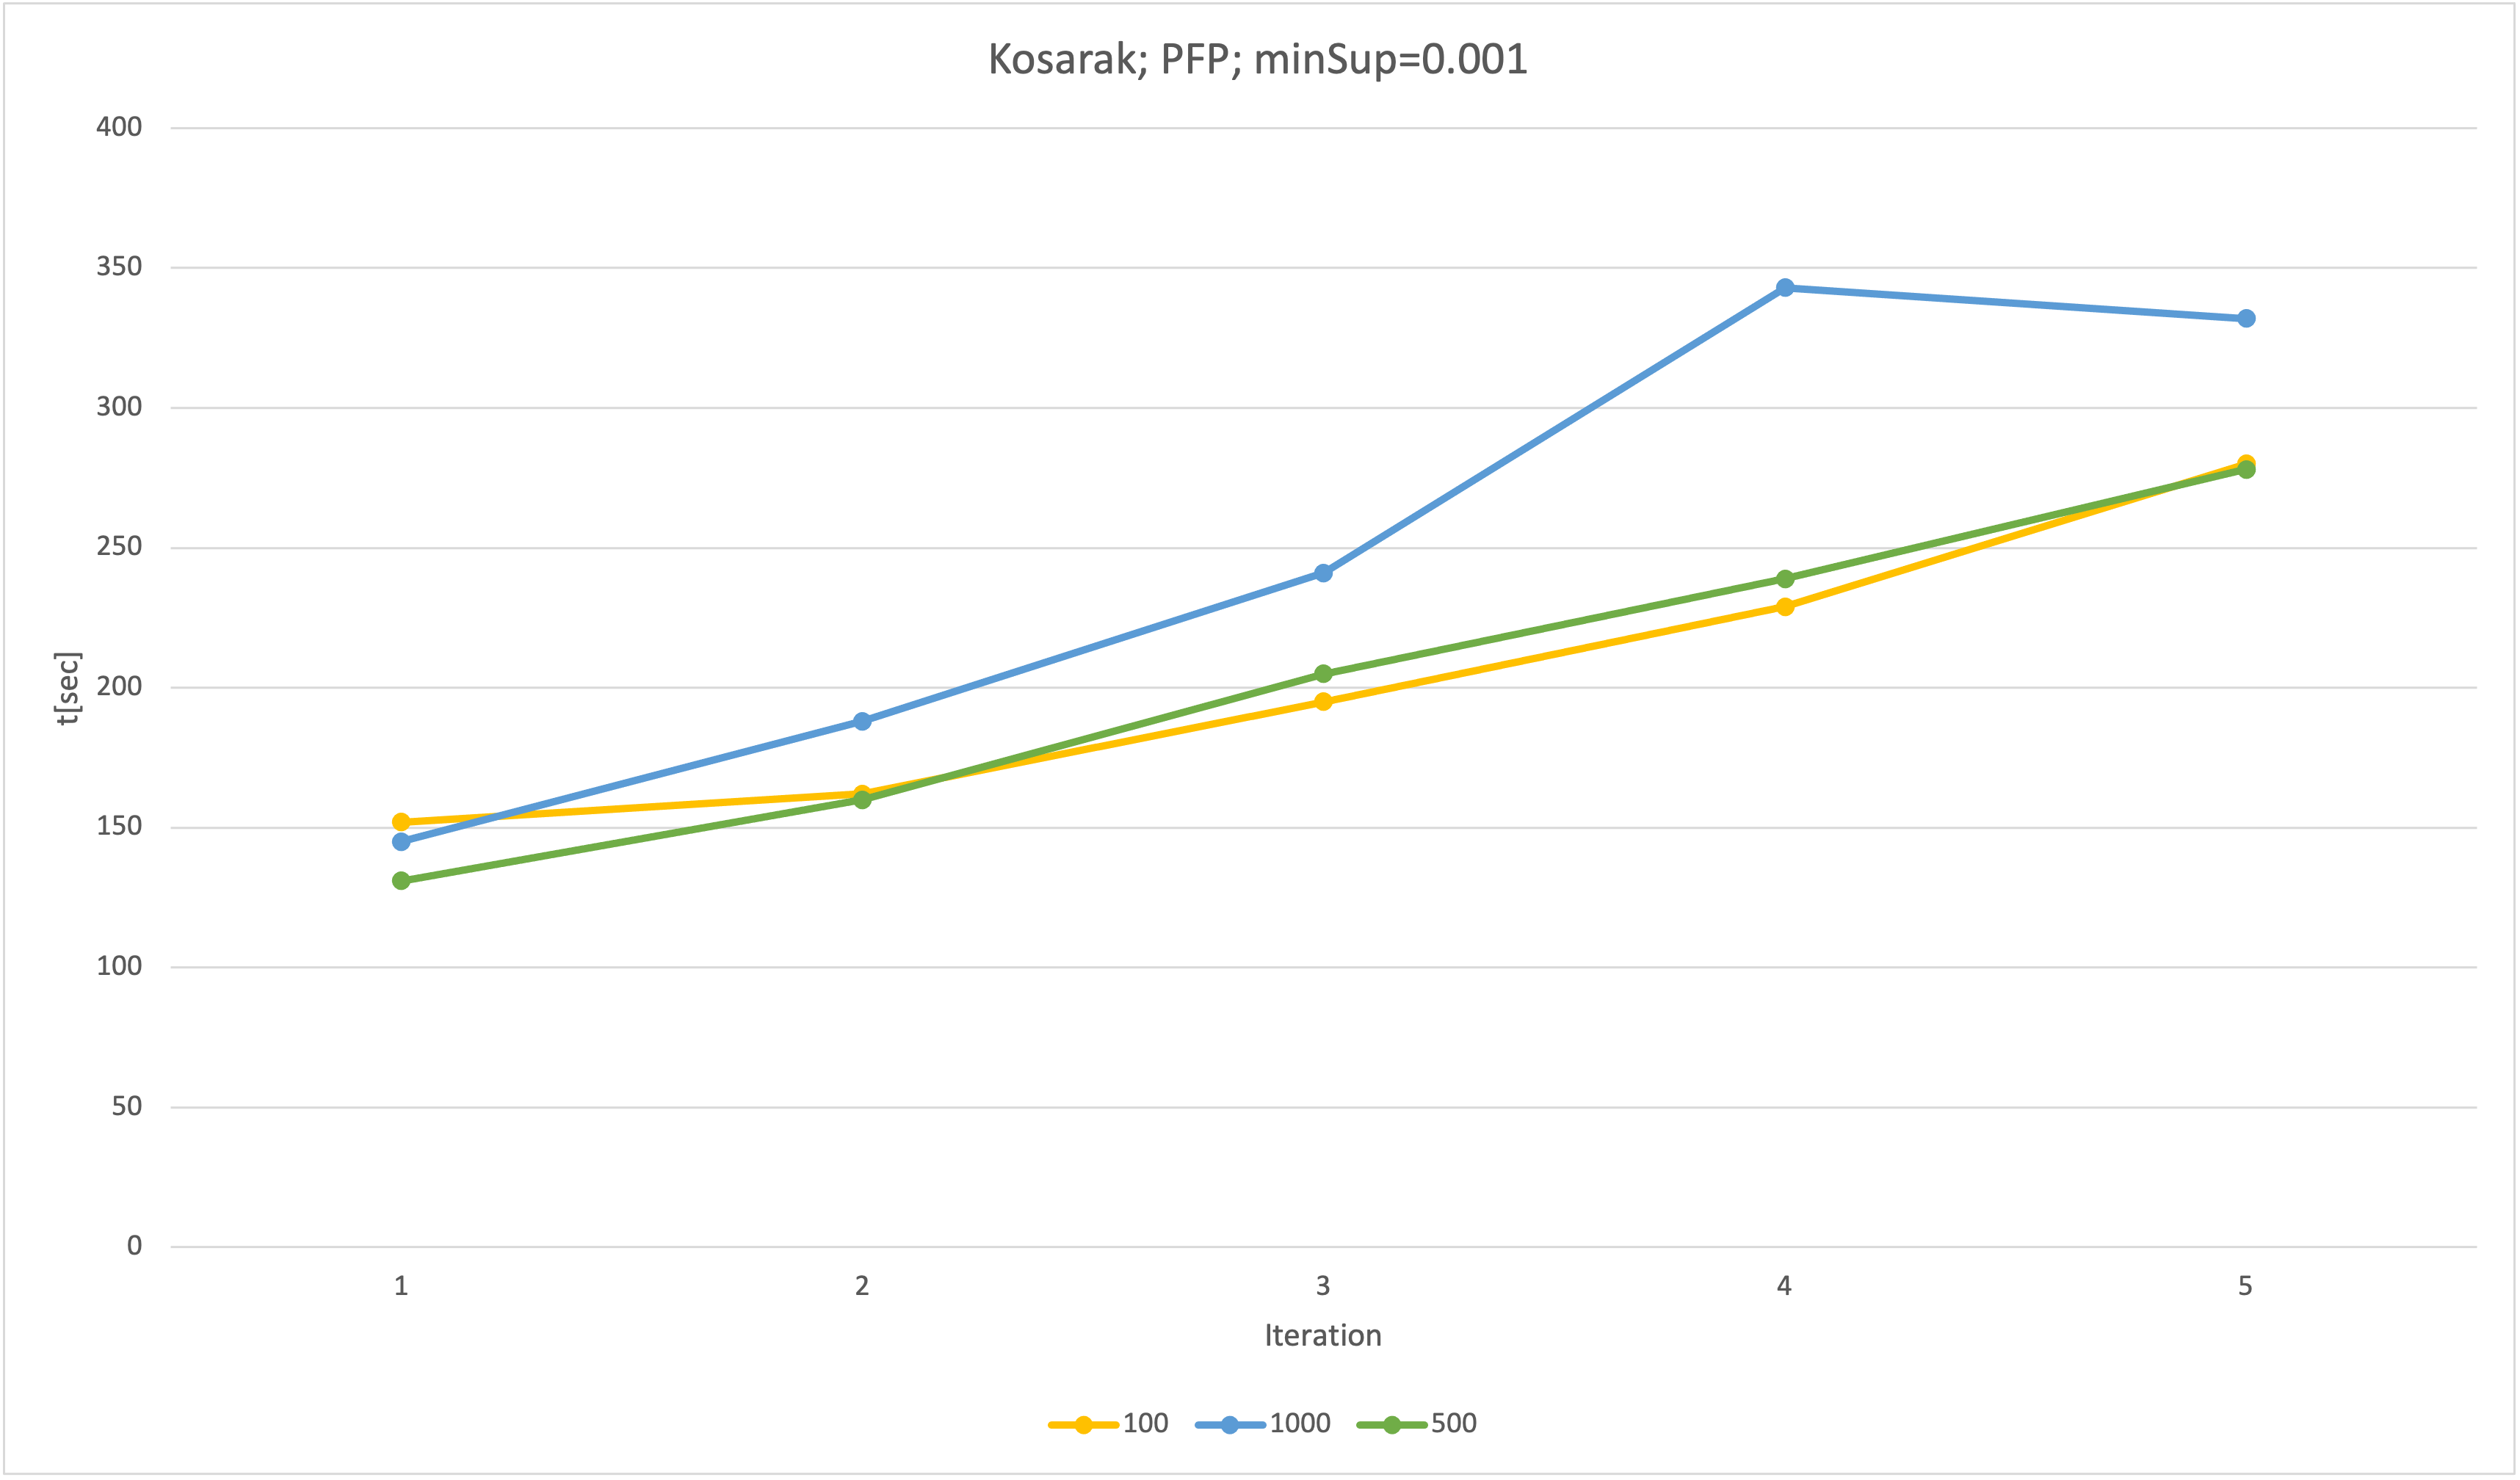
\includegraphics[width=\linewidth]{figures/4iterations/kosarak_pfp_001}
  \caption{kosarak, minSup = 0.001}
  \label{fig:kosarak_pfp_001}
  \end{subfigure}
  \begin{subfigure}{\textwidth}
  \centering
  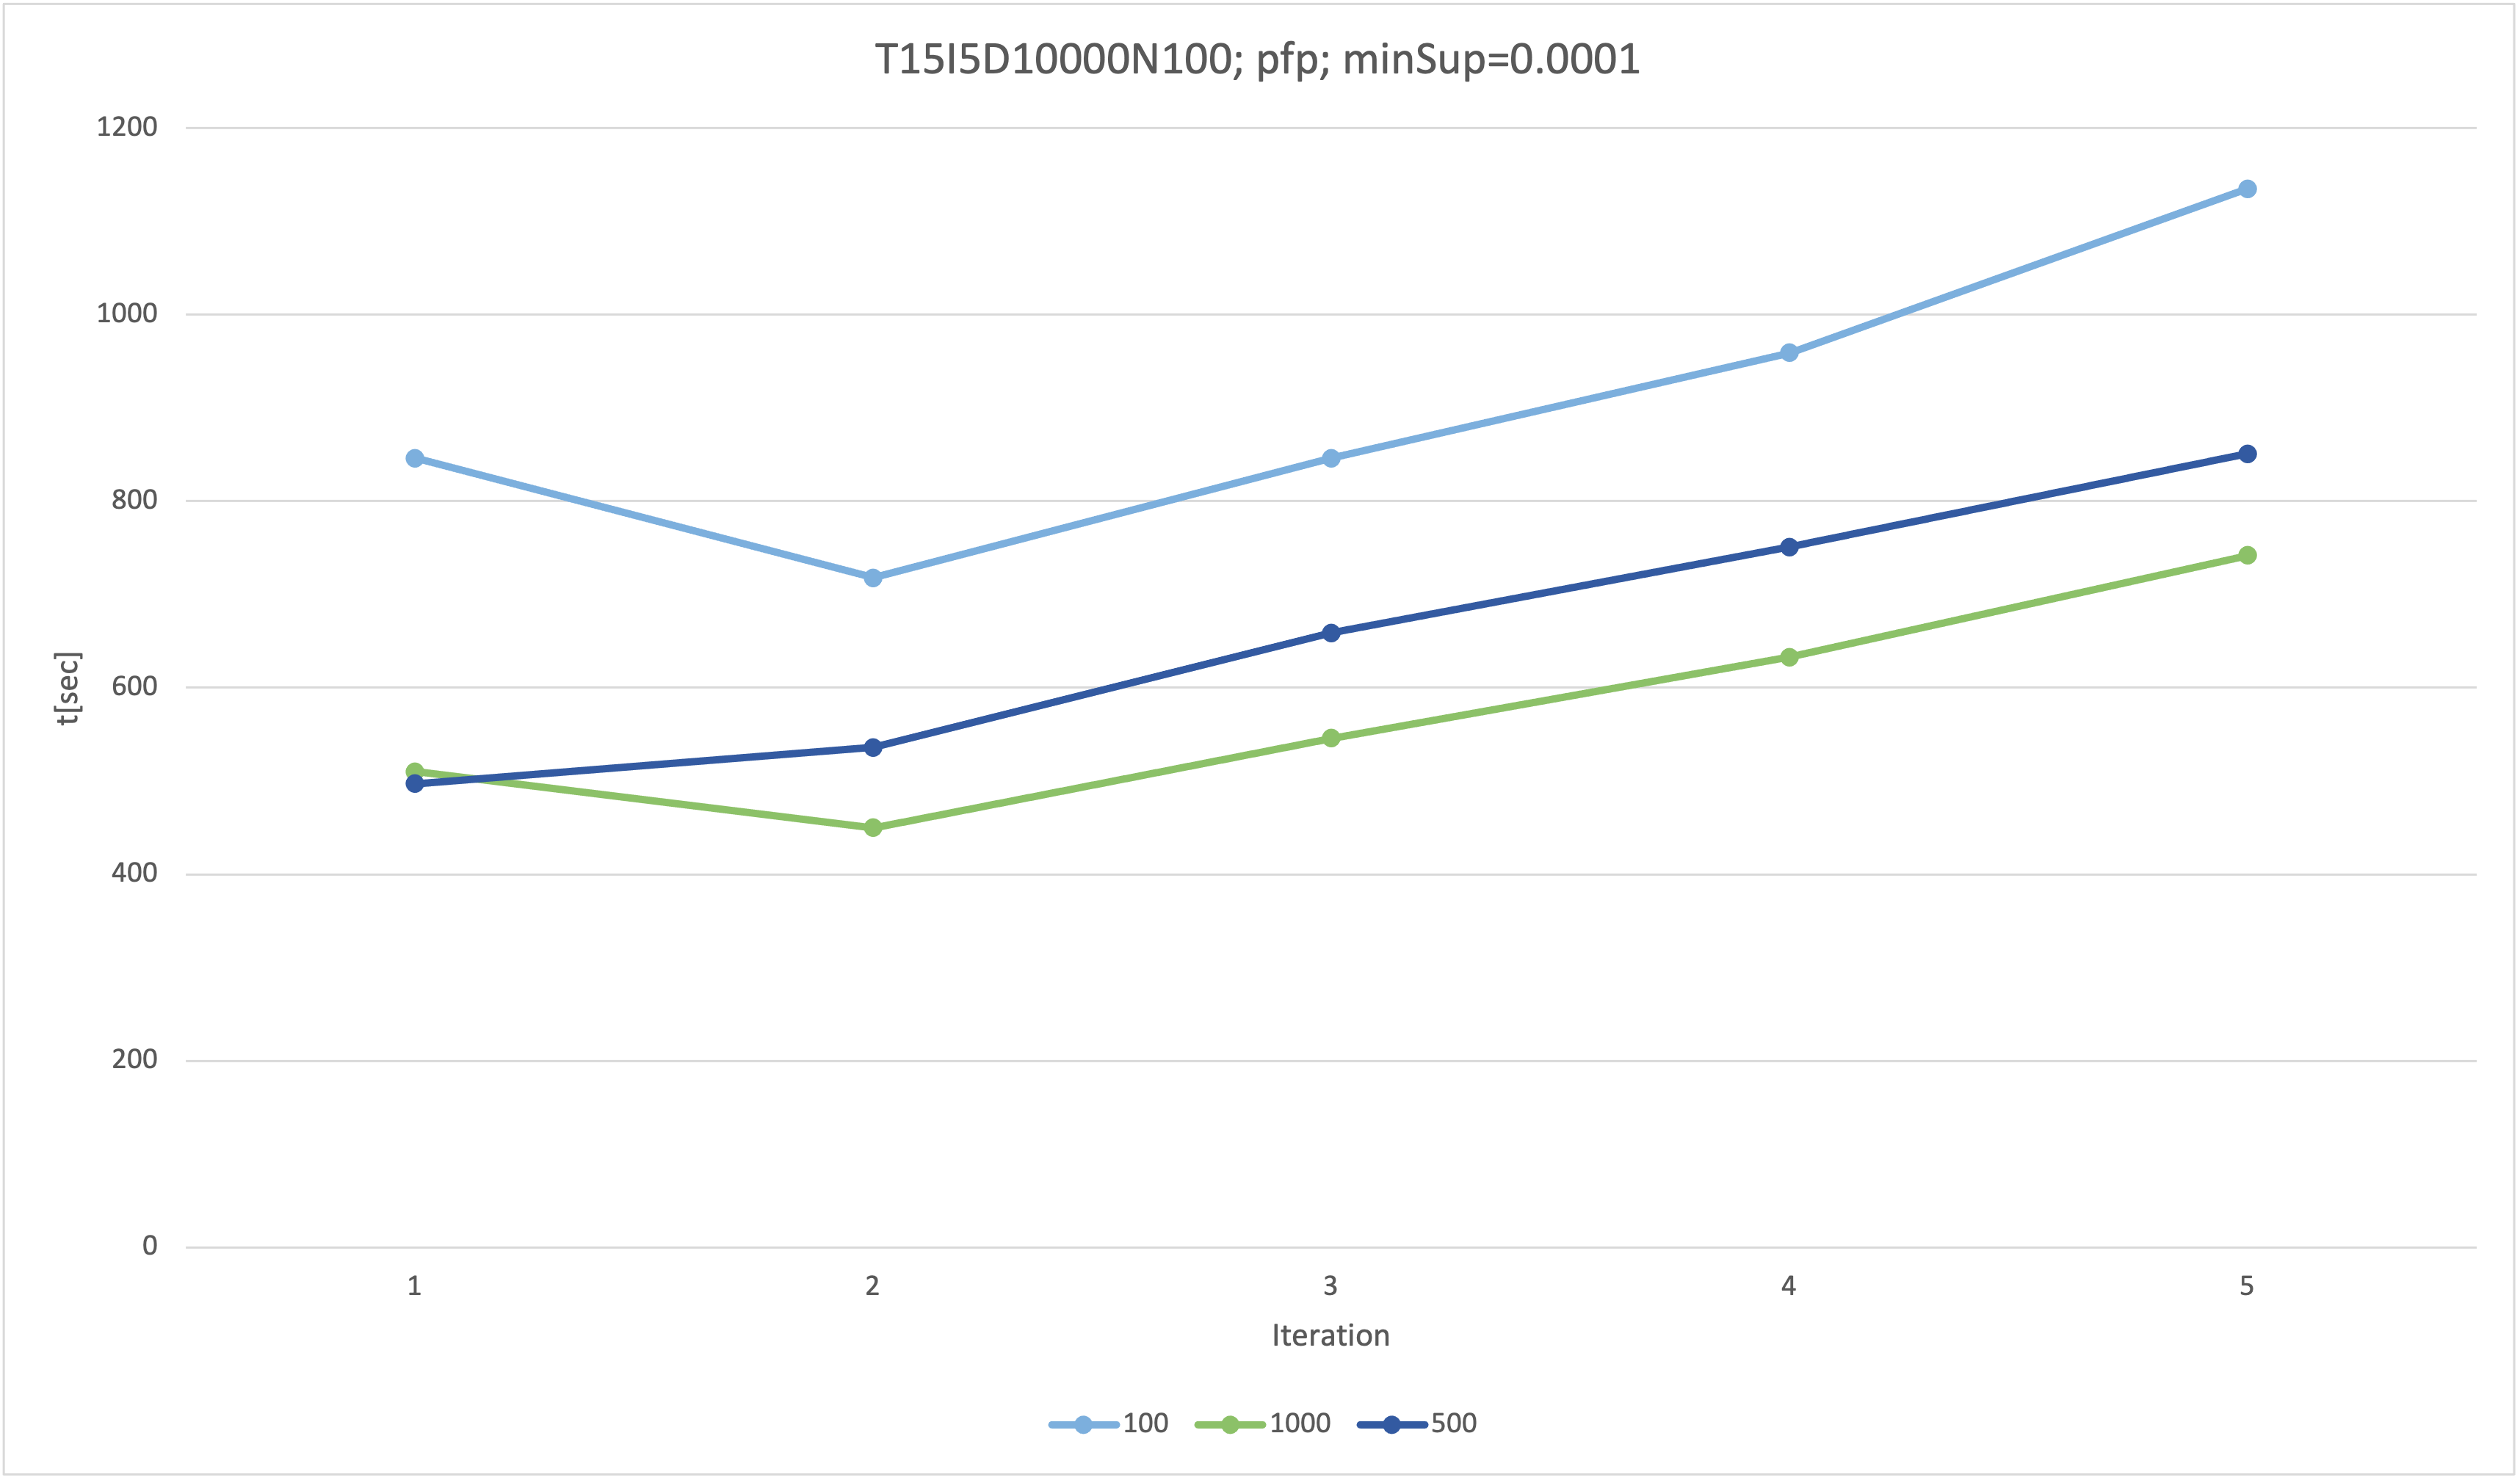
\includegraphics[width=\linewidth]{figures/4iterations/T15I5D10000N100_pfp_0001}
  \caption{T15I5D10000N100, minSup=0.0001}
  \label{fig:T15I5D10000N100_pfp_0001}
    \end{subfigure}
  \begin{subfigure}{\textwidth}
  \centering
  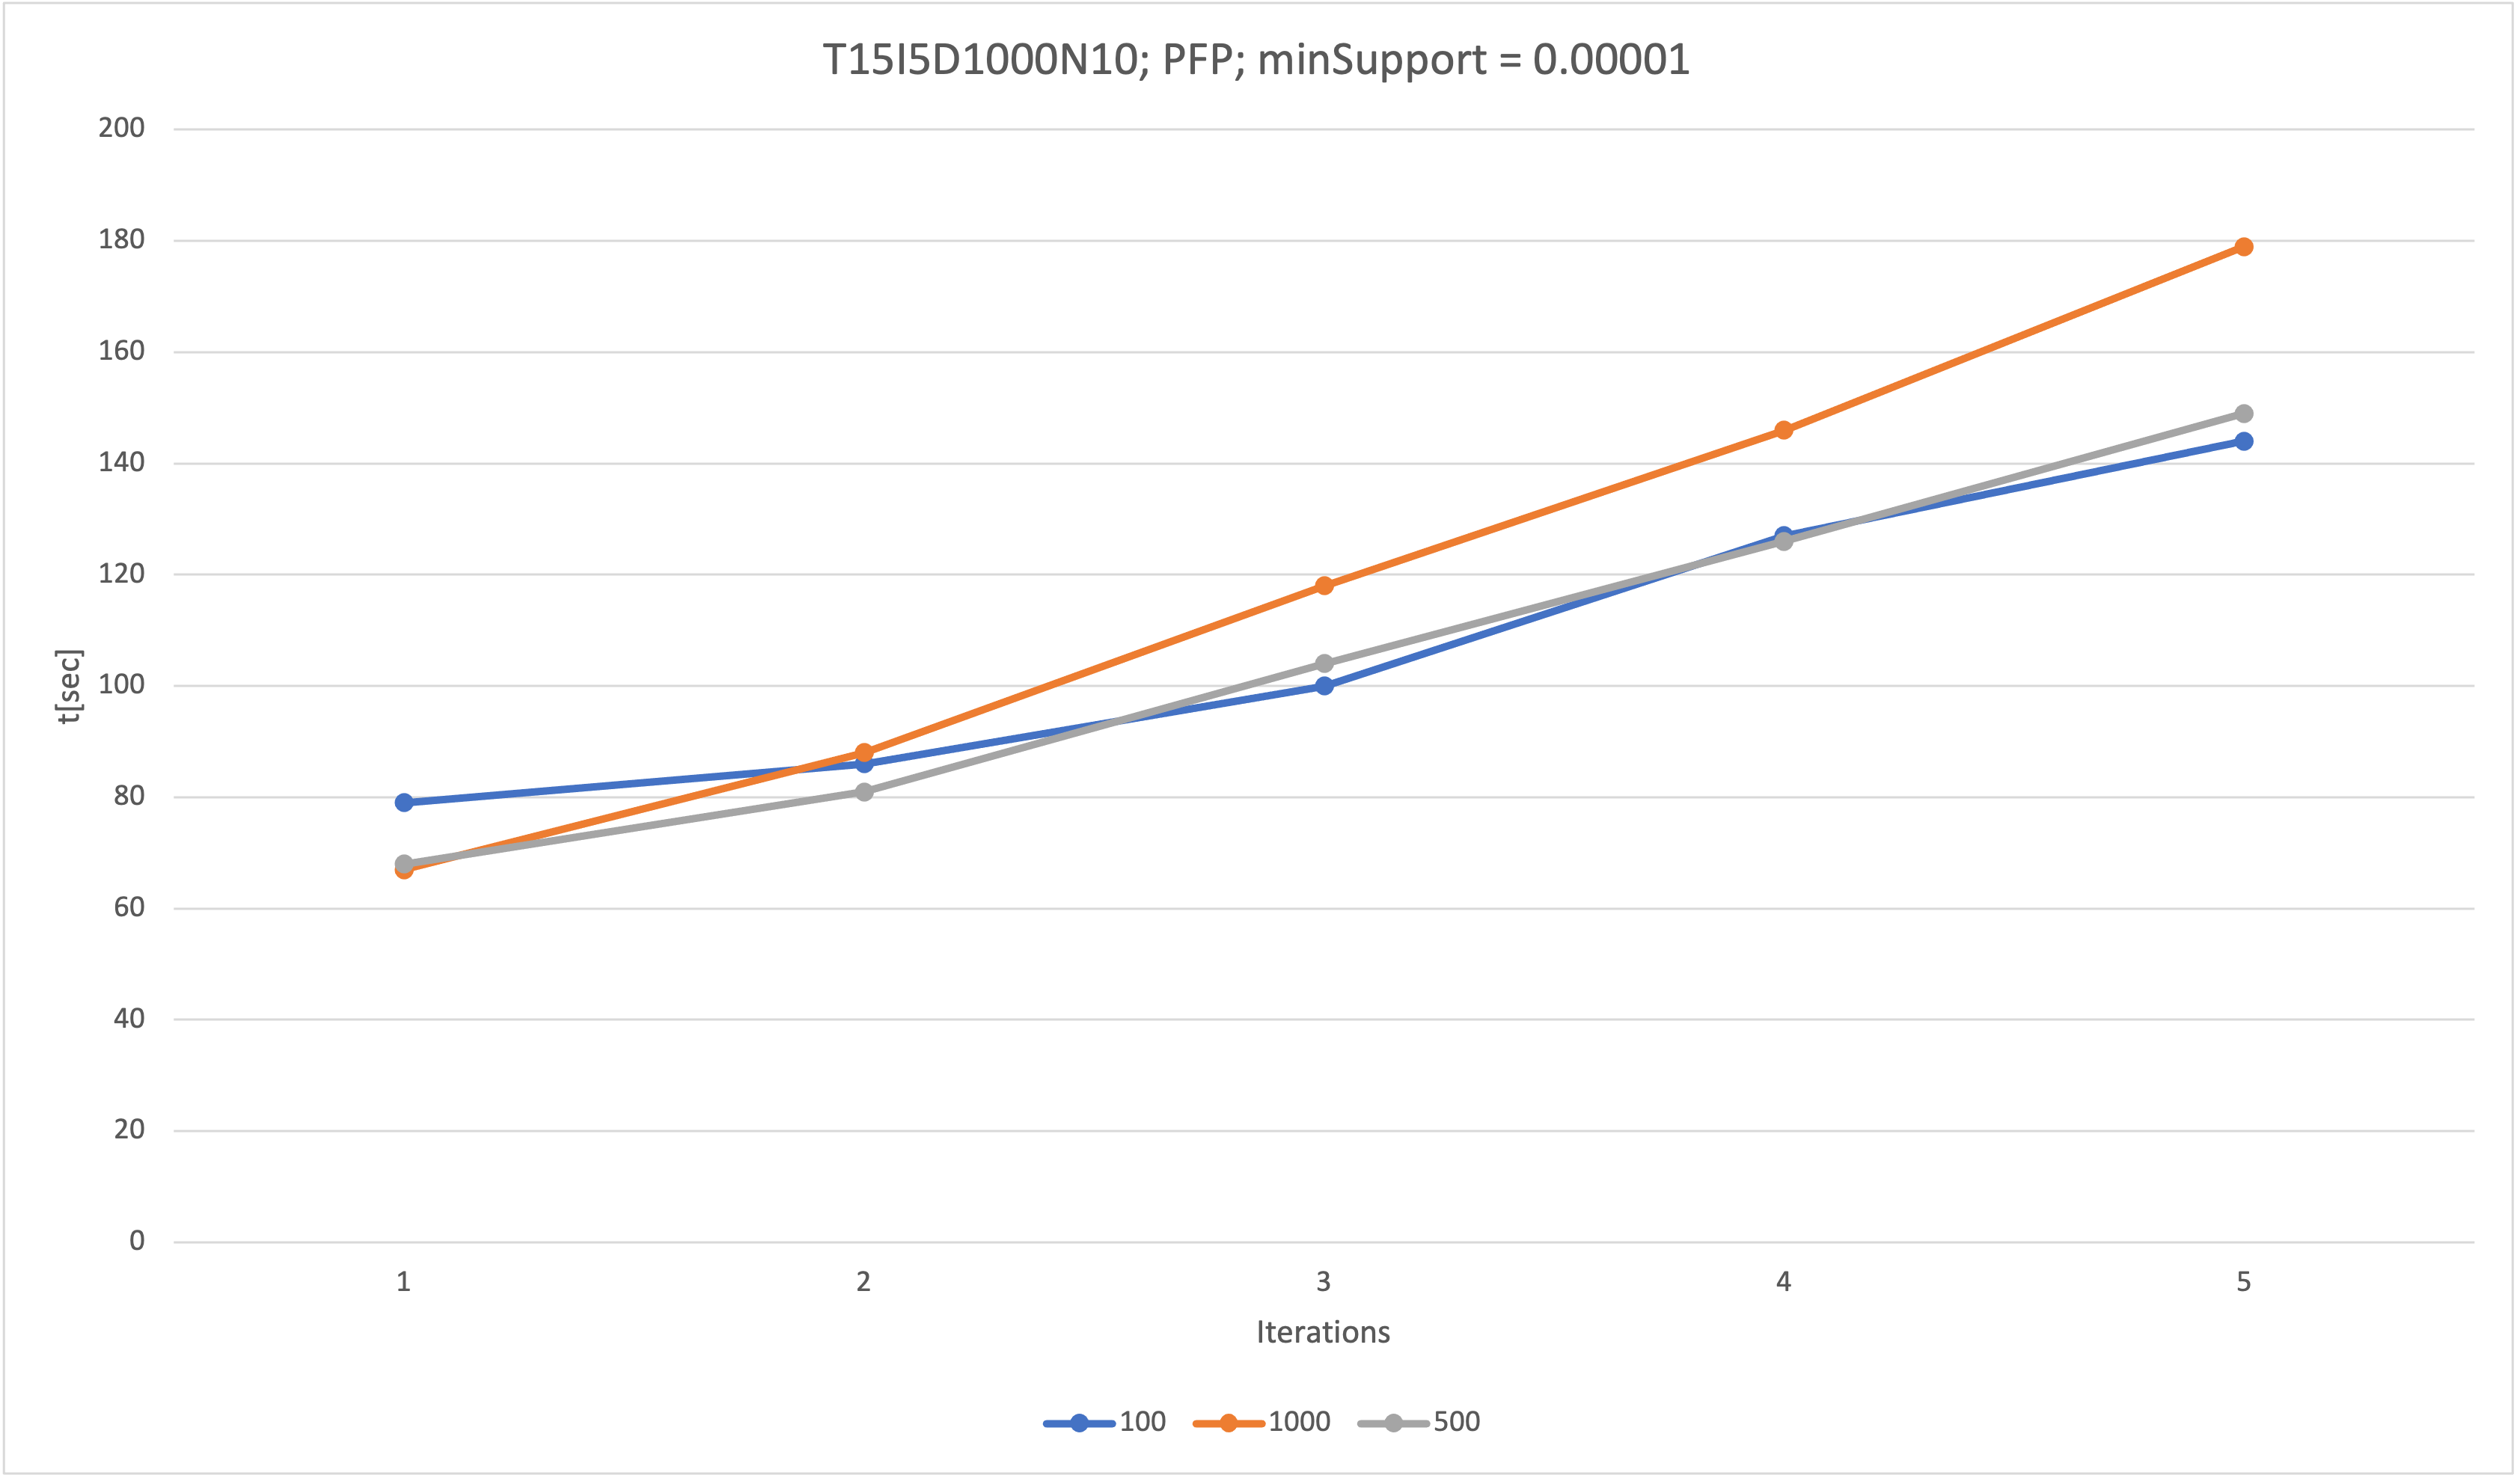
\includegraphics[width=\linewidth]{figures/4iterations/T15I5D1000N10_pfp_00001}
  \caption{T15I5D1000N10, }
  \label{fig:T15I5D1000N10_pfp_00001}
    \end{subfigure}
    \caption{PFP, 100\textbar 1000\textbar 500 partitions}
\end{figure}


\paragraph{Song}
~\autoref{fig:kosarak_song_001} presents Song performance on ~\autoref{data:kosarak}. Best performance is achieved for 100 and 1000 partitions. ~\autoref{fig:T15I5D10000N100_song_0001} presents Song on ~\autoref{data:10Msynt} with minSupport = 1e-05. The run failed for 100 partitions due to memory error. Best performance achieved for 500 partitions.
~\autoref{fig:T15I5D1000N10_song_00001} presents Song on ~\autoref{data:1Msynt}, best performance achieved for 1000 partitions.


\begin{figure}[H]
  \centering
  \begin{subfigure}{\textwidth}
	  \centering
 	 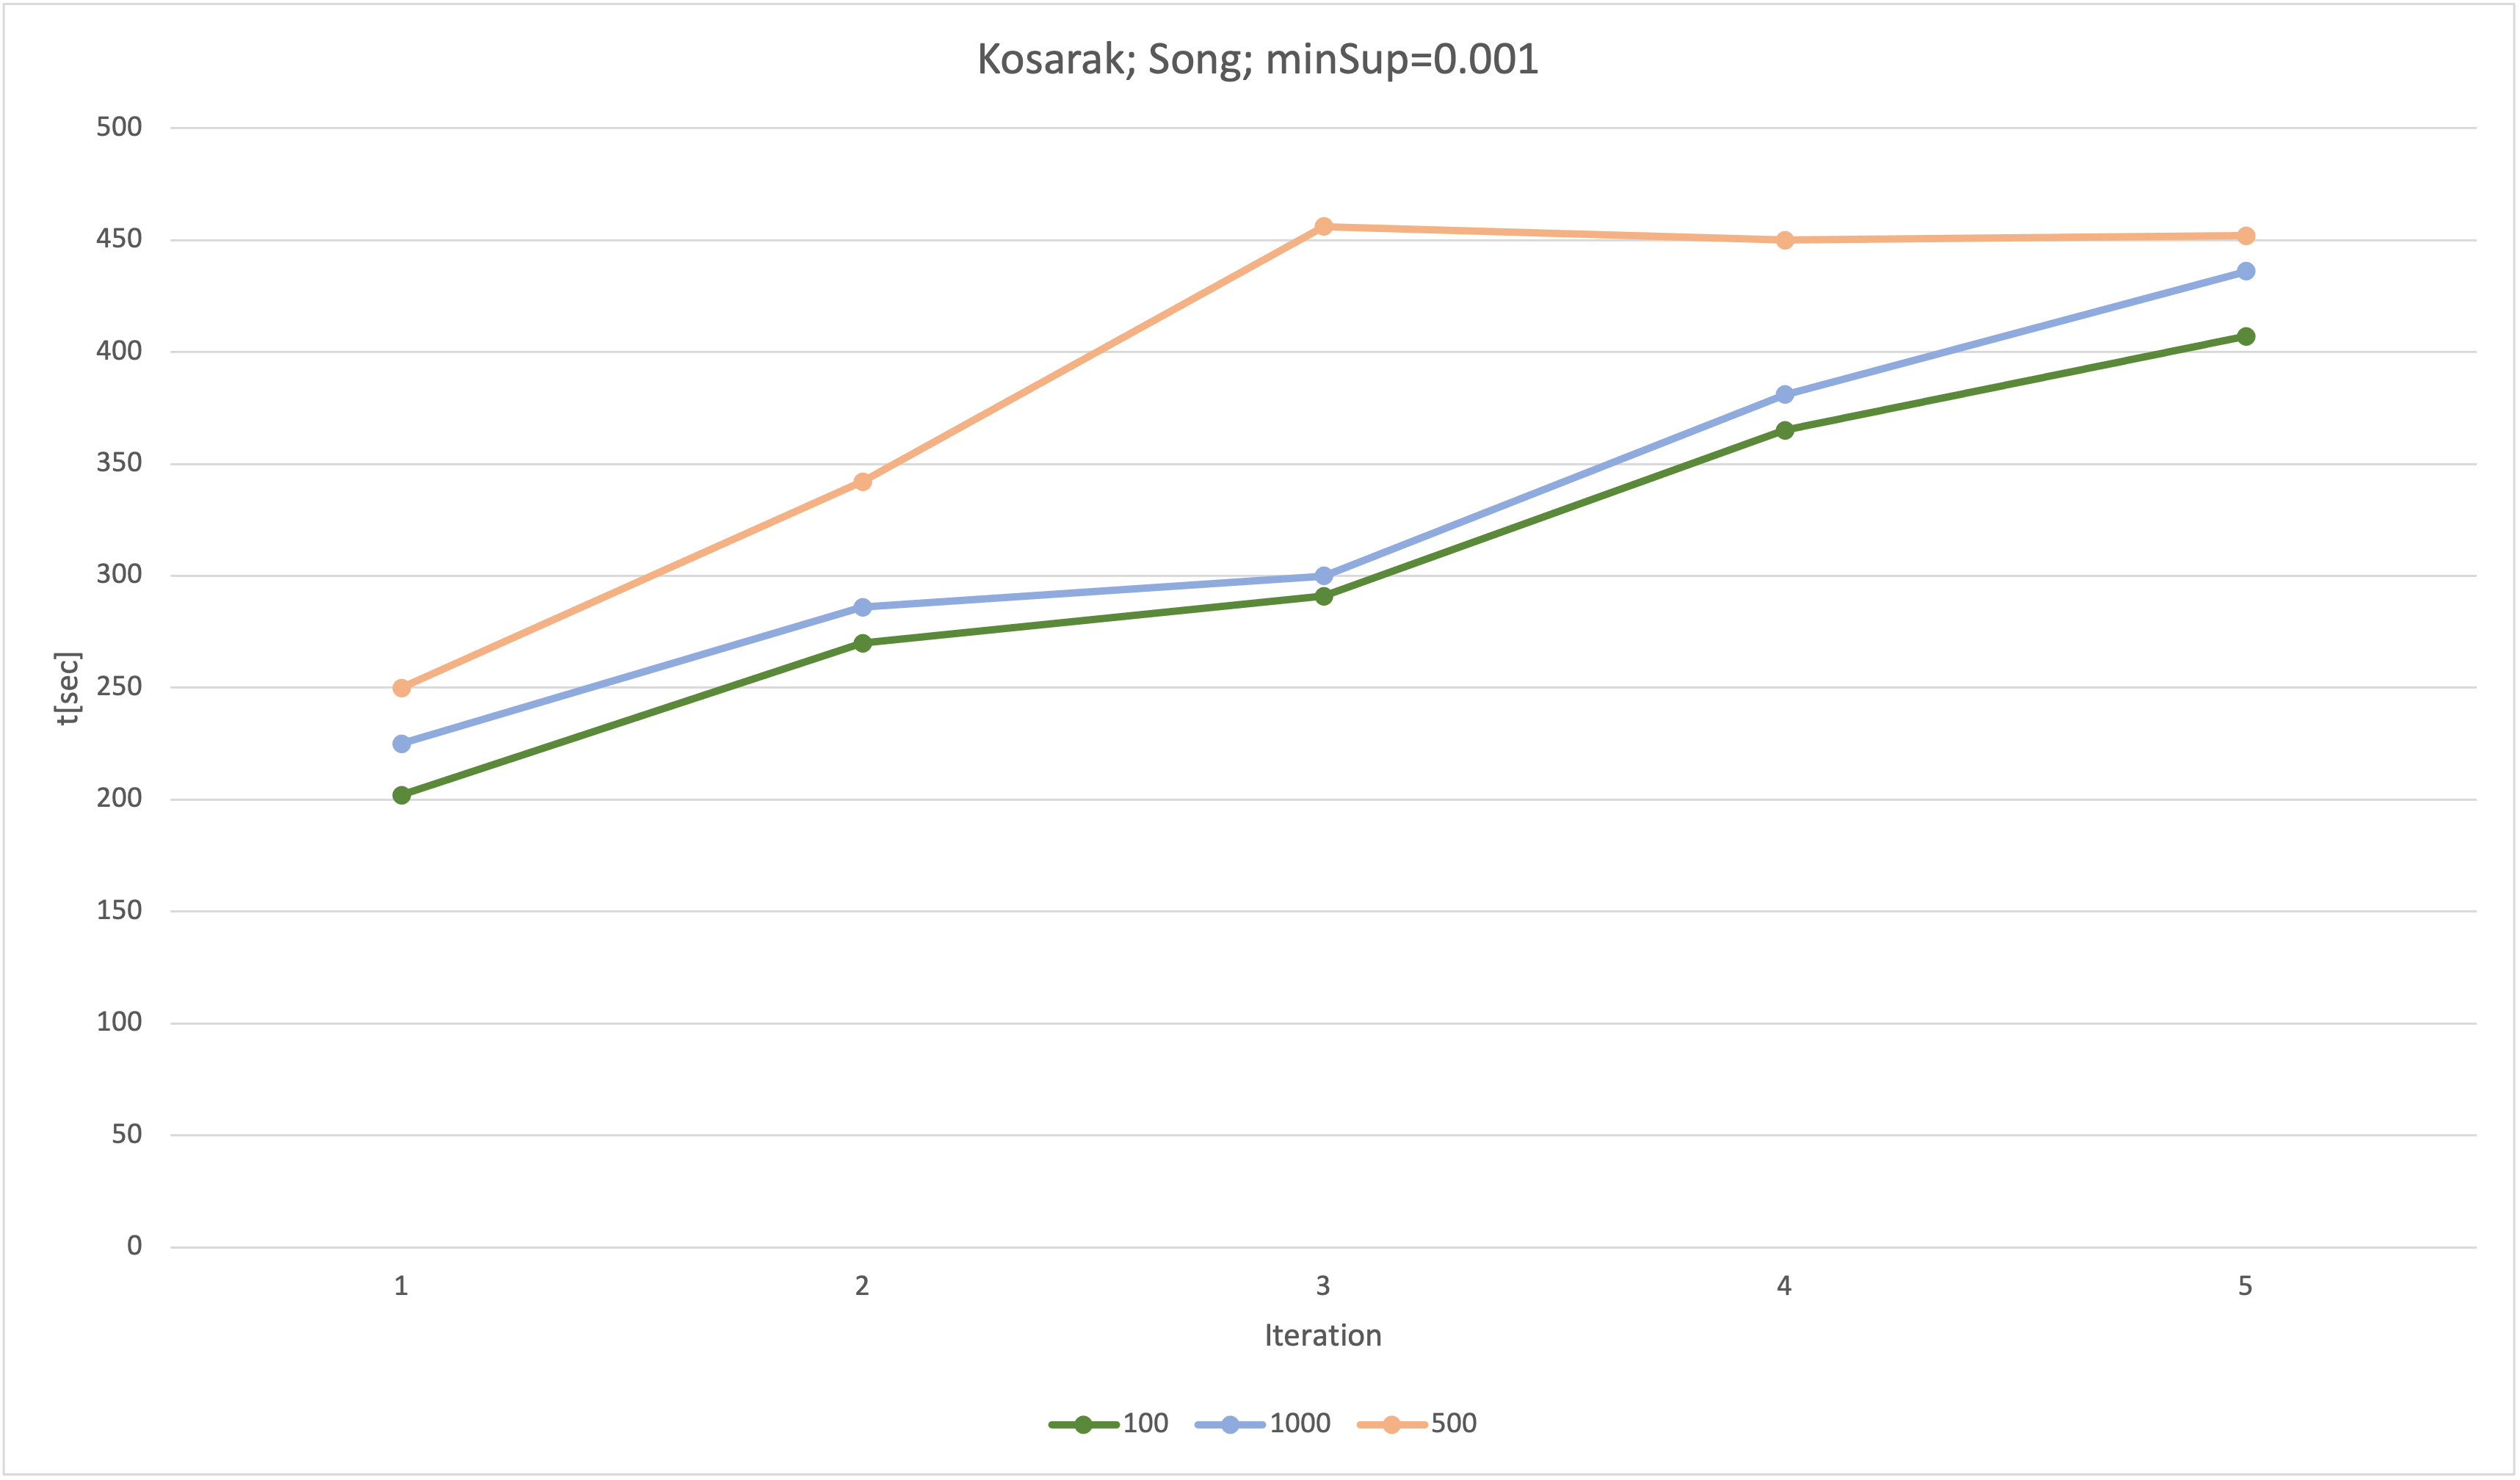
\includegraphics[width=\linewidth]{figures/4iterations/kosarak_song_001}
	  \caption{kosarak, minSup = 0.001}
	  \label{fig:kosarak_song_001}
  \end{subfigure}
  \begin{subfigure}{\textwidth}
    \centering
	  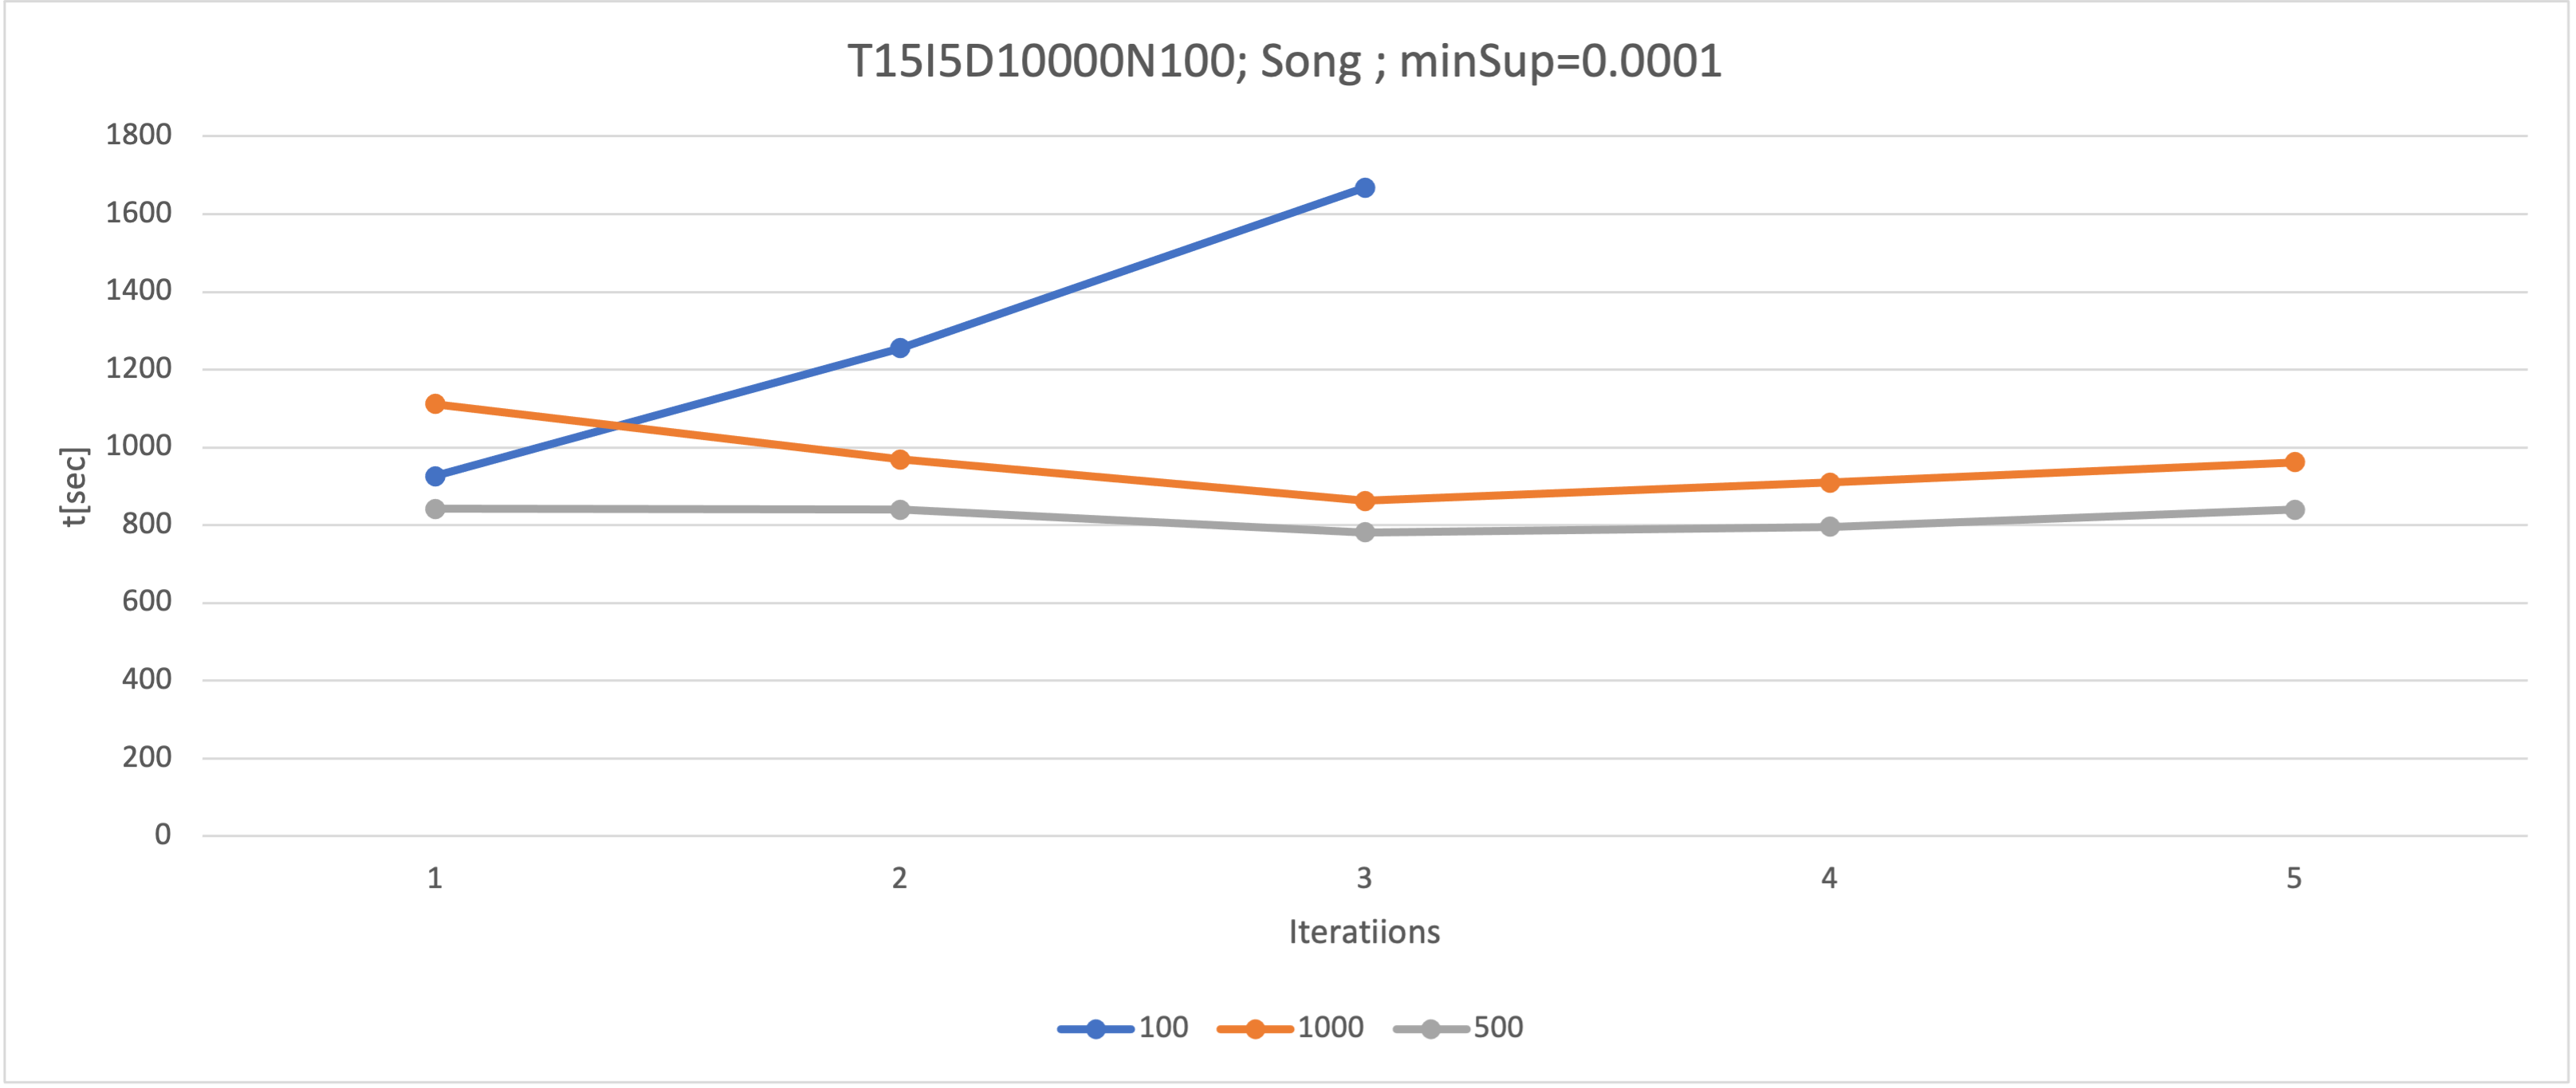
\includegraphics[width=\linewidth]{figures/4iterations/T15I5D10000N100_song_0001}
	  \caption{T15I5D10000N100 Song, minSup = 0.0001}
	  \label{fig:T15I5D10000N100_song_0001}
  \end{subfigure}  
    \begin{subfigure}{\textwidth}
	    \centering
	  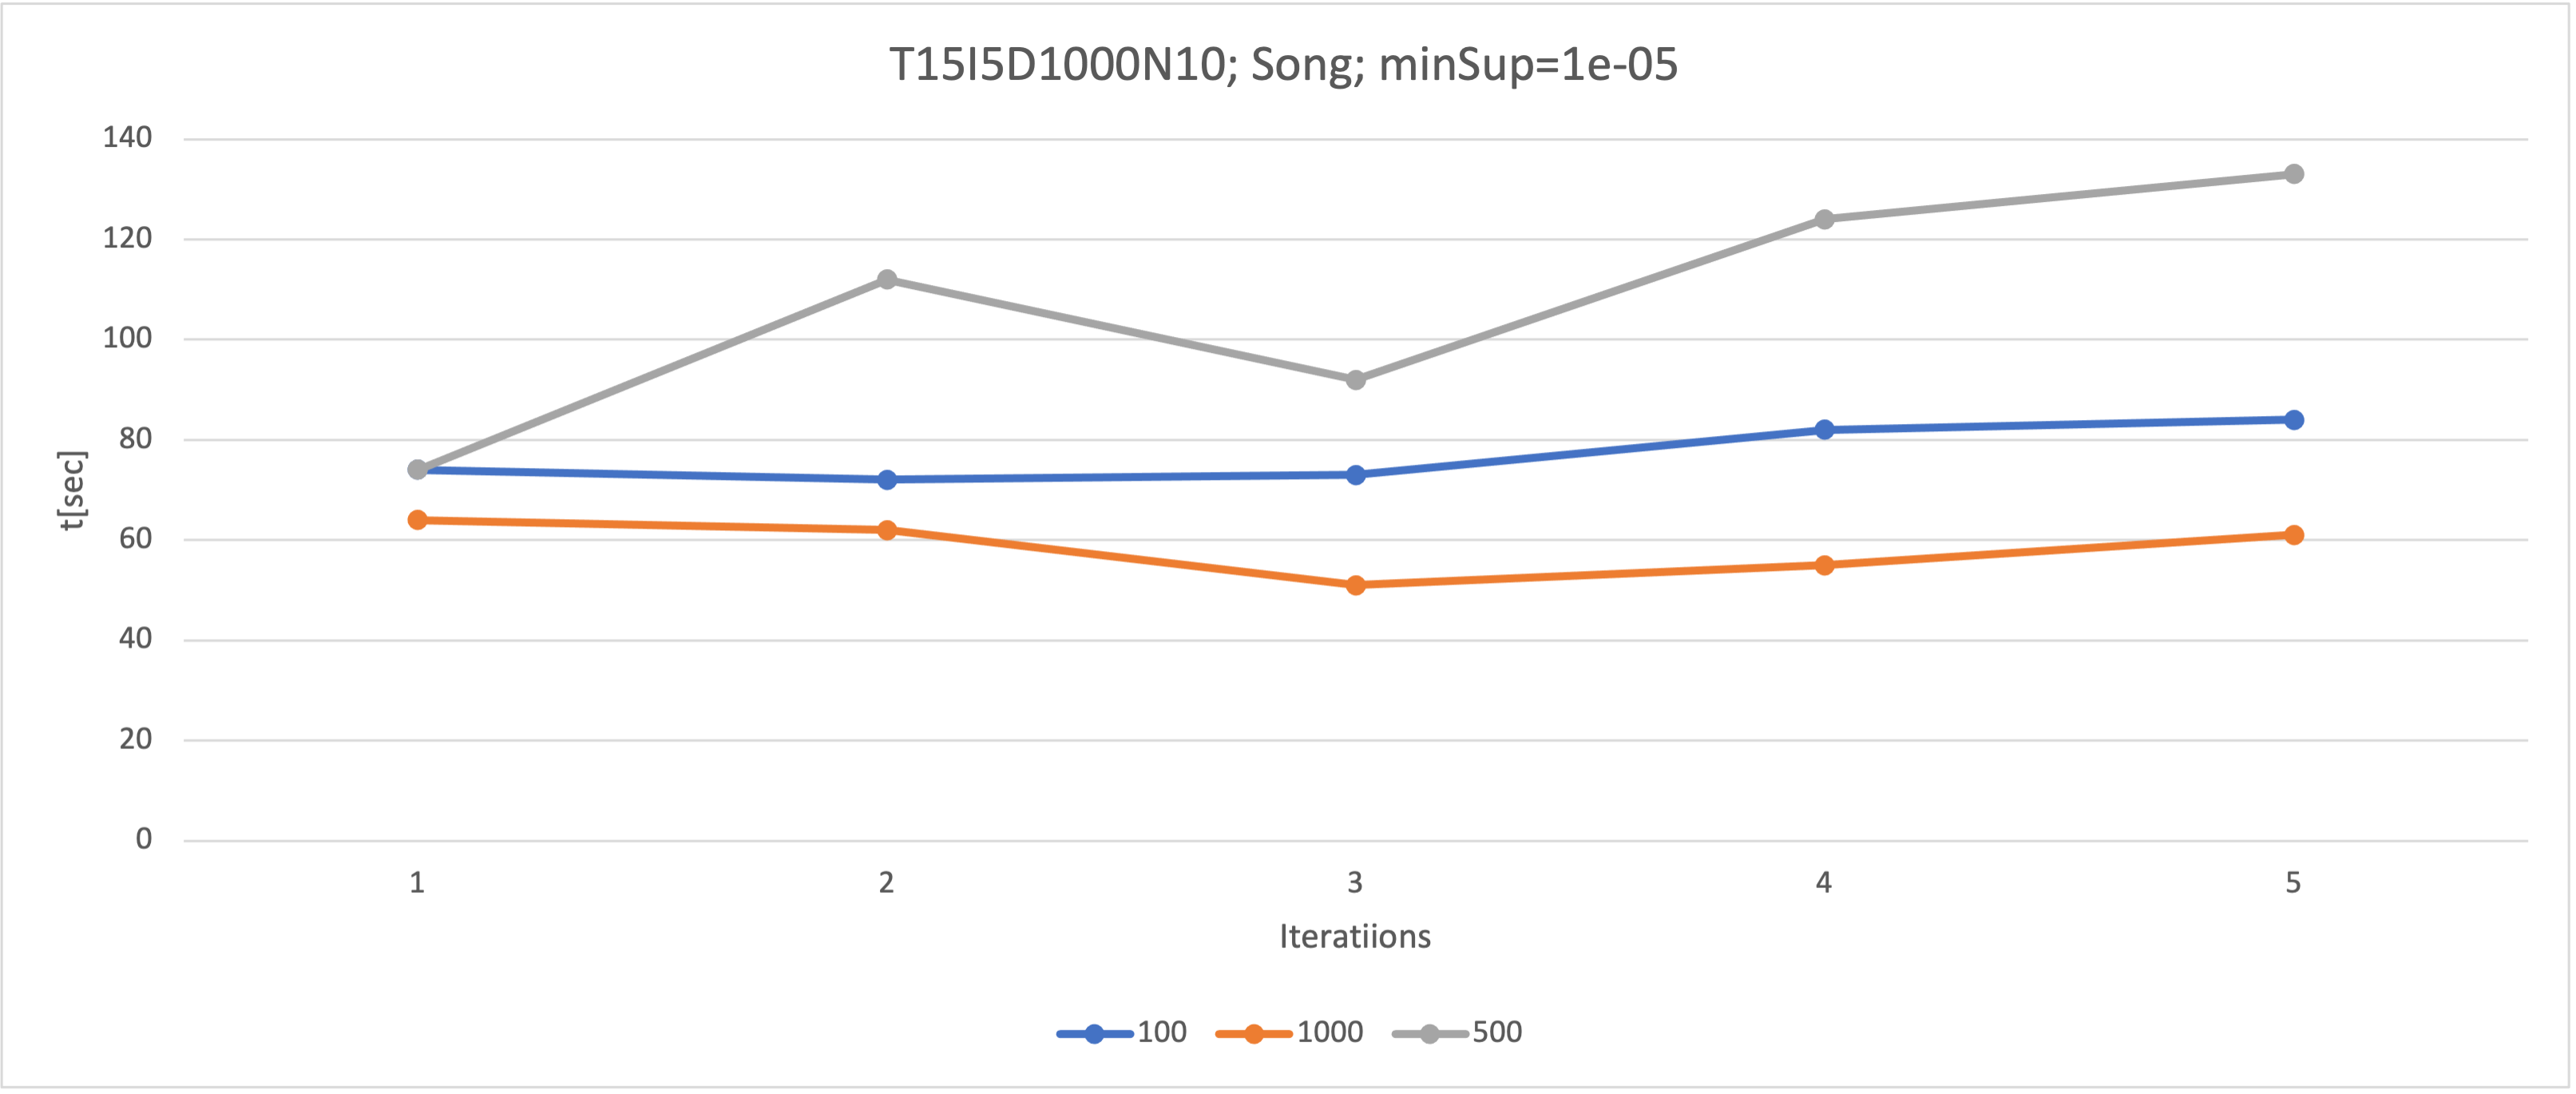
\includegraphics[width=\linewidth]{figures/4iterations/T15I5D1000N10_song_00001}
	  \caption{T15I5D1000N10 Song, minSup = 1e-05}
	  \label{fig:T15I5D1000N10_song_00001}
  \end{subfigure}  
  \caption{SONG 100\textbar 1000\textbar 500 partitions}
\end{figure}

\paragraph{IPFIM}
~\autoref{fig:T15I5D10000N100_ipfim_0001} presents IPFIM on ~\autoref{data:10Msynt}.  Best performance achieved on 1000 partitions. 

\begin{figure}[H]
  \centering
  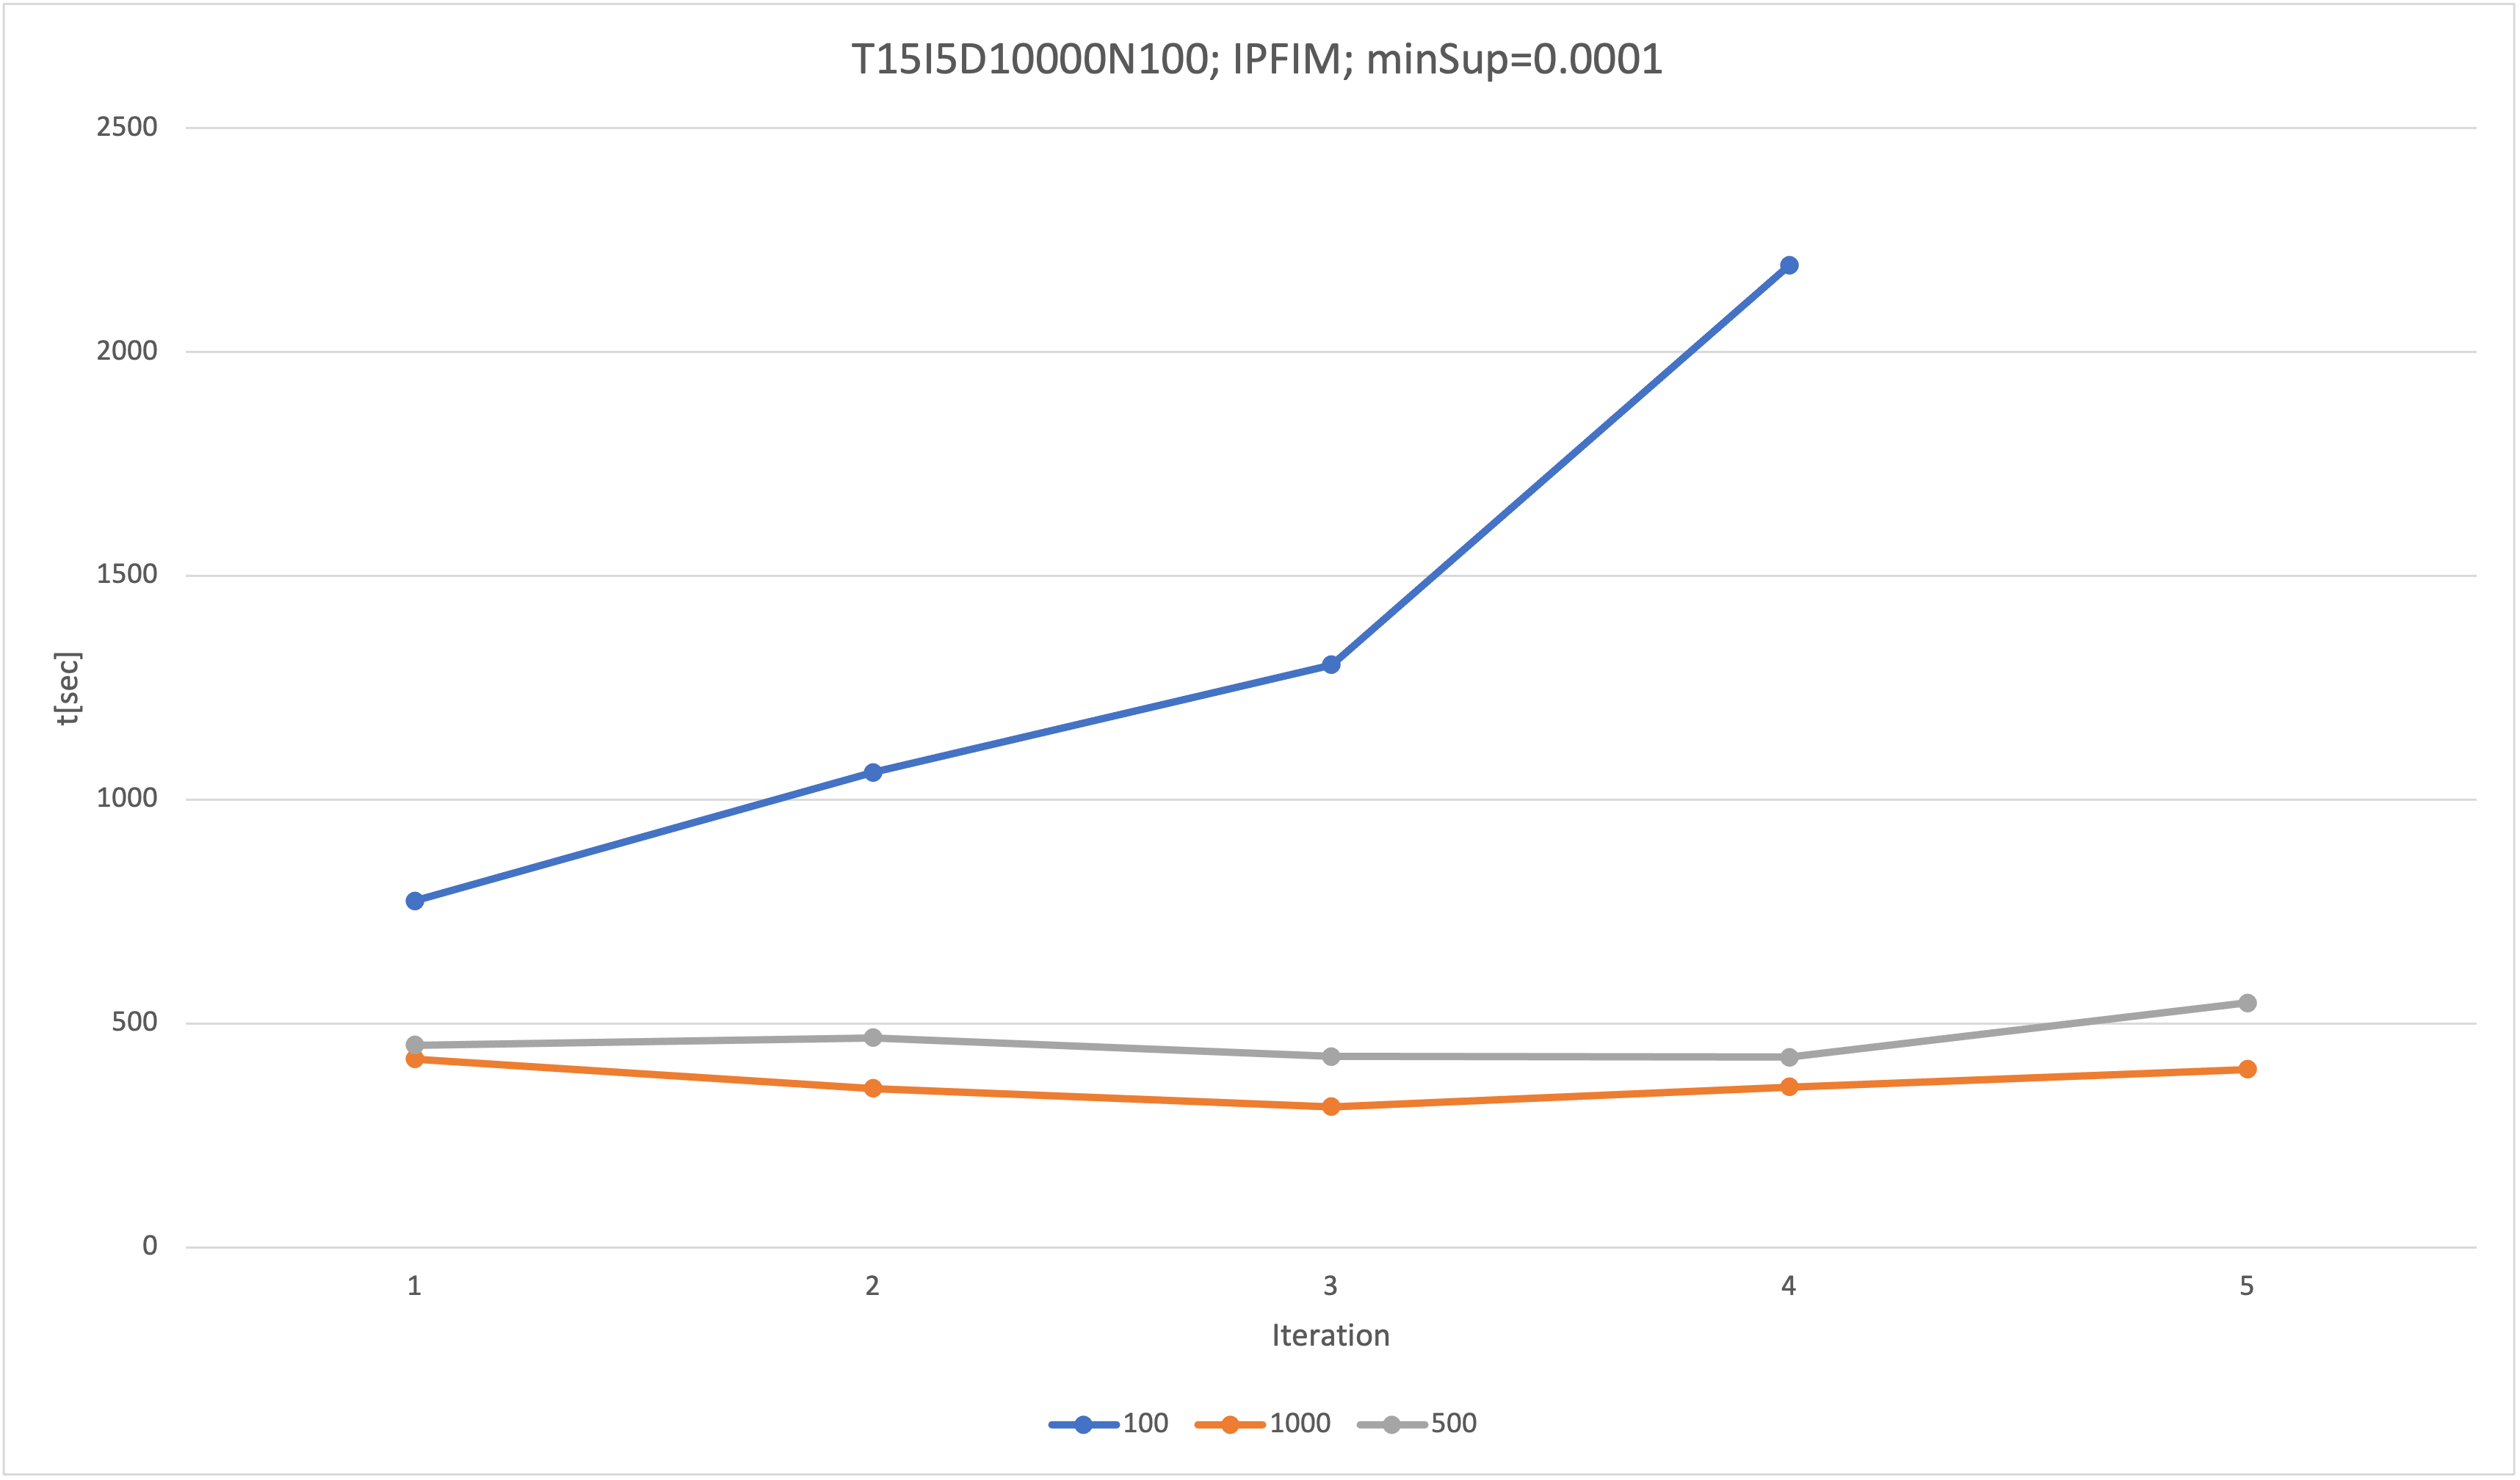
\includegraphics[width=\linewidth]{figures/4iterations/T15I5D10000N100_ipfim_0001}
  \caption{T15I5D10000N100, minSup = 0.0001,  IPFIM 100\textbar 1000\textbar 500 partitions}
  \label{fig:T15I5D10000N100_ipfim_0001}
\end{figure}


\paragraph{IPFIM Improved}
~\autoref{fig:kosarak_ipfim_imp_001} presents IPFIM improved on ~\autoref{data:kosarak}.  Best performance achieved on 1000 partitions.  ~\autoref{fig:T15I5D10000N100_ipfim_imp_0001} presents IPFIM improved ~\autoref{data:10Msynt}.  Best performance achieved on 1000 partitions. \autoref{fig:T15I5D1000N10_ipfim_imp_00001} presents IPFIM improved ~\autoref{data:1Msynt}.  Best performance achieved on 1000 partitions. 

\begin{figure}[H]
  \centering
  \begin{subfigure}{\textwidth}
  \centering
  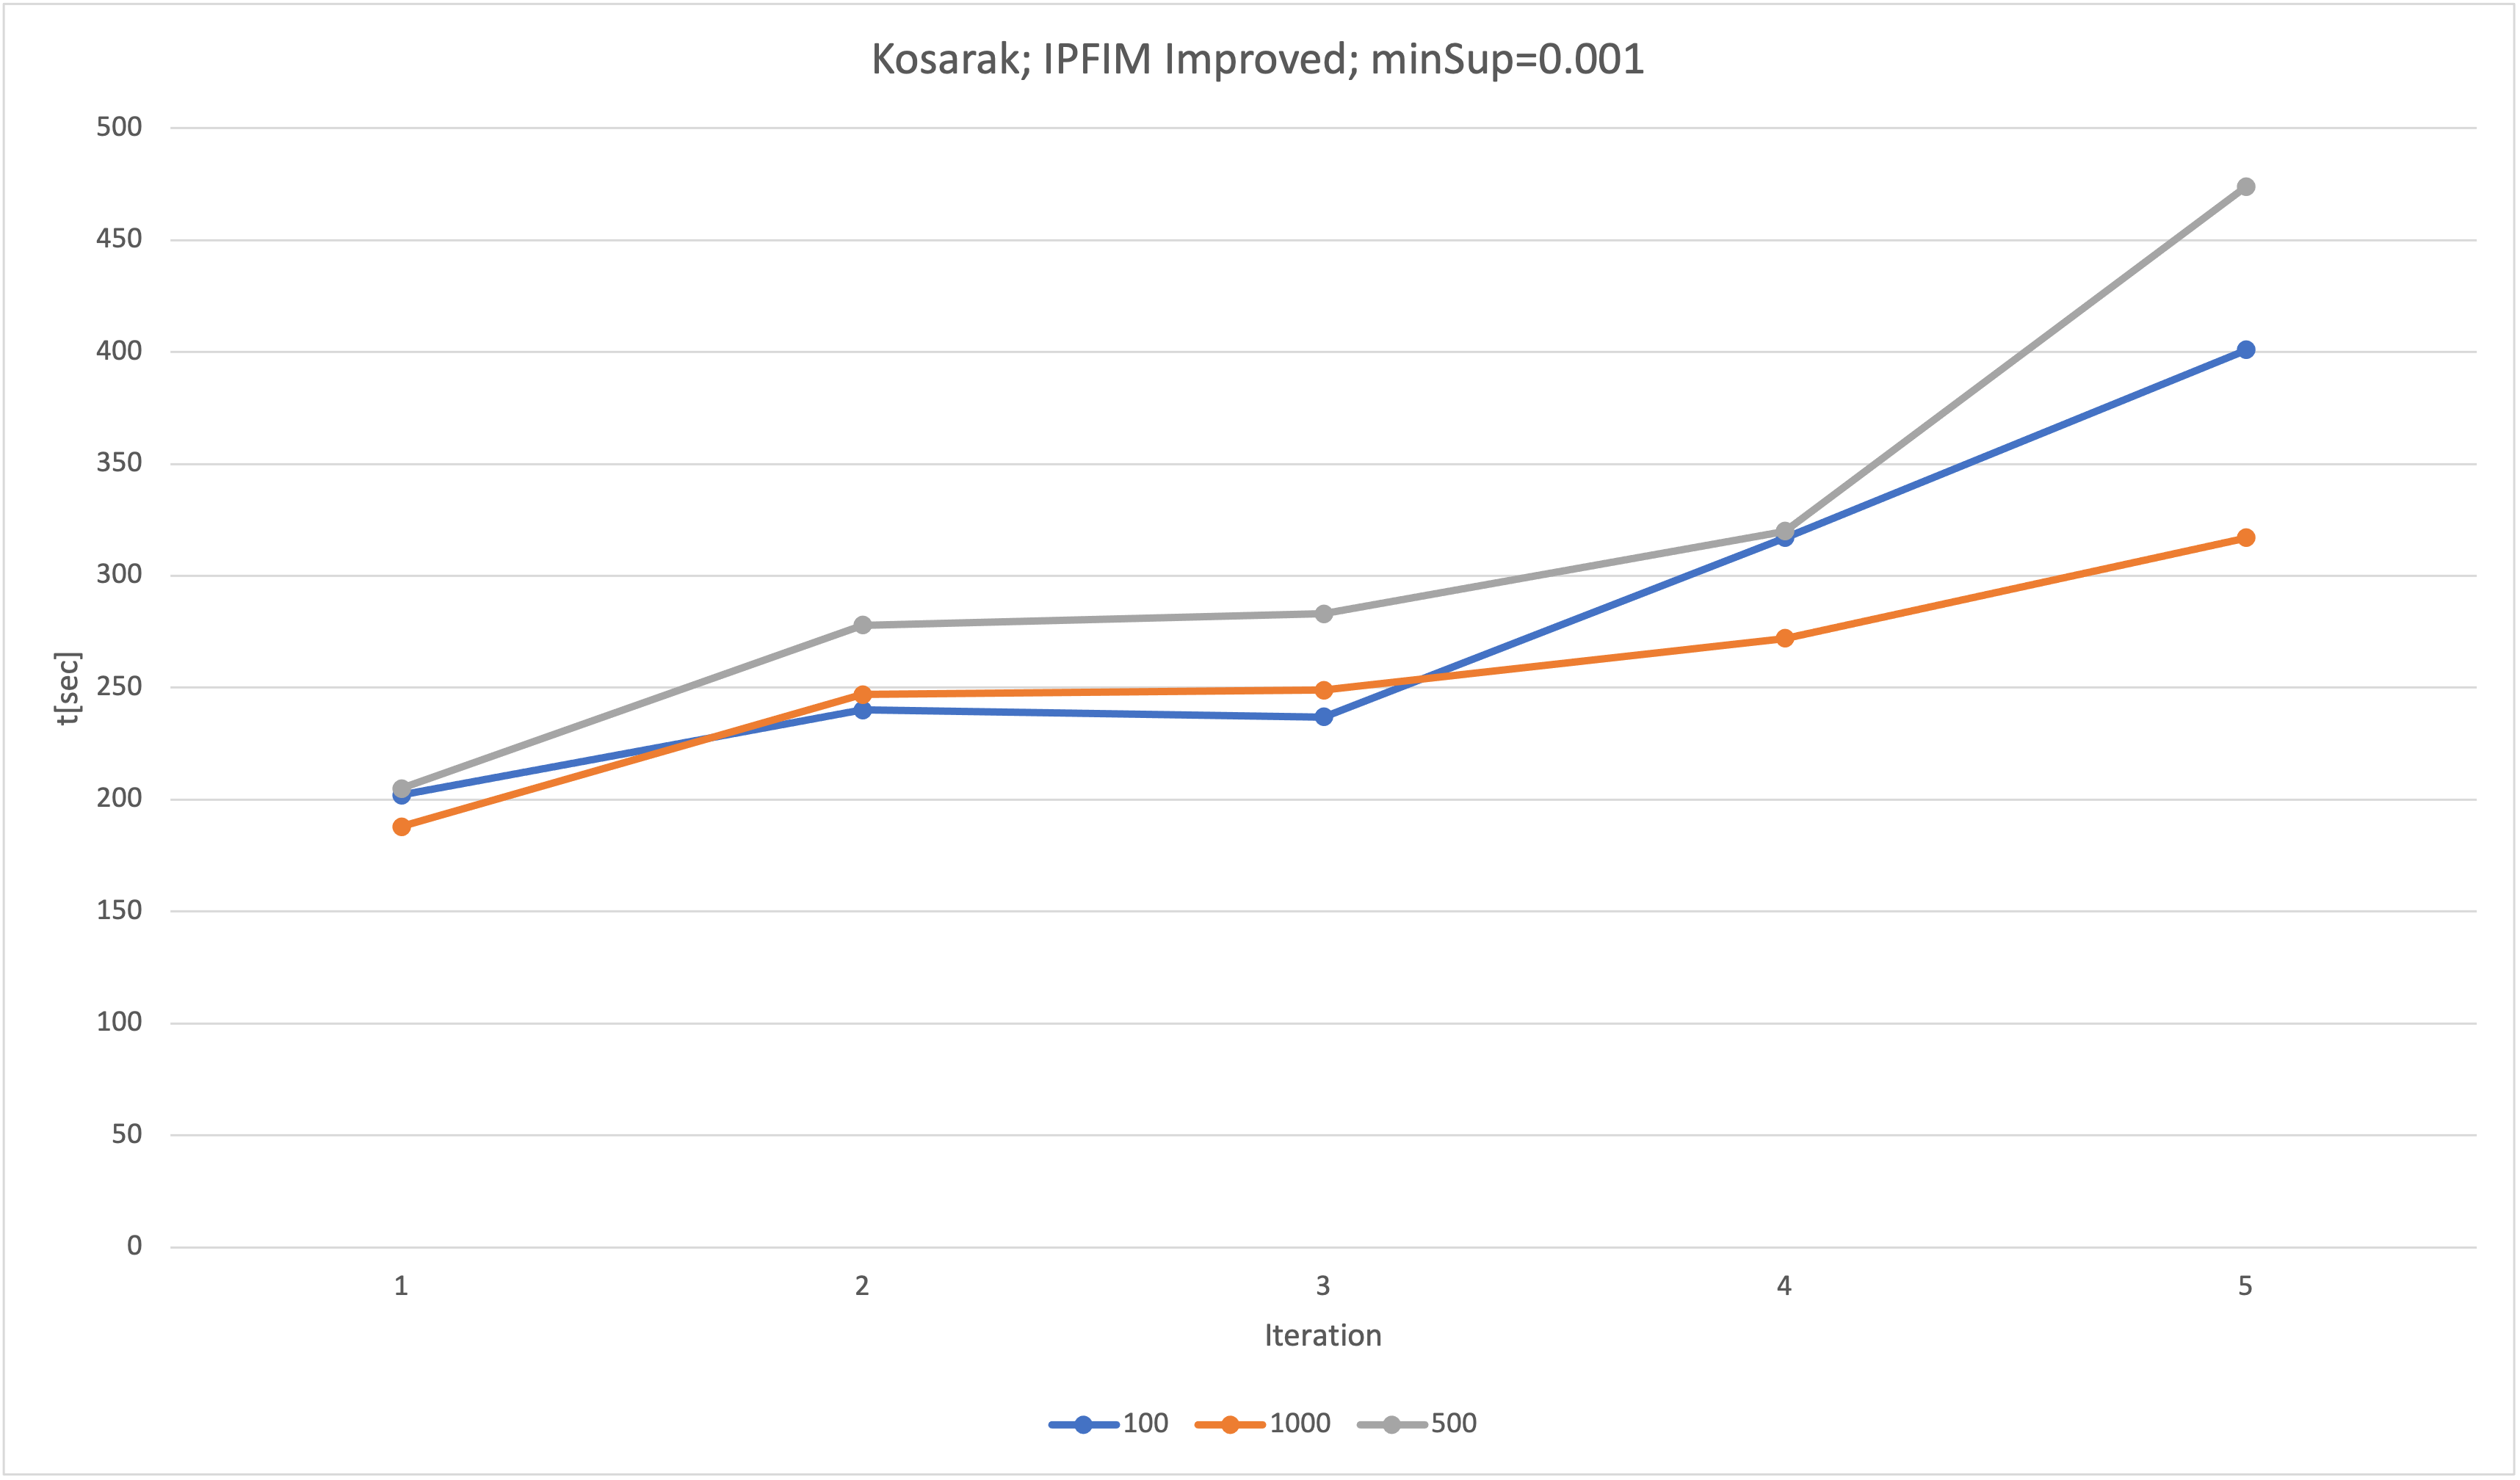
\includegraphics[width=\linewidth]{figures/4iterations/kosarak_ipfim_imp_001}
  \caption{kosarak, minSup = 0.001,  minMinSup = 0.1}
  \label{fig:kosarak_ipfim_imp_001}
    \end{subfigure}  
  \begin{subfigure}{\textwidth}
    \centering
  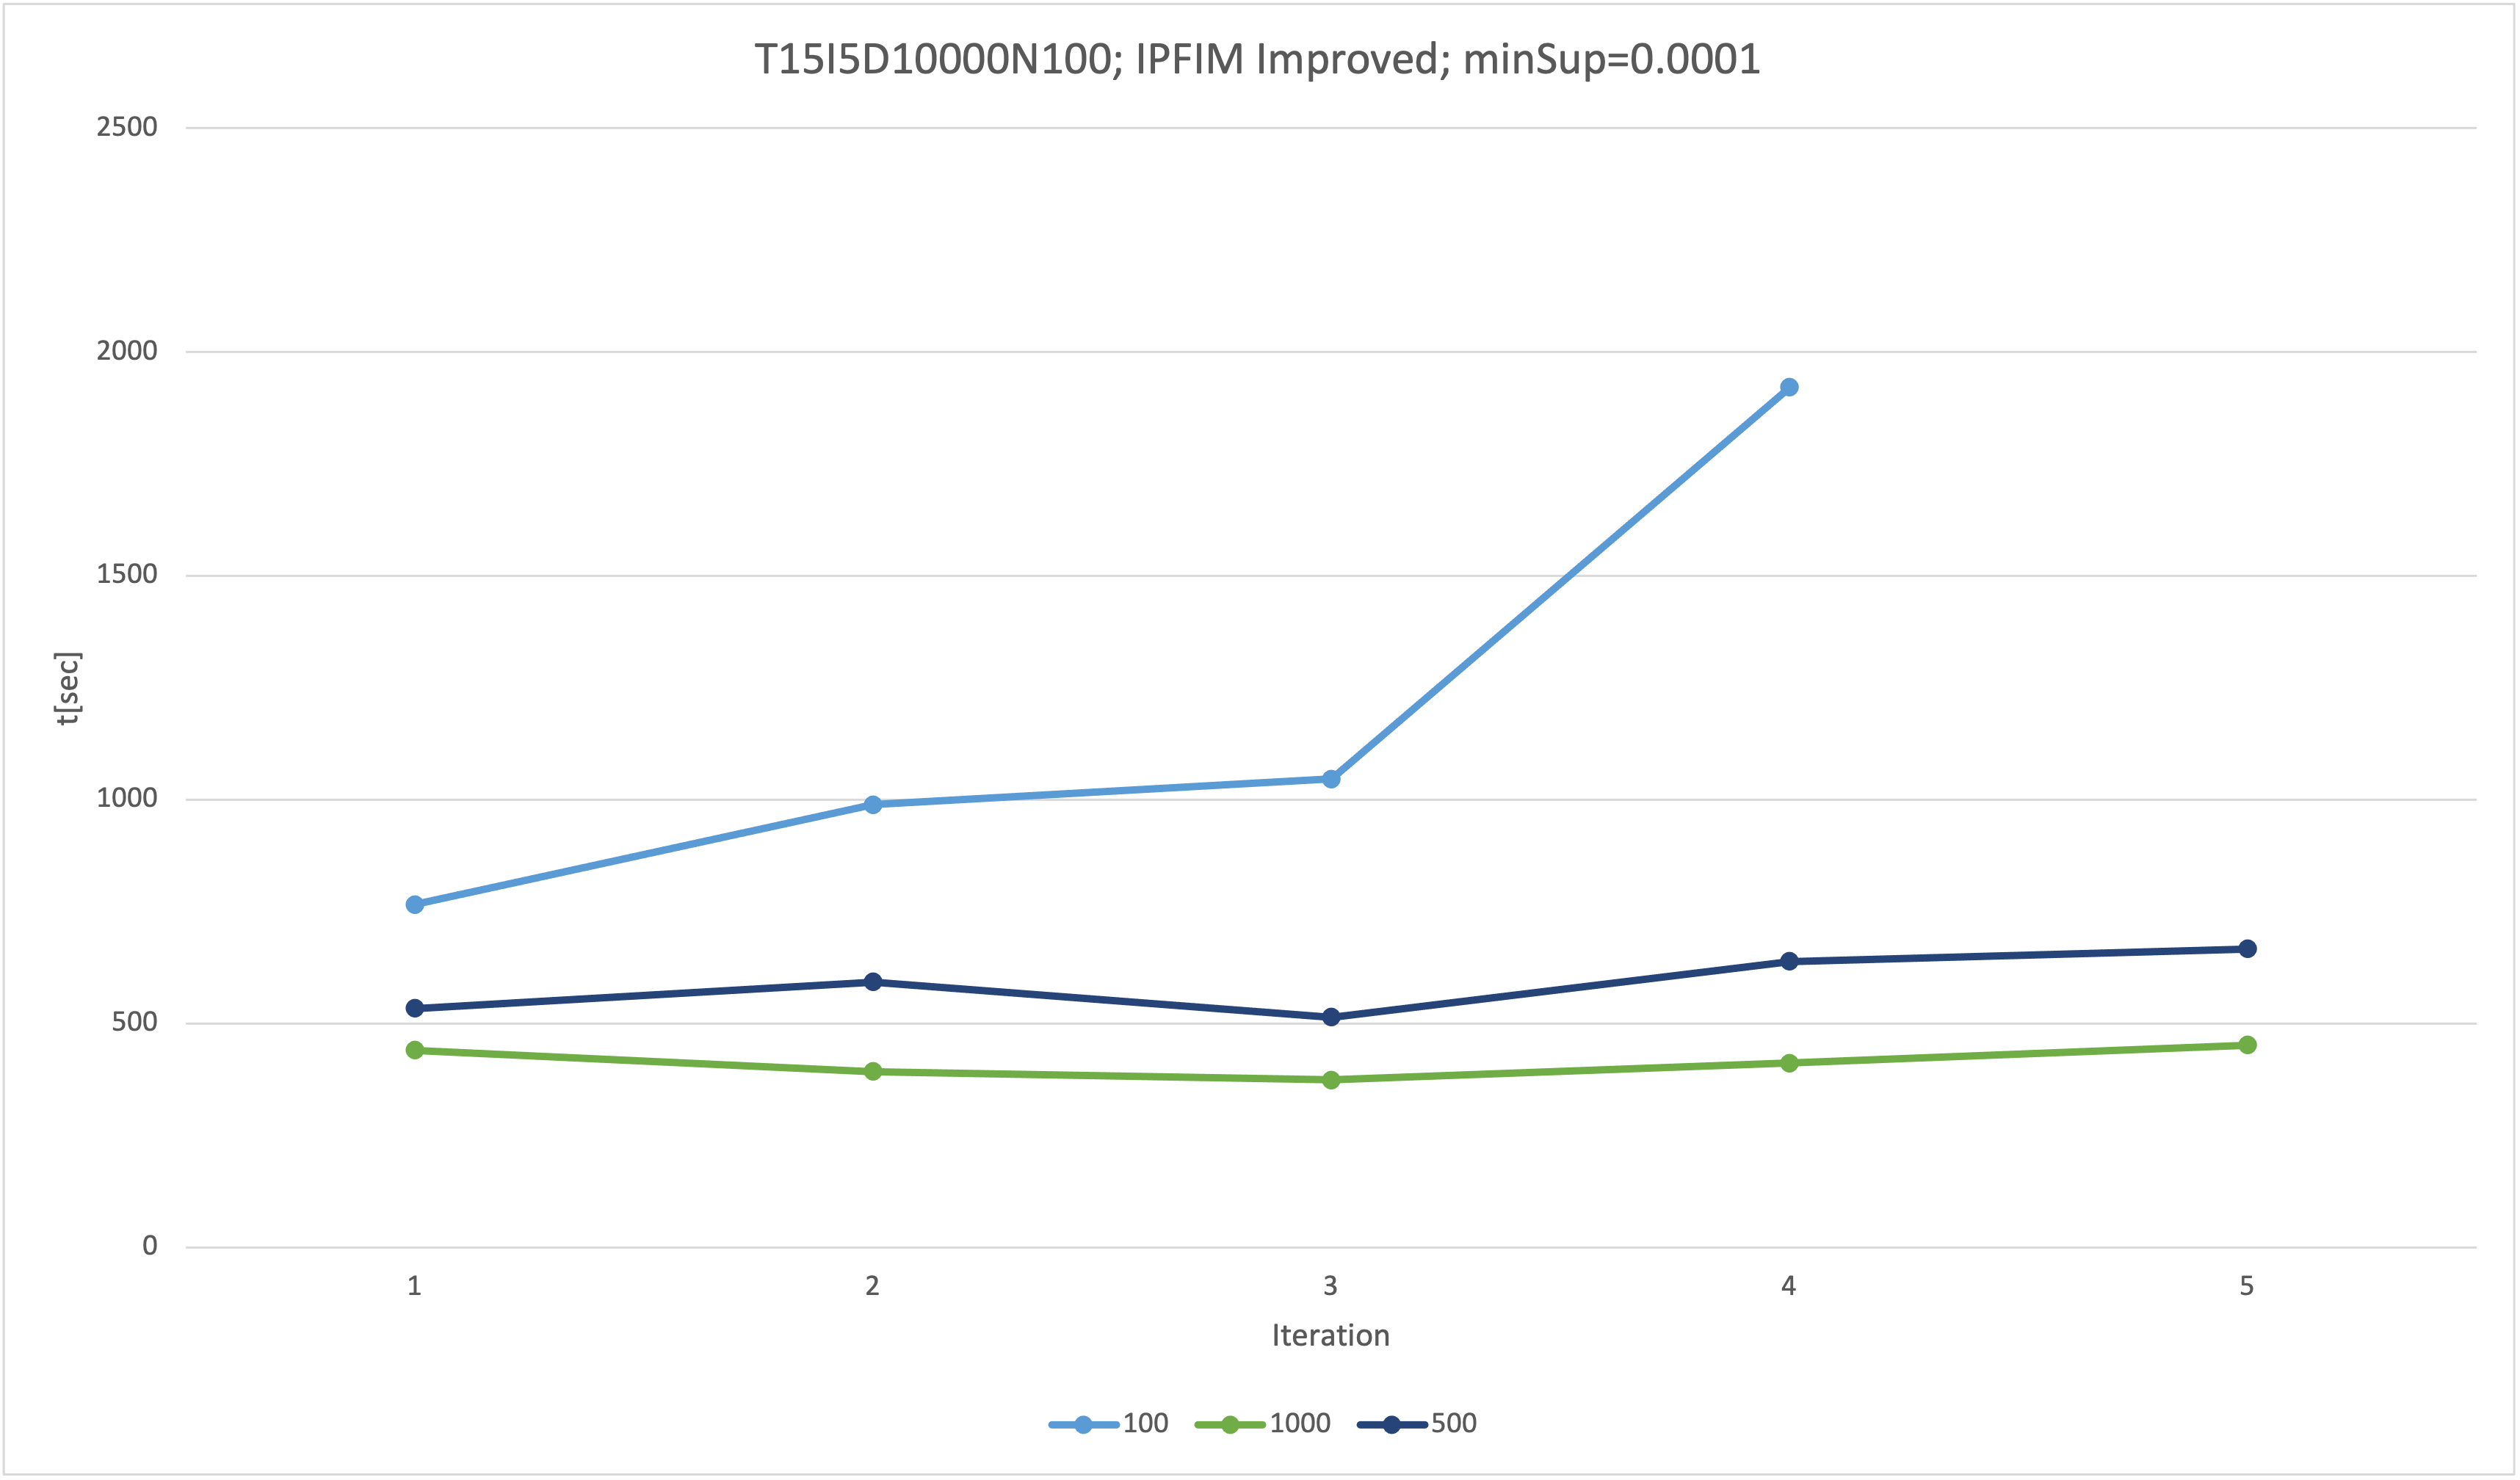
\includegraphics[width=\linewidth]{figures/4iterations/T15I5D10000N100_ipfim_imp_0001}
  \caption{T15I5D10000N100, minSup = 0.0001,  minMinSup = 0.1}
  \label{fig:T15I5D10000N100_ipfim_imp_0001}
    \end{subfigure}  
  \begin{subfigure}{\textwidth}
    \centering
  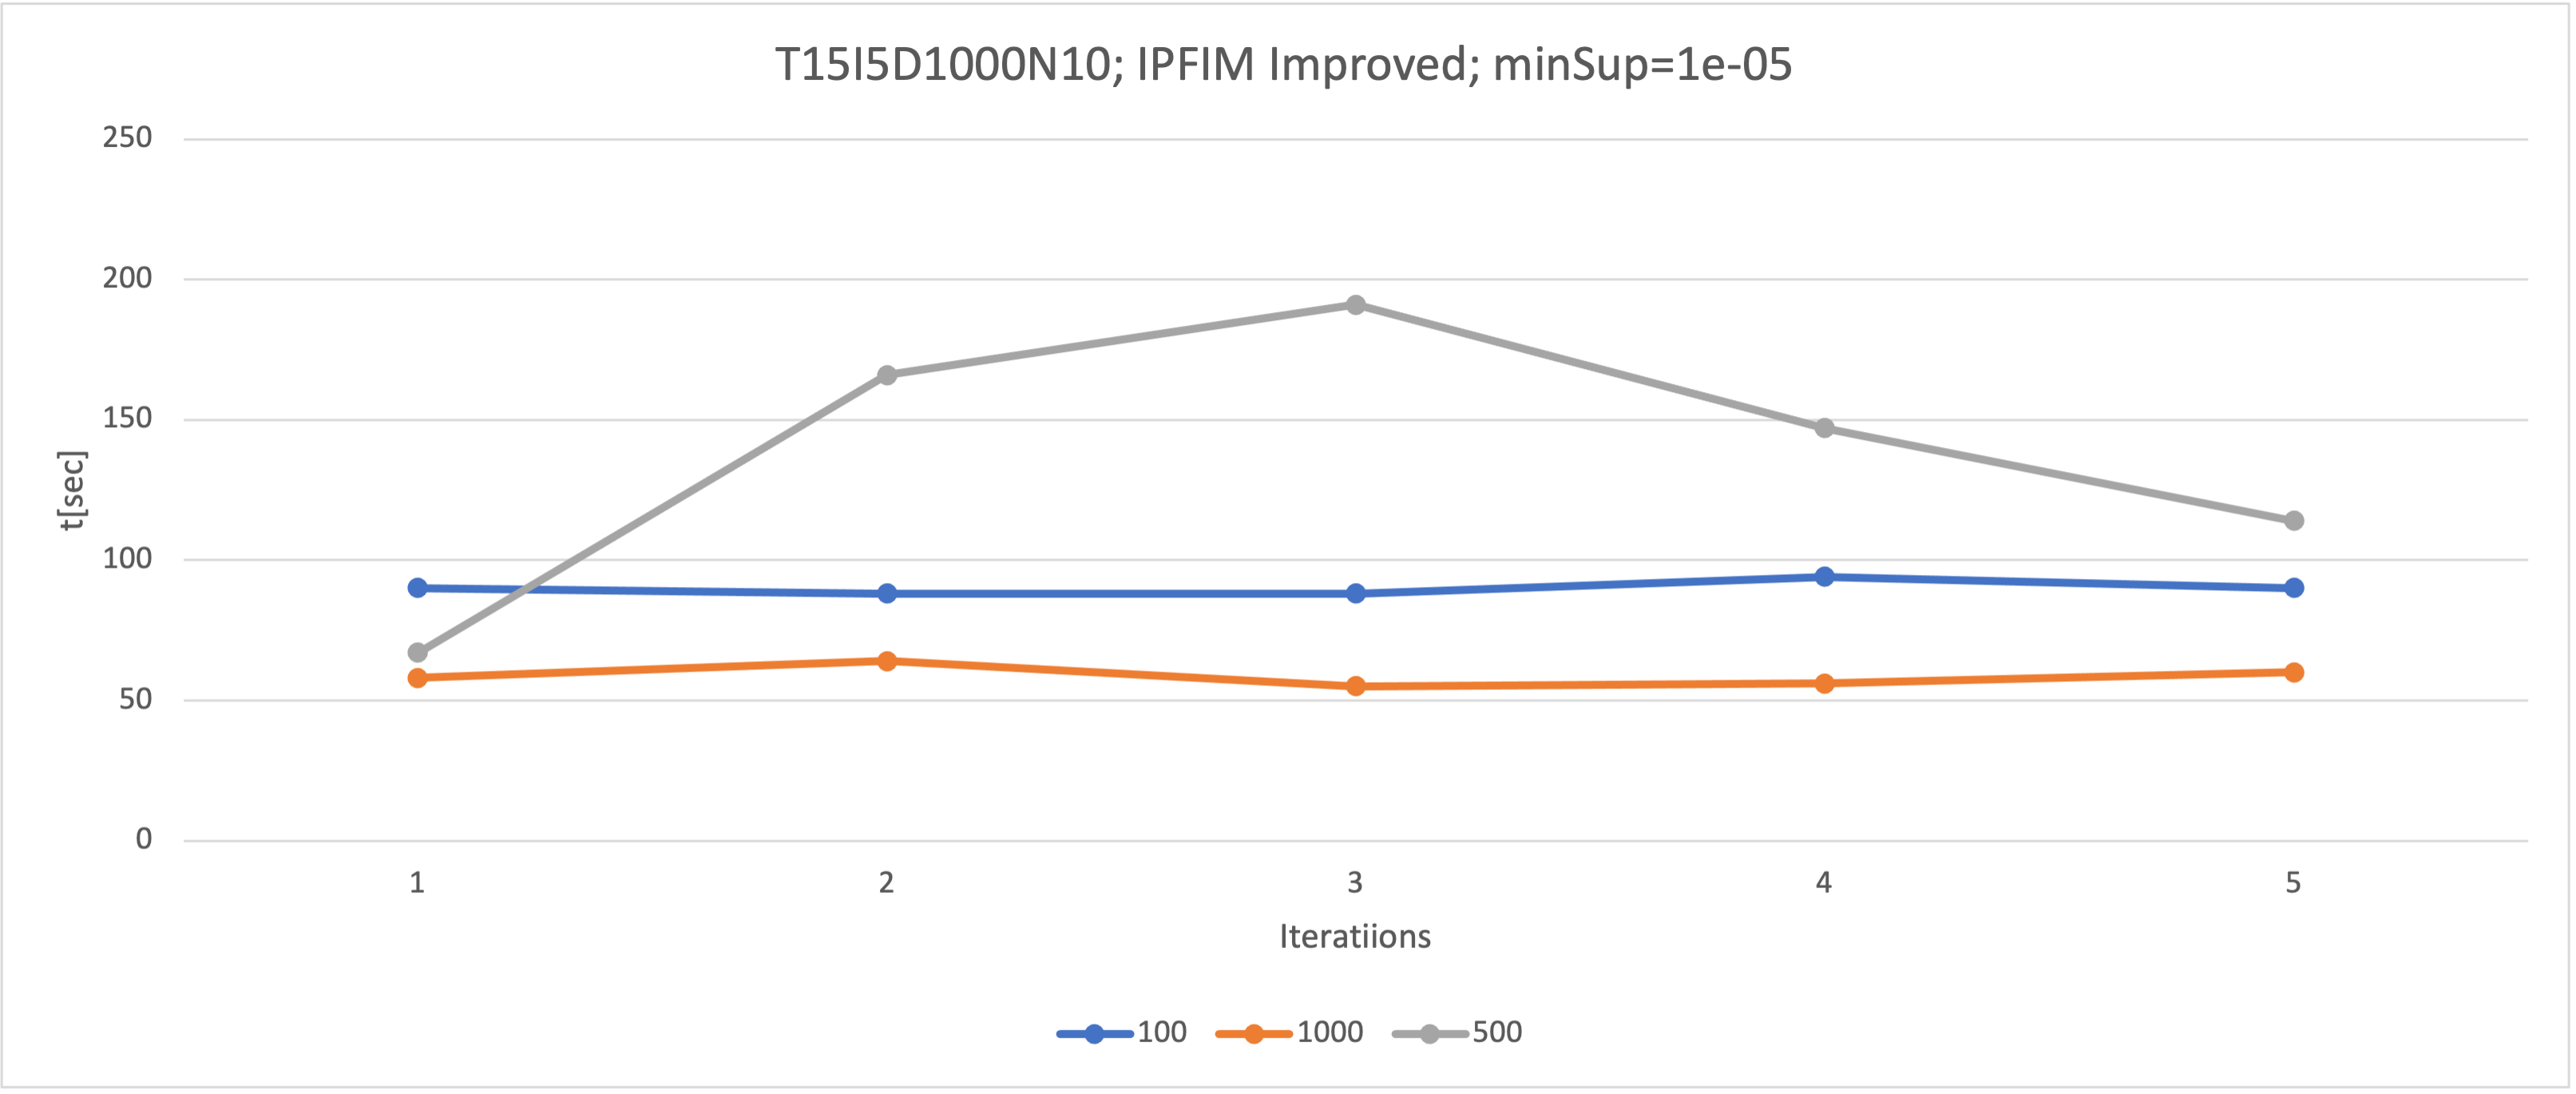
\includegraphics[width=\linewidth]{figures/4iterations/T15I5D1000N10_ipfim_imp_00001}
  \caption{T15I5D1000N10,minSup = 1e-05,  minMinSup = 0.1}
  \label{fig:T15I5D1000N10_ipfim_imp_00001}
    \end{subfigure}  
    \caption{IPFIM Improved 100\textbar 1000\textbar 500 partitions}
\end{figure}



\subsection{Comparing  performance}
To better compare evaluation, we will determine the best partition for a specific data from the results in ~\autoref{sec:resultsstand}, and appropriate minSupport.  ~\autoref{fig:T15I5D1000N10_100_0005} shows that Song has the best performance, while PFP the worst. ~\autoref{fig:kosarak_500part_001} shows best performance for PFP and worse for Song and ~\autoref{fig:T15I5D10000N100_1000part_0001} IPFIM and IPFIM improved has best performance while Song has the worst.

\begin{figure}[H]
  \centering
  \begin{subfigure}{\linewidth}
  \centering
  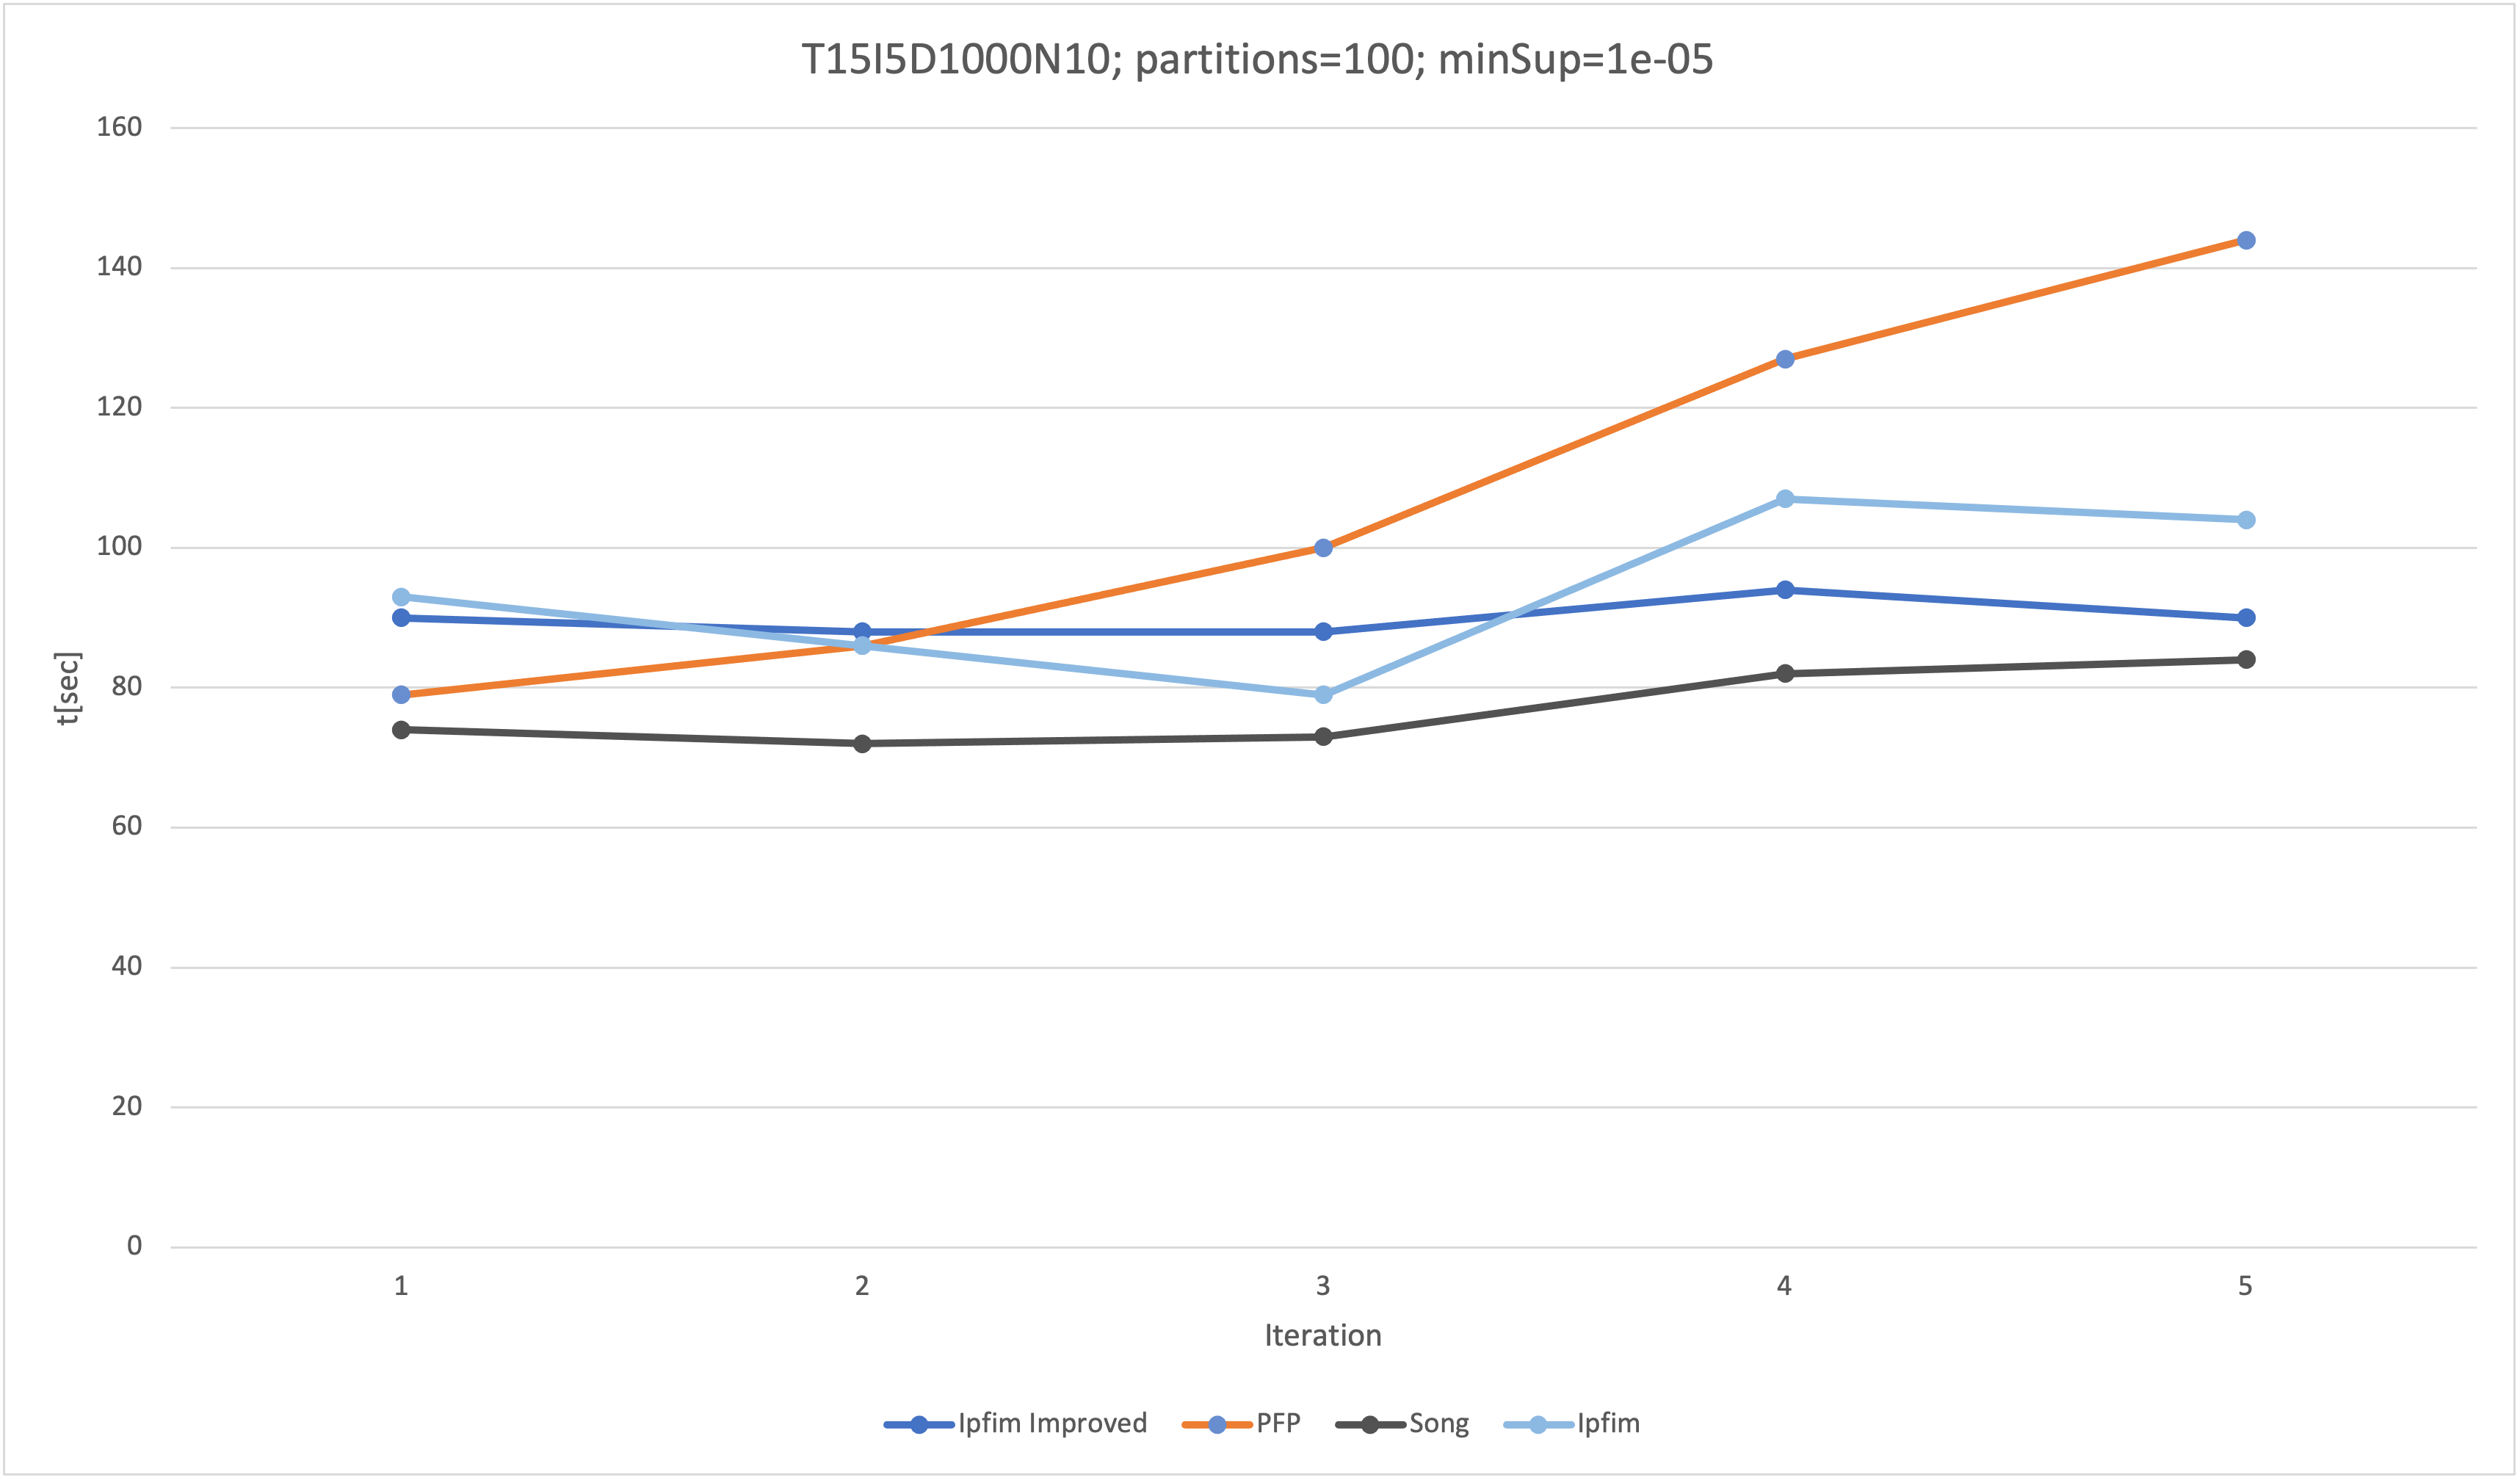
\includegraphics[width=\linewidth, height=\textheight, keepaspectratio]{figures/4iterations/T15I5D1000N10_100_0005}
  \caption{T15I5D1000N10 100 partitions}
  \label{fig:T15I5D1000N10_100_0005}
\end{subfigure}
  \begin{subfigure}{\linewidth}
  \centering
  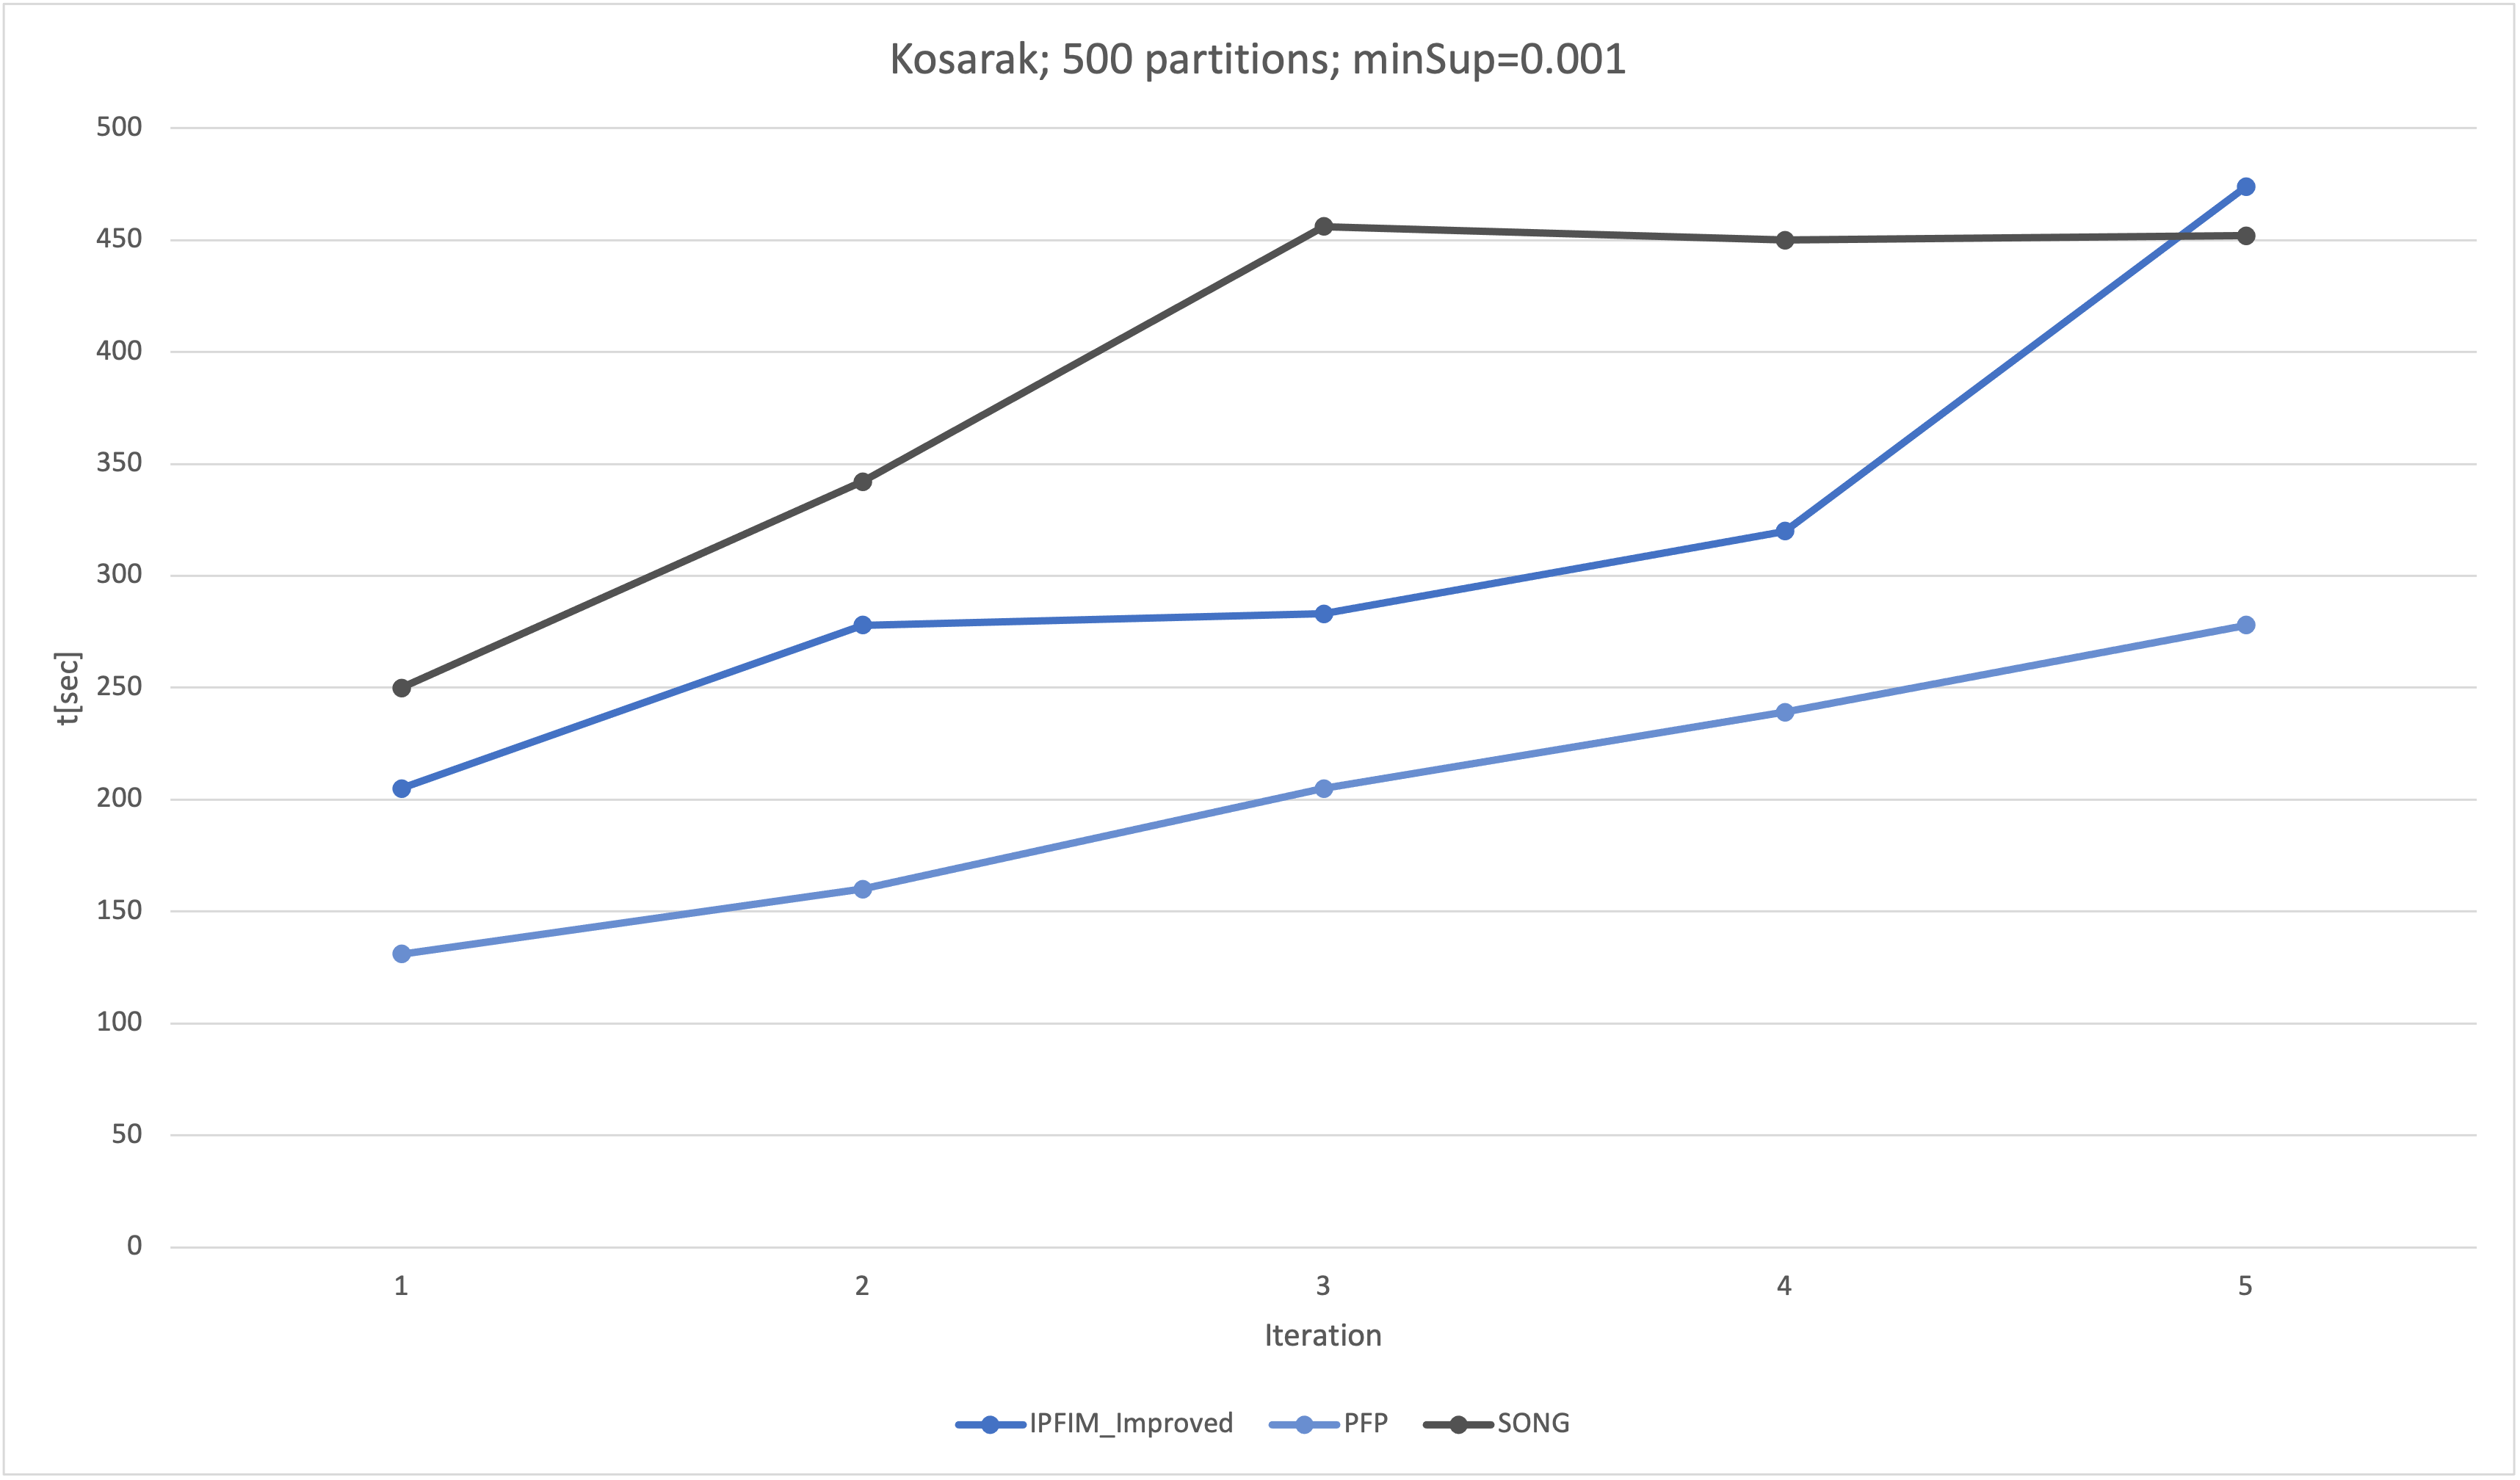
\includegraphics[width=\linewidth ,height=\textheight, keepaspectratio]{figures/4iterations/kosarak_500part_001}
  \caption{kosarak, minSup = 0.001,  partitions = 500}
  \label{fig:kosarak_500part_001}
\end{subfigure}
  \begin{subfigure}{\linewidth}
  \centering
  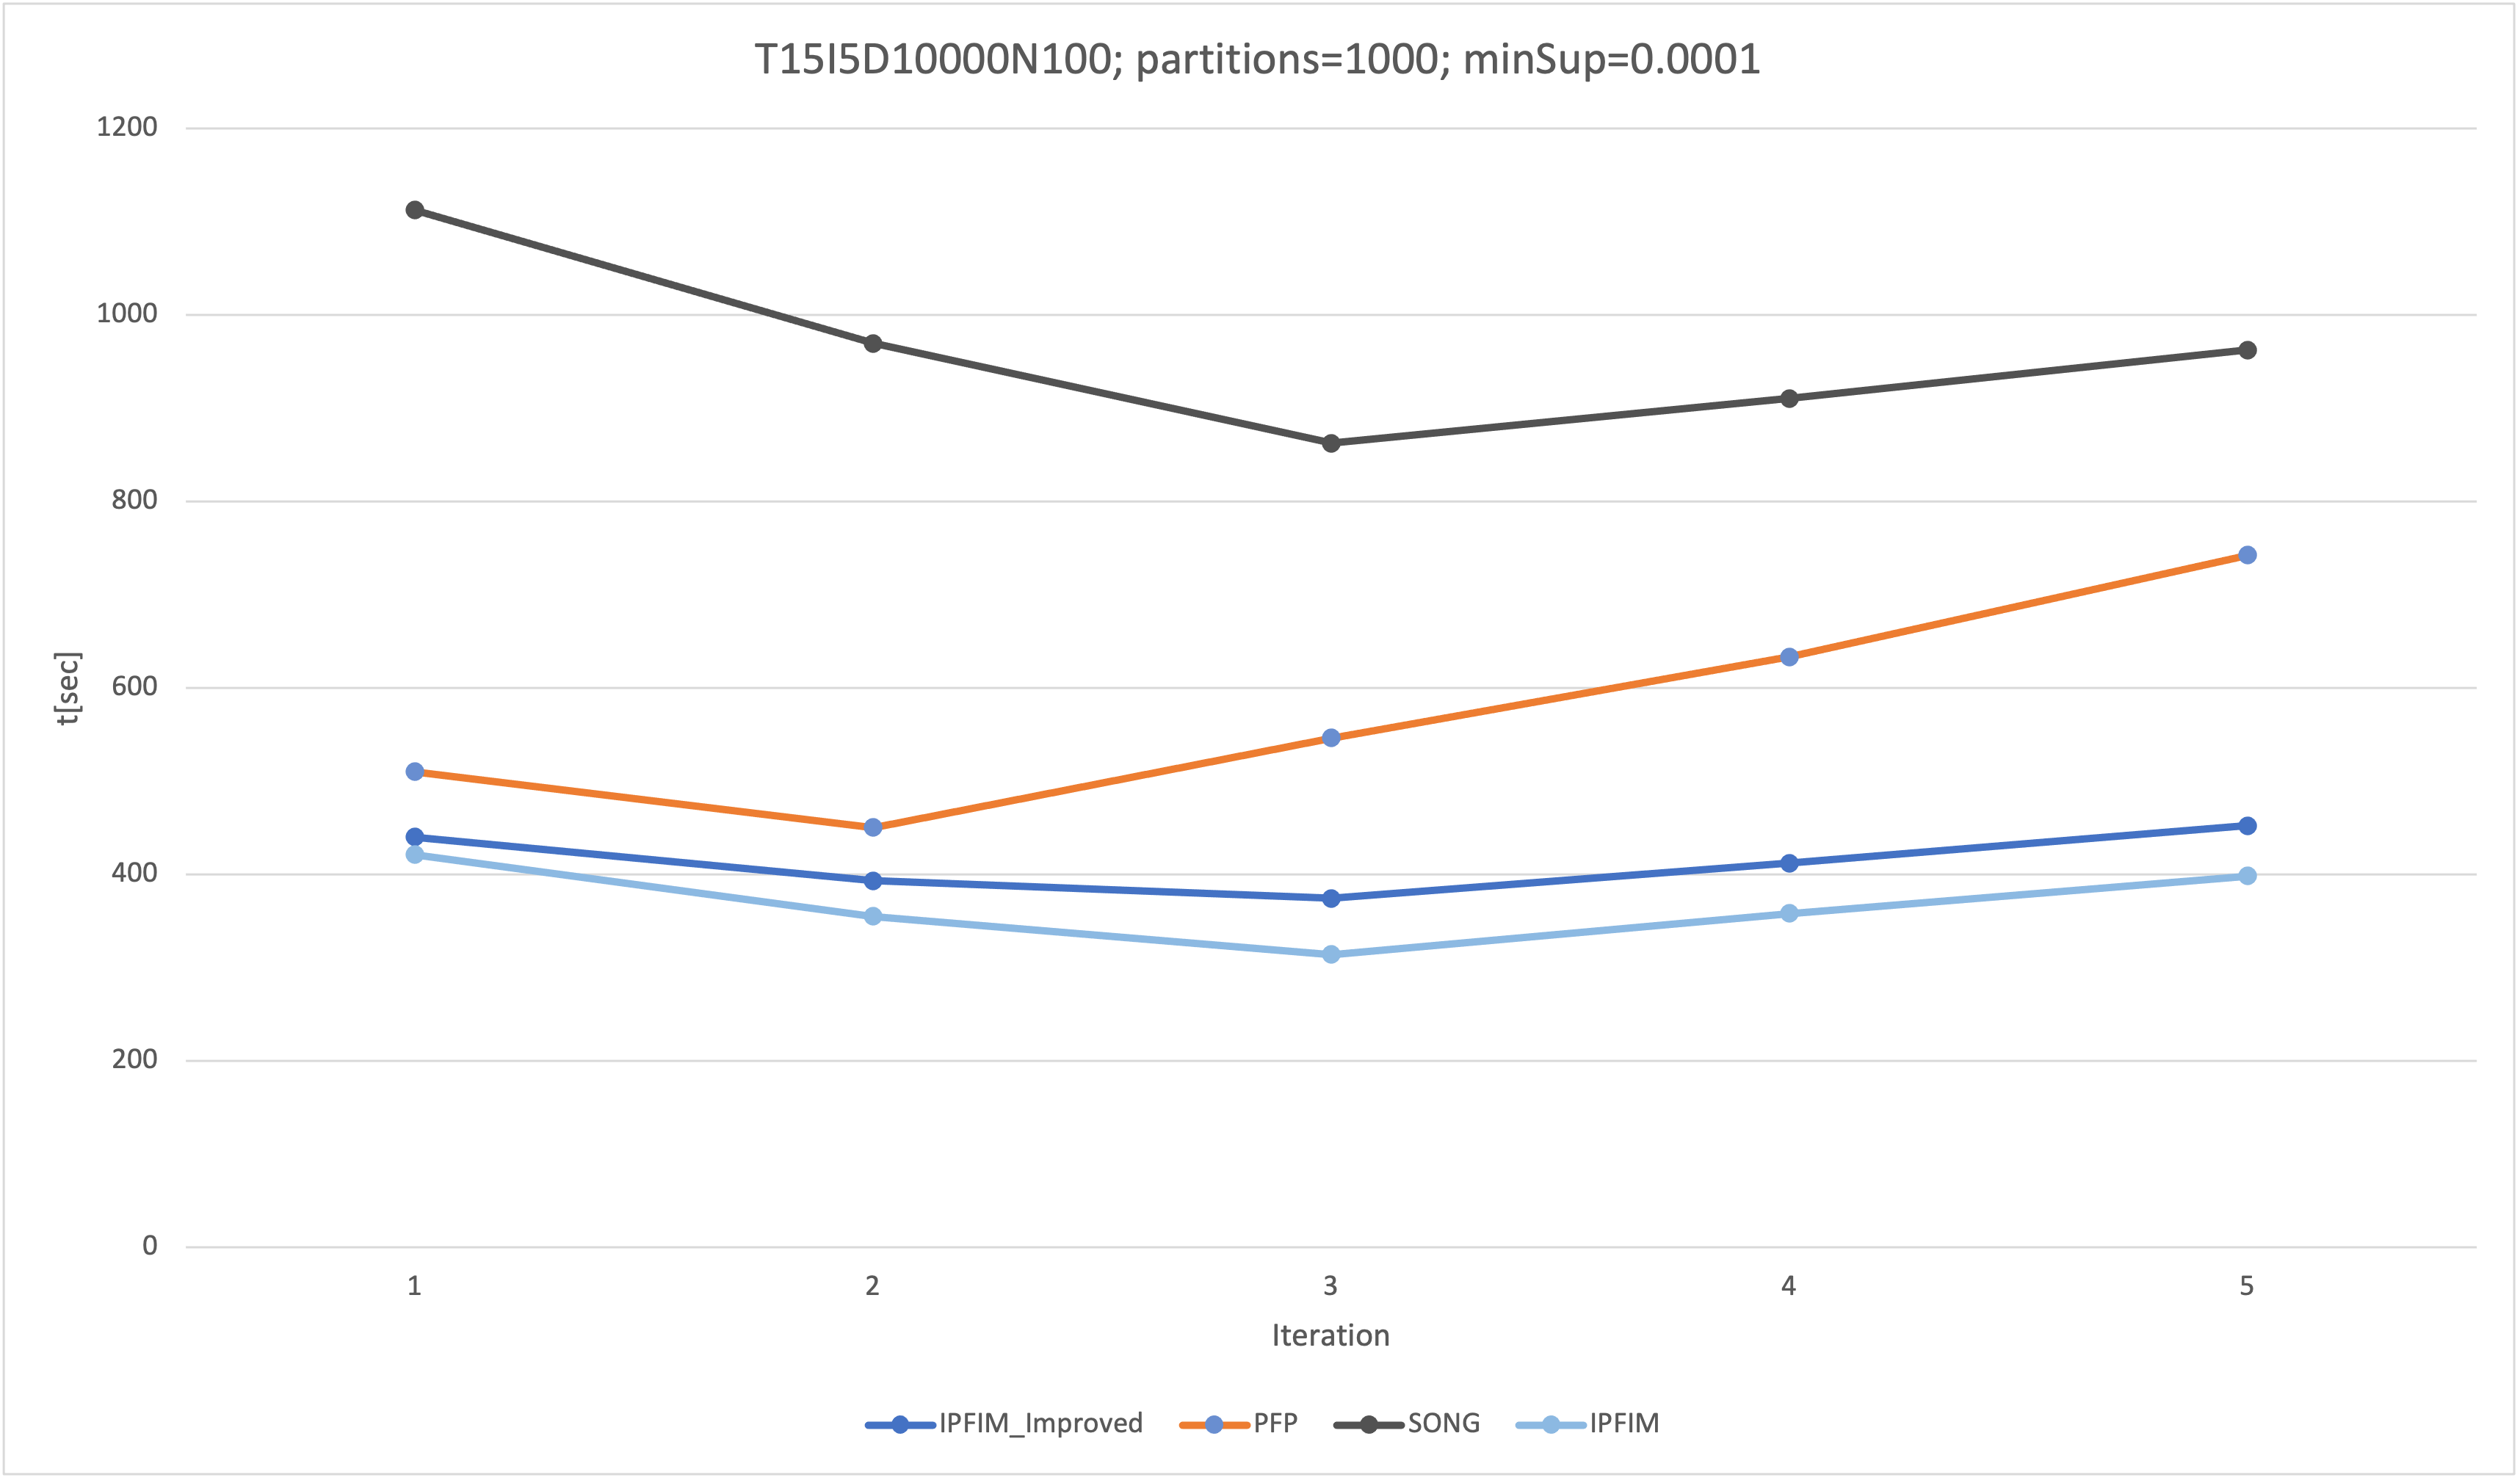
\includegraphics[width=\linewidth ,height=\textheight, keepaspectratio]{figures/4iterations/T15I5D10000N100_1000part_0001}
  \caption{T15I5D10000N100, minSup = 0.0001,  1000 partitions}
  \label{fig:T15I5D10000N100_1000part_0001}
\end{subfigure}
\caption{Comparison of the different algorithms}
\end{figure}

For the Set-Cover algorithm, ~\autoref{fig:T15I5D10000N100_1000part_SETCOVER_0001} shows that the reshuffleing of the partitions using map hash is extremely slow compared to a rand hash function, used in the original algorithm.
\begin{figure}[H]
  \centering
  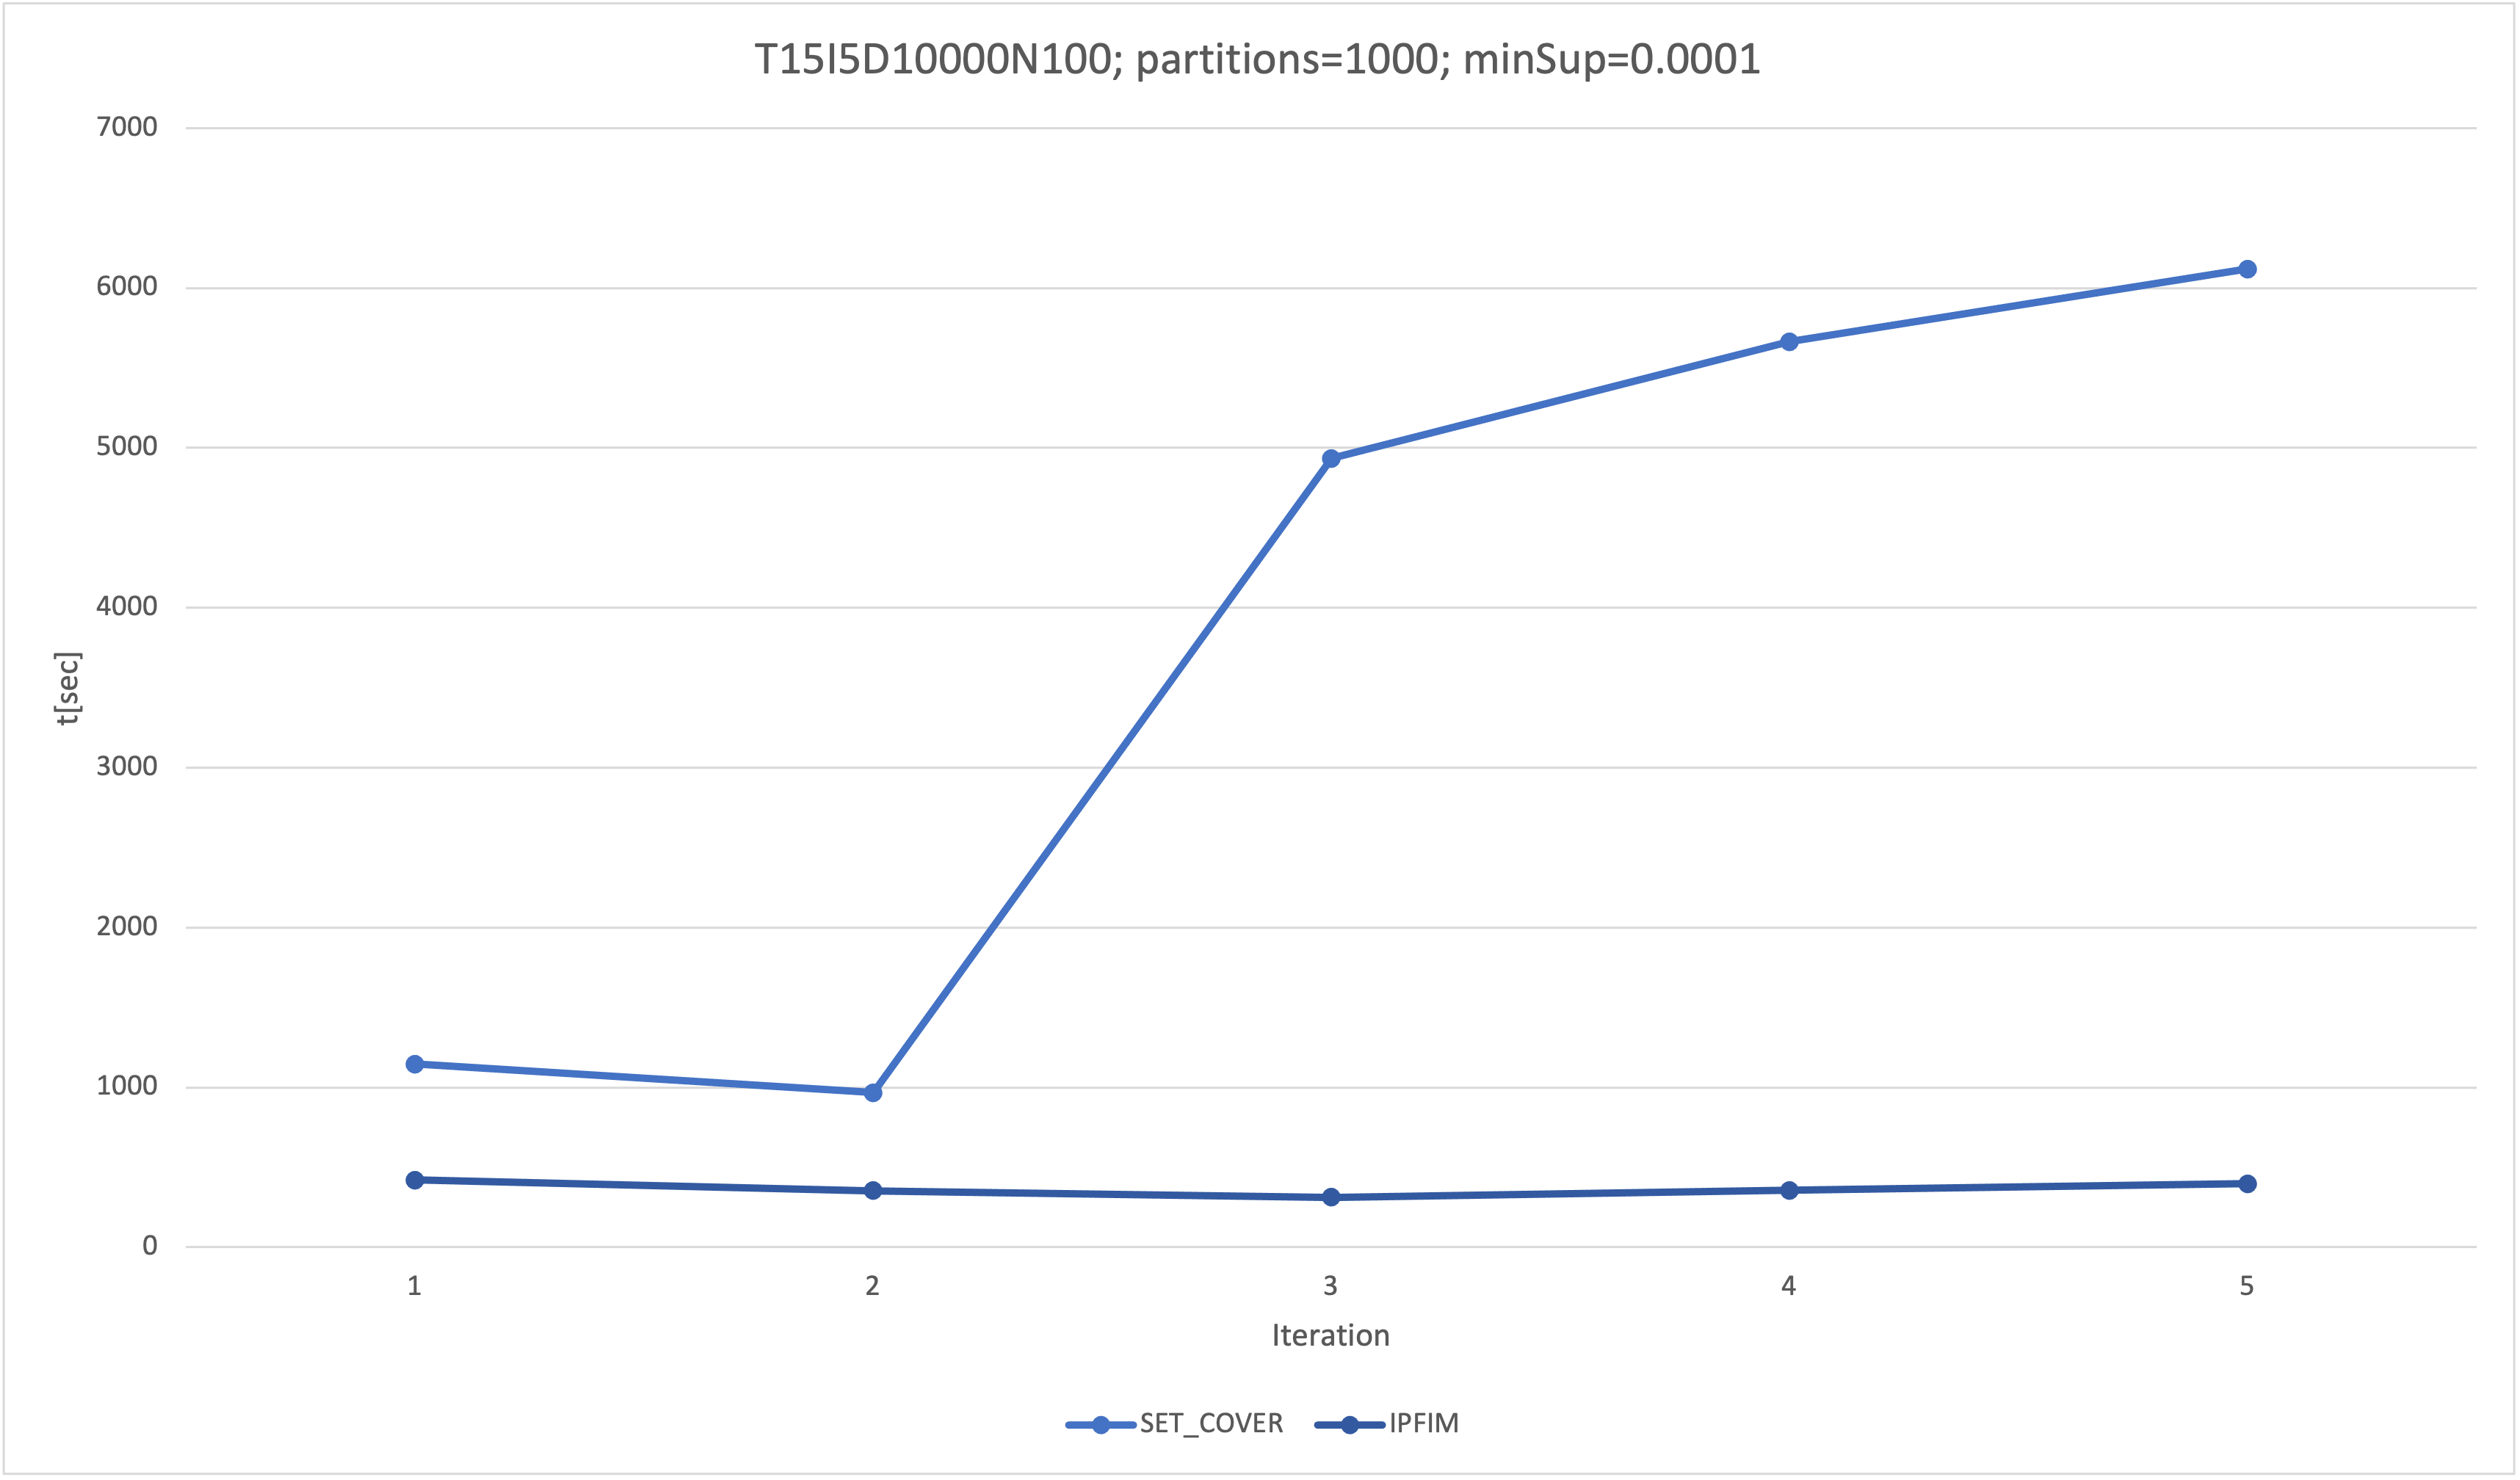
\includegraphics[width=\linewidth]{figures/4iterations/T15I5D10000N100_1000part_SETCOVER_0001}
  \caption{T15I5D10000N100, minSup = 0.0001,  1000 partitions, Set cover vs IPFIM}
  \label{fig:T15I5D10000N100_1000part_SETCOVER_0001}
\end{figure}


\subsection{Tree size evaluation - Standalone}
For the tree size evaluation, we collected the statistics of maximum, average and minimum tree size in each iteration. 

\paragraph{PFP} For ~\autoref{fig:T15I5D10000N100_MaxTree_PFP_0001} the ratio is 0.21 and 0.116 between the different partitions, however for ~\autoref{fig:T15I5D10000N100_AvgTree_PFP_0001} it is the partitions ration - 0.20 and 0.1 (similar to partitions ratio) .

\begin{figure}[H]
  \centering
  \begin{subfigure}{\linewidth}
  \centering
  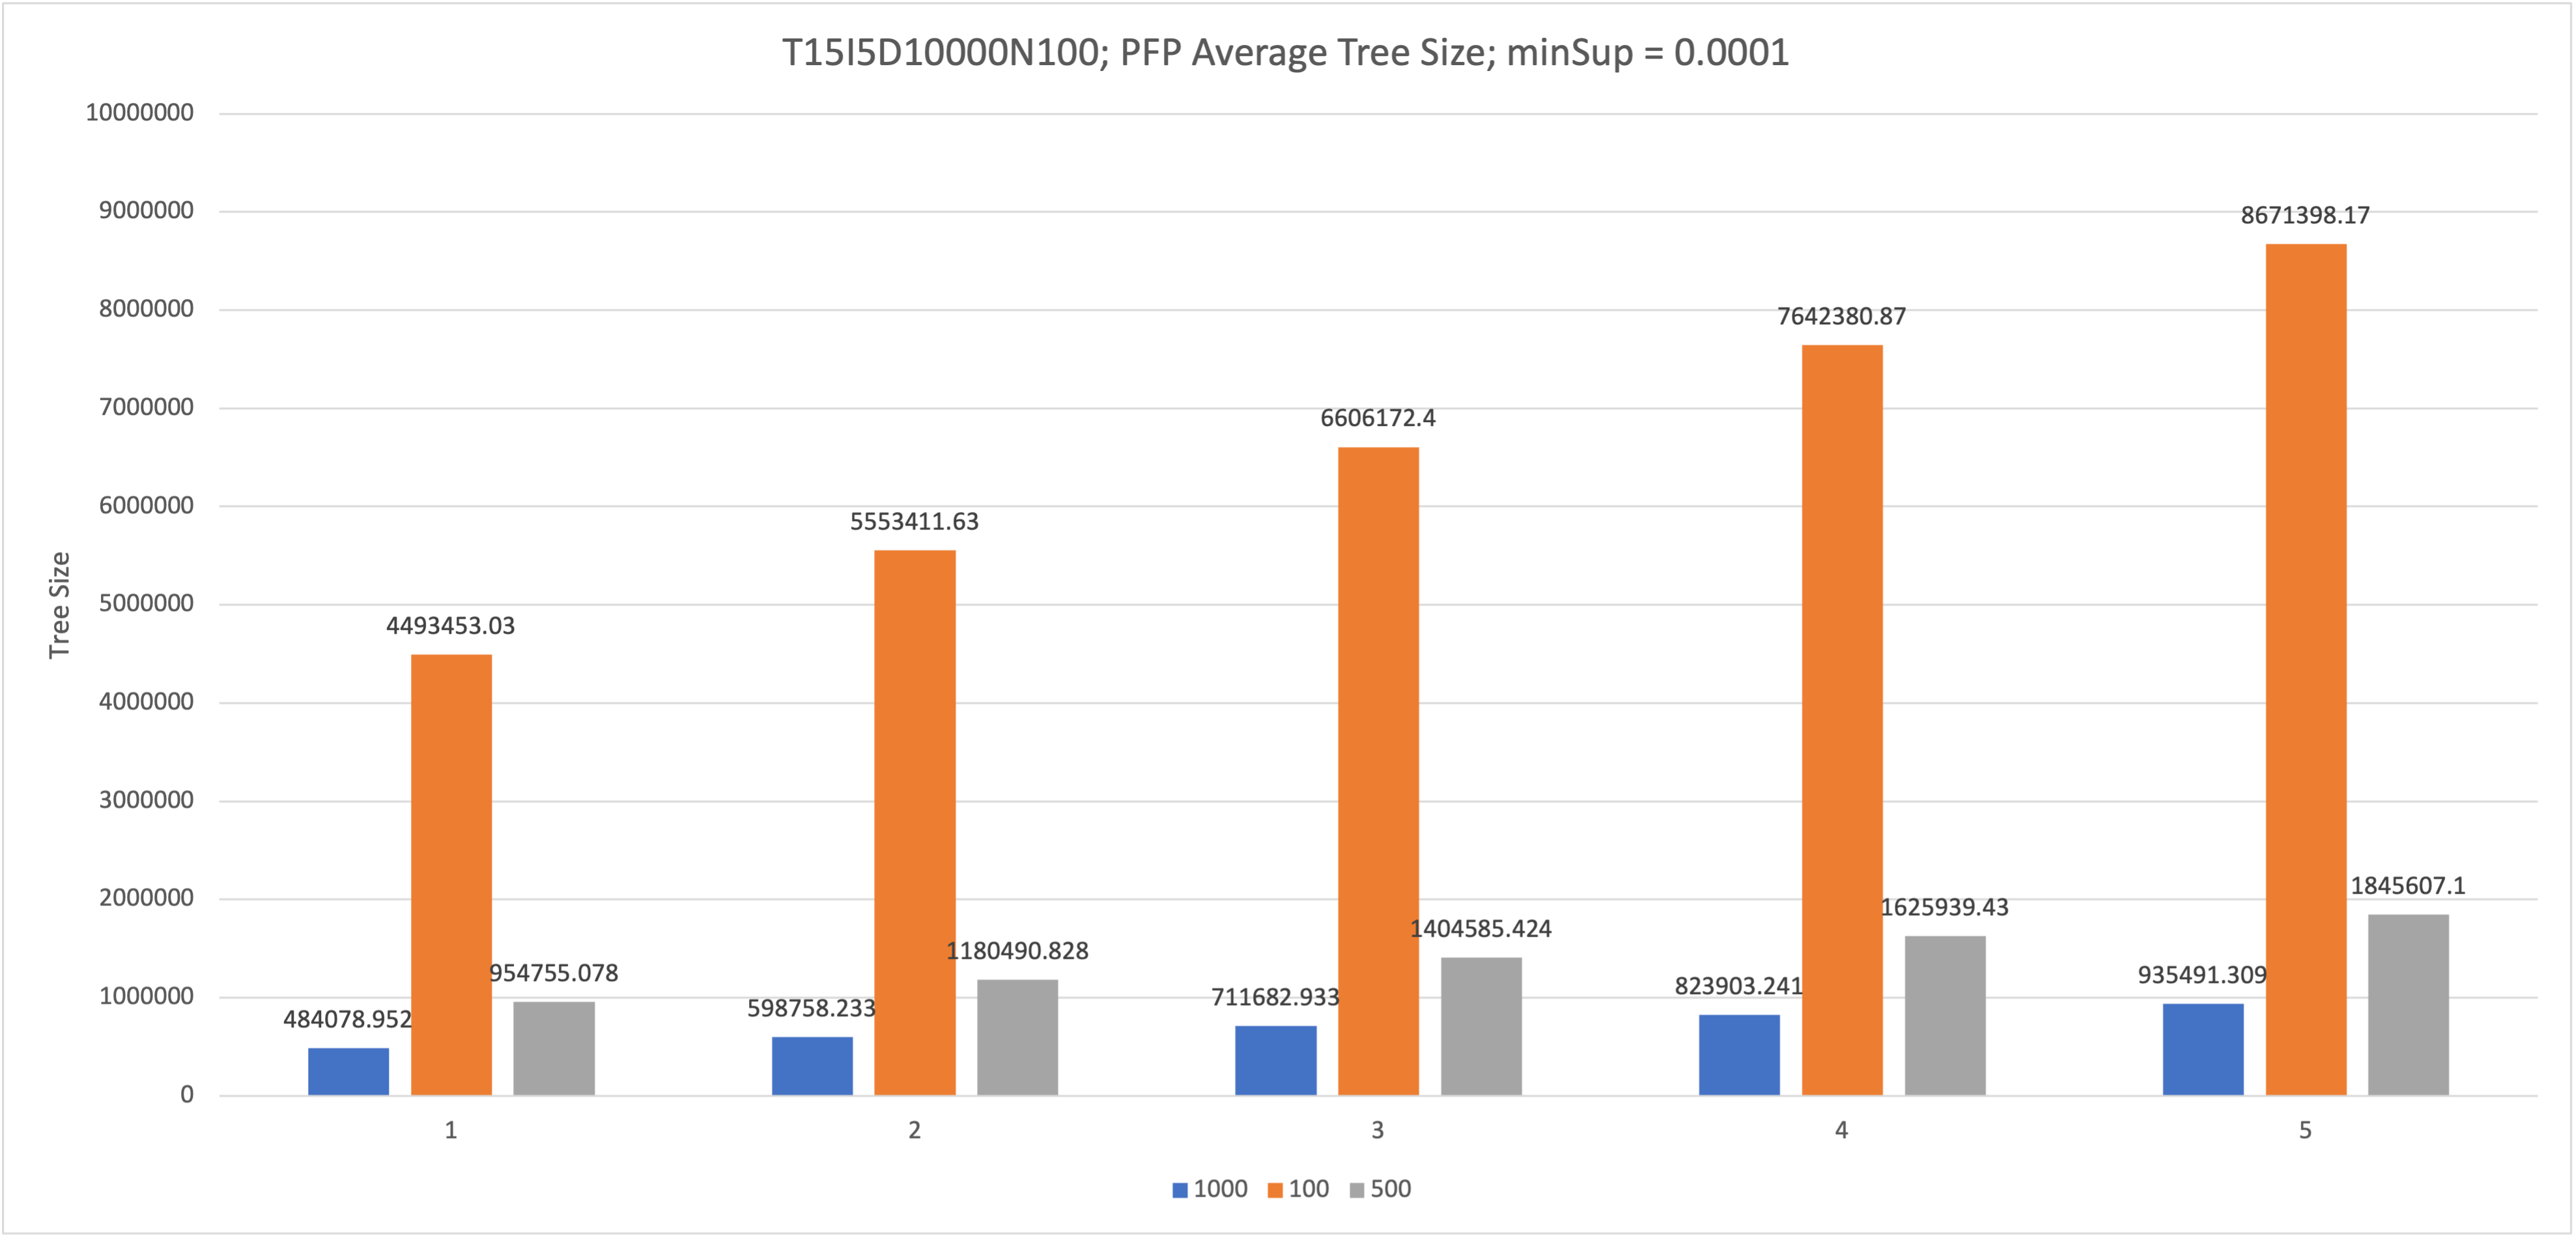
\includegraphics[width=\linewidth ,height=\textheight, keepaspectratio]{figures/4iterations/T15I5D10000N100_AvgTree_PFP_0001}
  \caption{T15I5D10000N100 PFP Average tree size}
  \label{fig:T15I5D10000N100_AvgTree_PFP_0001}
\end{subfigure}
  \begin{subfigure}{\linewidth}
  \centering
  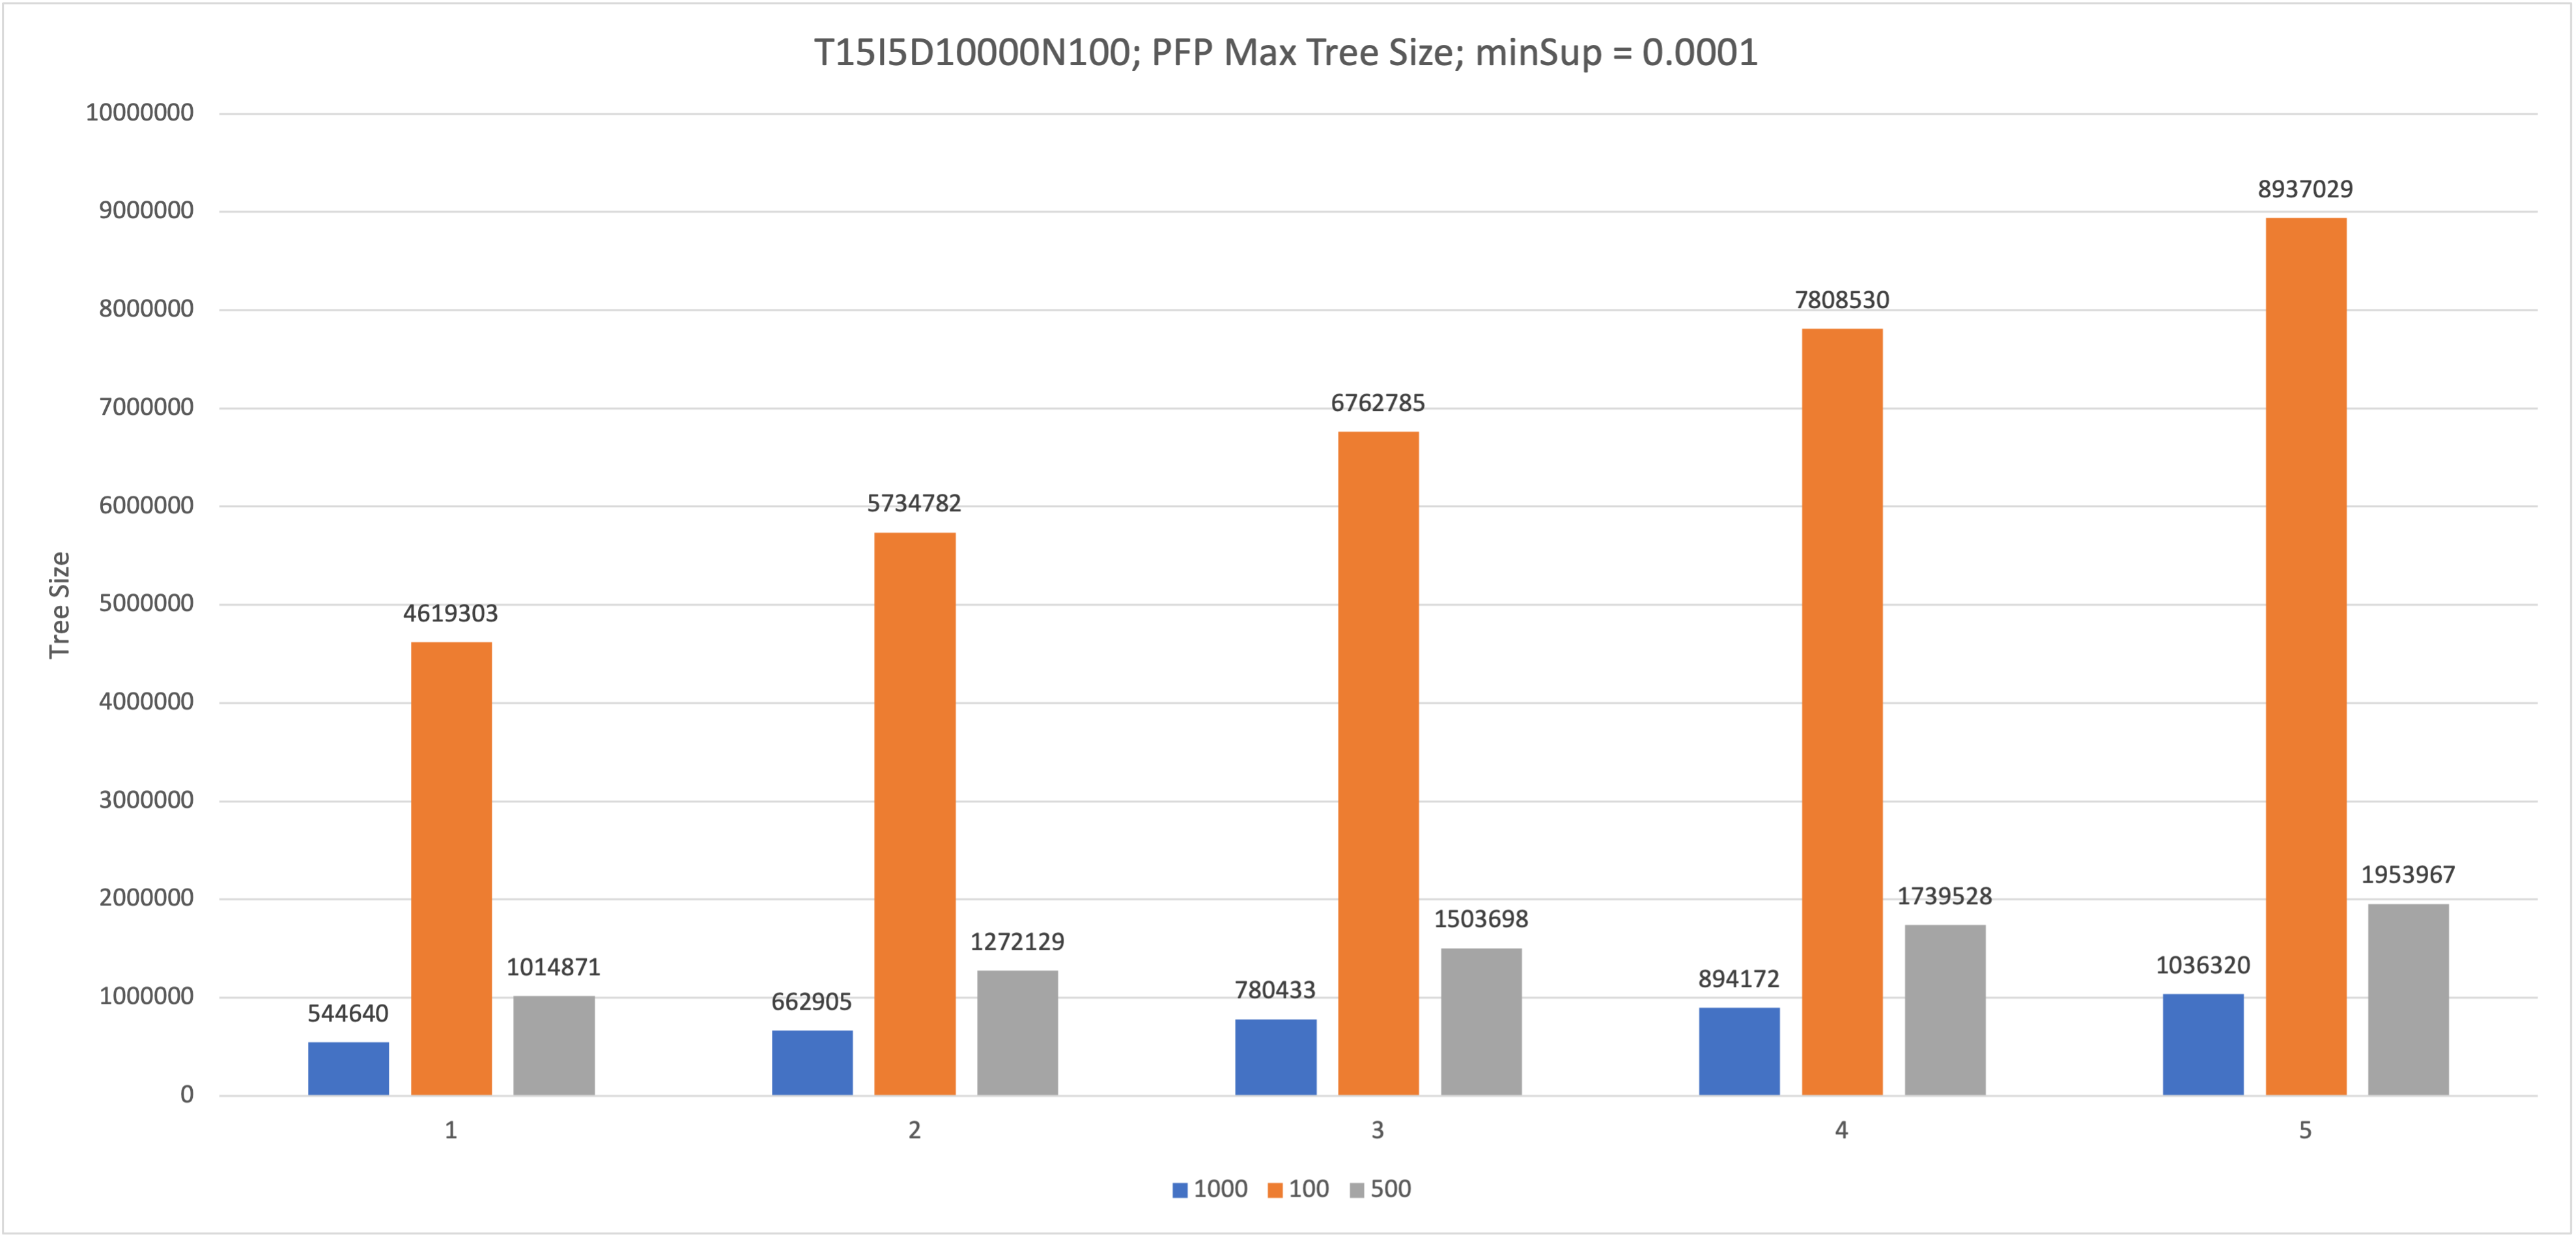
\includegraphics[width=\linewidth ,height=\textheight, keepaspectratio]{figures/4iterations/T15I5D10000N100_MaxTree_PFP_0001}
  \caption{T15I5D10000N100 PFP Max tree size}
  \label{fig:T15I5D10000N100_MaxTree_PFP_0001}
\end{subfigure}
\caption{T15I5D10000N100 PFP Average and Max tree size for 100\textbar 1000\textbar 500 partitions}
\end{figure}

\paragraph{Song}
For ~\autoref{fig:T15I5D10000N100_MaxTree_Song_0001} the ratio is 0.3 and 0.17 between the different partitions, however for ~\autoref{fig:T15I5D10000N100_AvgTree_Song_0001} it is the partitions ration - 0.2 and 0.1 (same as partitions ratio).

\begin{figure}[H]
  \centering
  \begin{subfigure}{\linewidth}
  \centering
  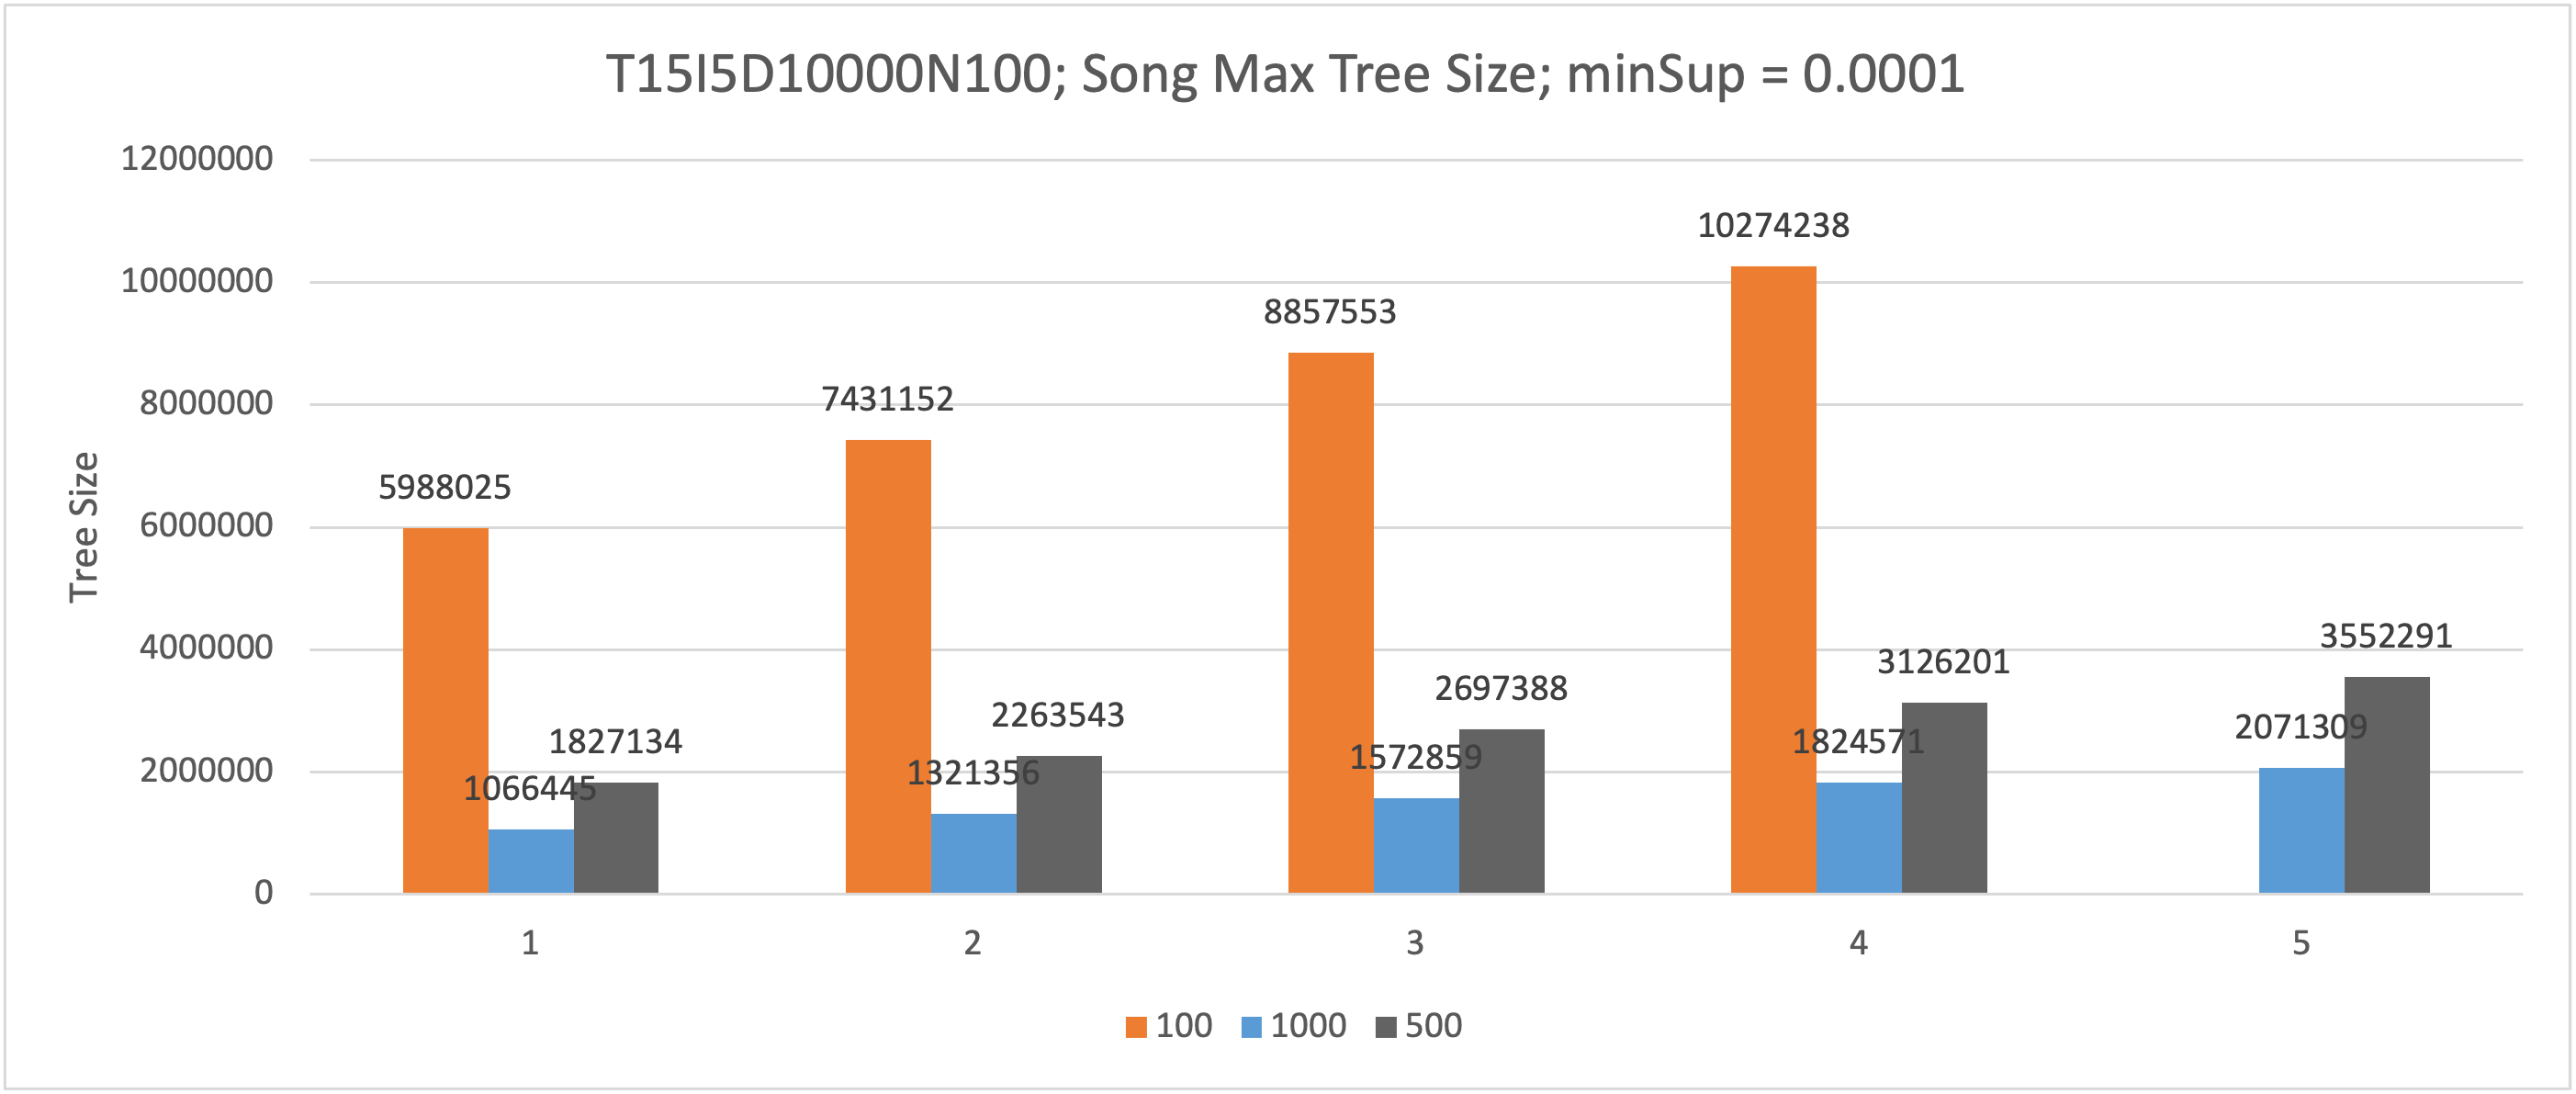
\includegraphics[width=\linewidth ,height=\textheight, keepaspectratio]{figures/4iterations/T15I5D10000N100_MaxTree_Song_0001}
  \caption{T15I5D10000N100 Song Max tree size}
  \label{fig:T15I5D10000N100_MaxTree_Song_0001}
\end{subfigure}
  \begin{subfigure}{\linewidth}
  \centering
  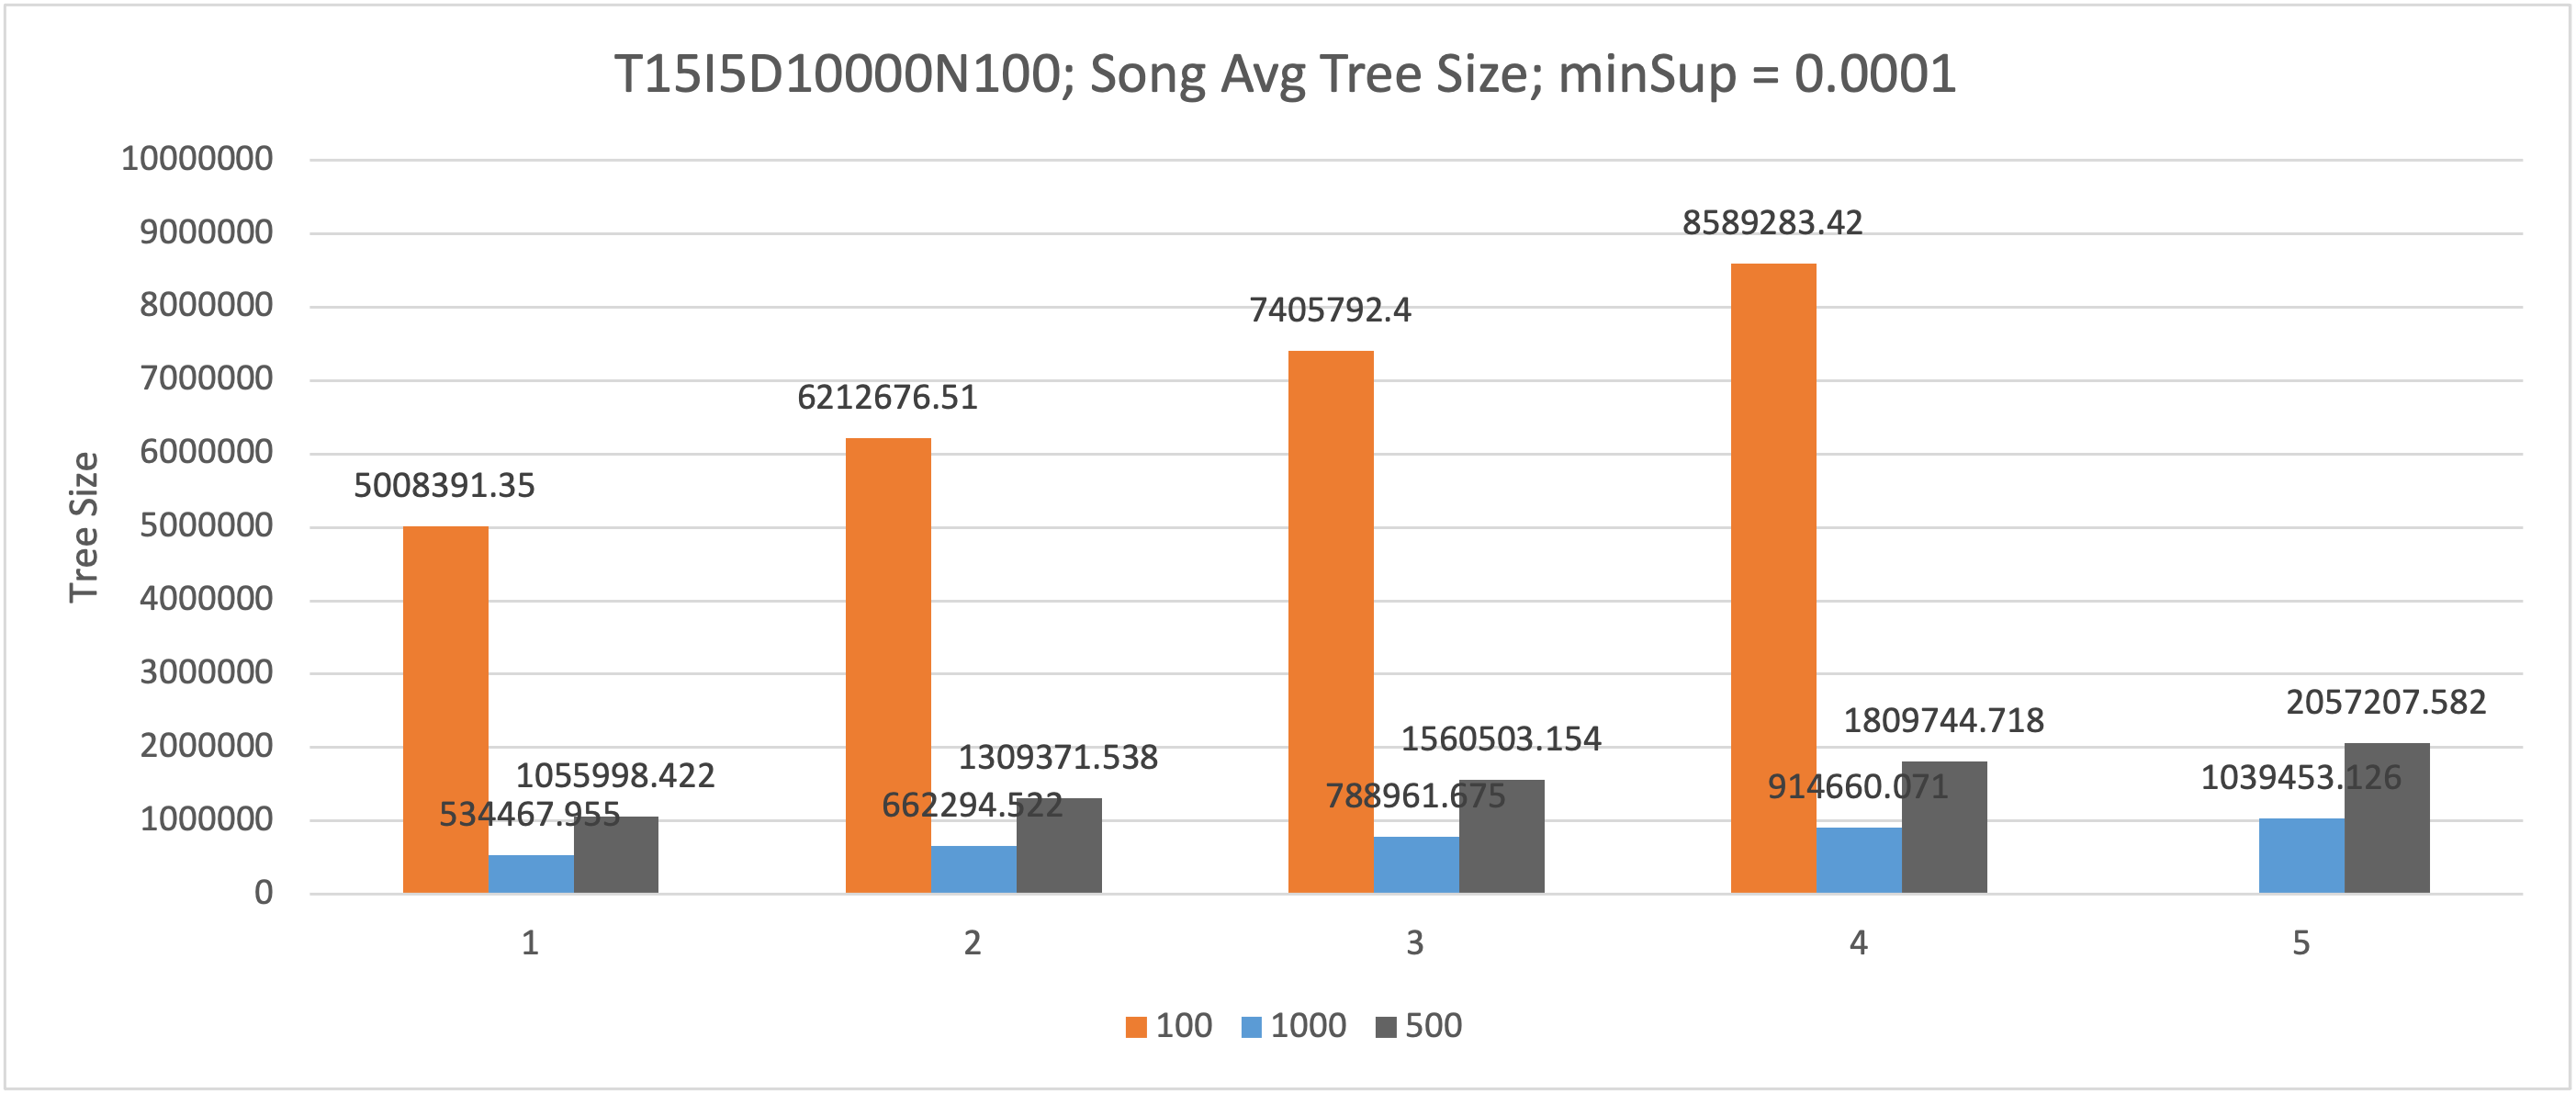
\includegraphics[width=\linewidth ,height=\textheight, keepaspectratio]{figures/4iterations/T15I5D10000N100_AvgTree_Song_0001}
  \caption{T15I5D10000N100 Song Average tree size}
  \label{fig:T15I5D10000N100_AvgTree_Song_0001}
\end{subfigure}
\caption{T15I5D10000N100 Song Average and Max tree size for 100\textbar 1000\textbar 500 partitions}
\end{figure}

\paragraph{IPFIM}
For ~\autoref{fig:T15I5D10000N100_MaxTree_IPFIM_0001} the ratio is 0.3 and 0.177 between the different partitions, however for ~\autoref{fig:T15I5D10000N100_AvgTree_IPFIM_0001} it is the partitions ration - 0.2 and 0.1 (same as partitions ratio).

\begin{figure}
  \centering
  \begin{subfigure}{\linewidth}
  \centering
  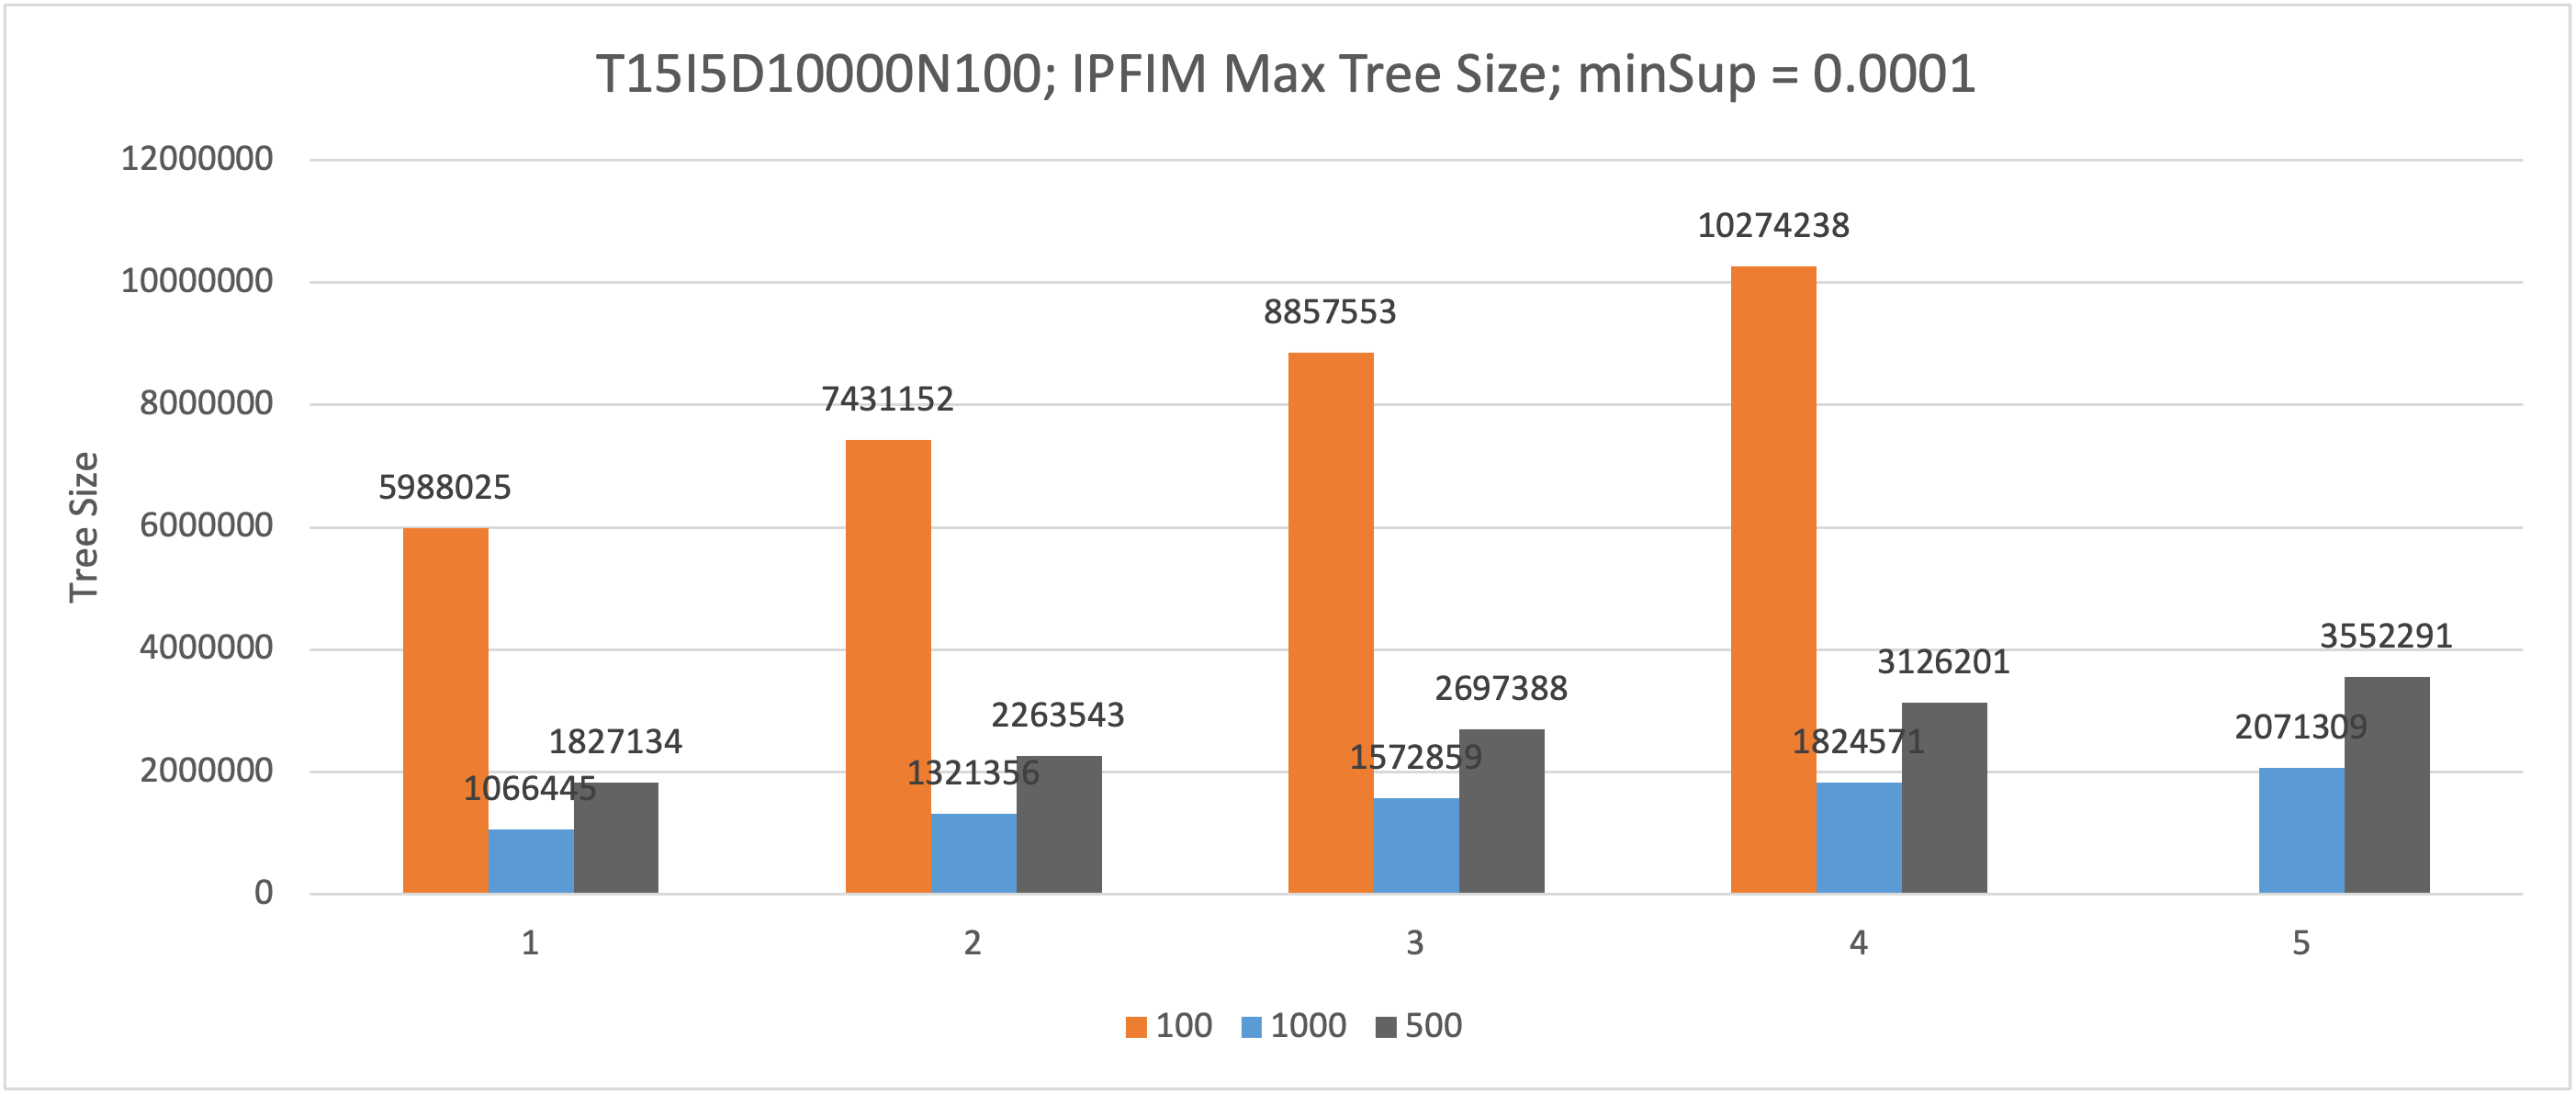
\includegraphics[width=\linewidth ,height=\textheight, keepaspectratio]{figures/4iterations/T15I5D10000N100_MaxTree_IPFIM_0001}
  \caption{T15I5D10000N100 IPFIM Max tree size}
  \label{fig:T15I5D10000N100_MaxTree_IPFIM_0001}
\end{subfigure}
  \begin{subfigure}{\linewidth}
  \centering
  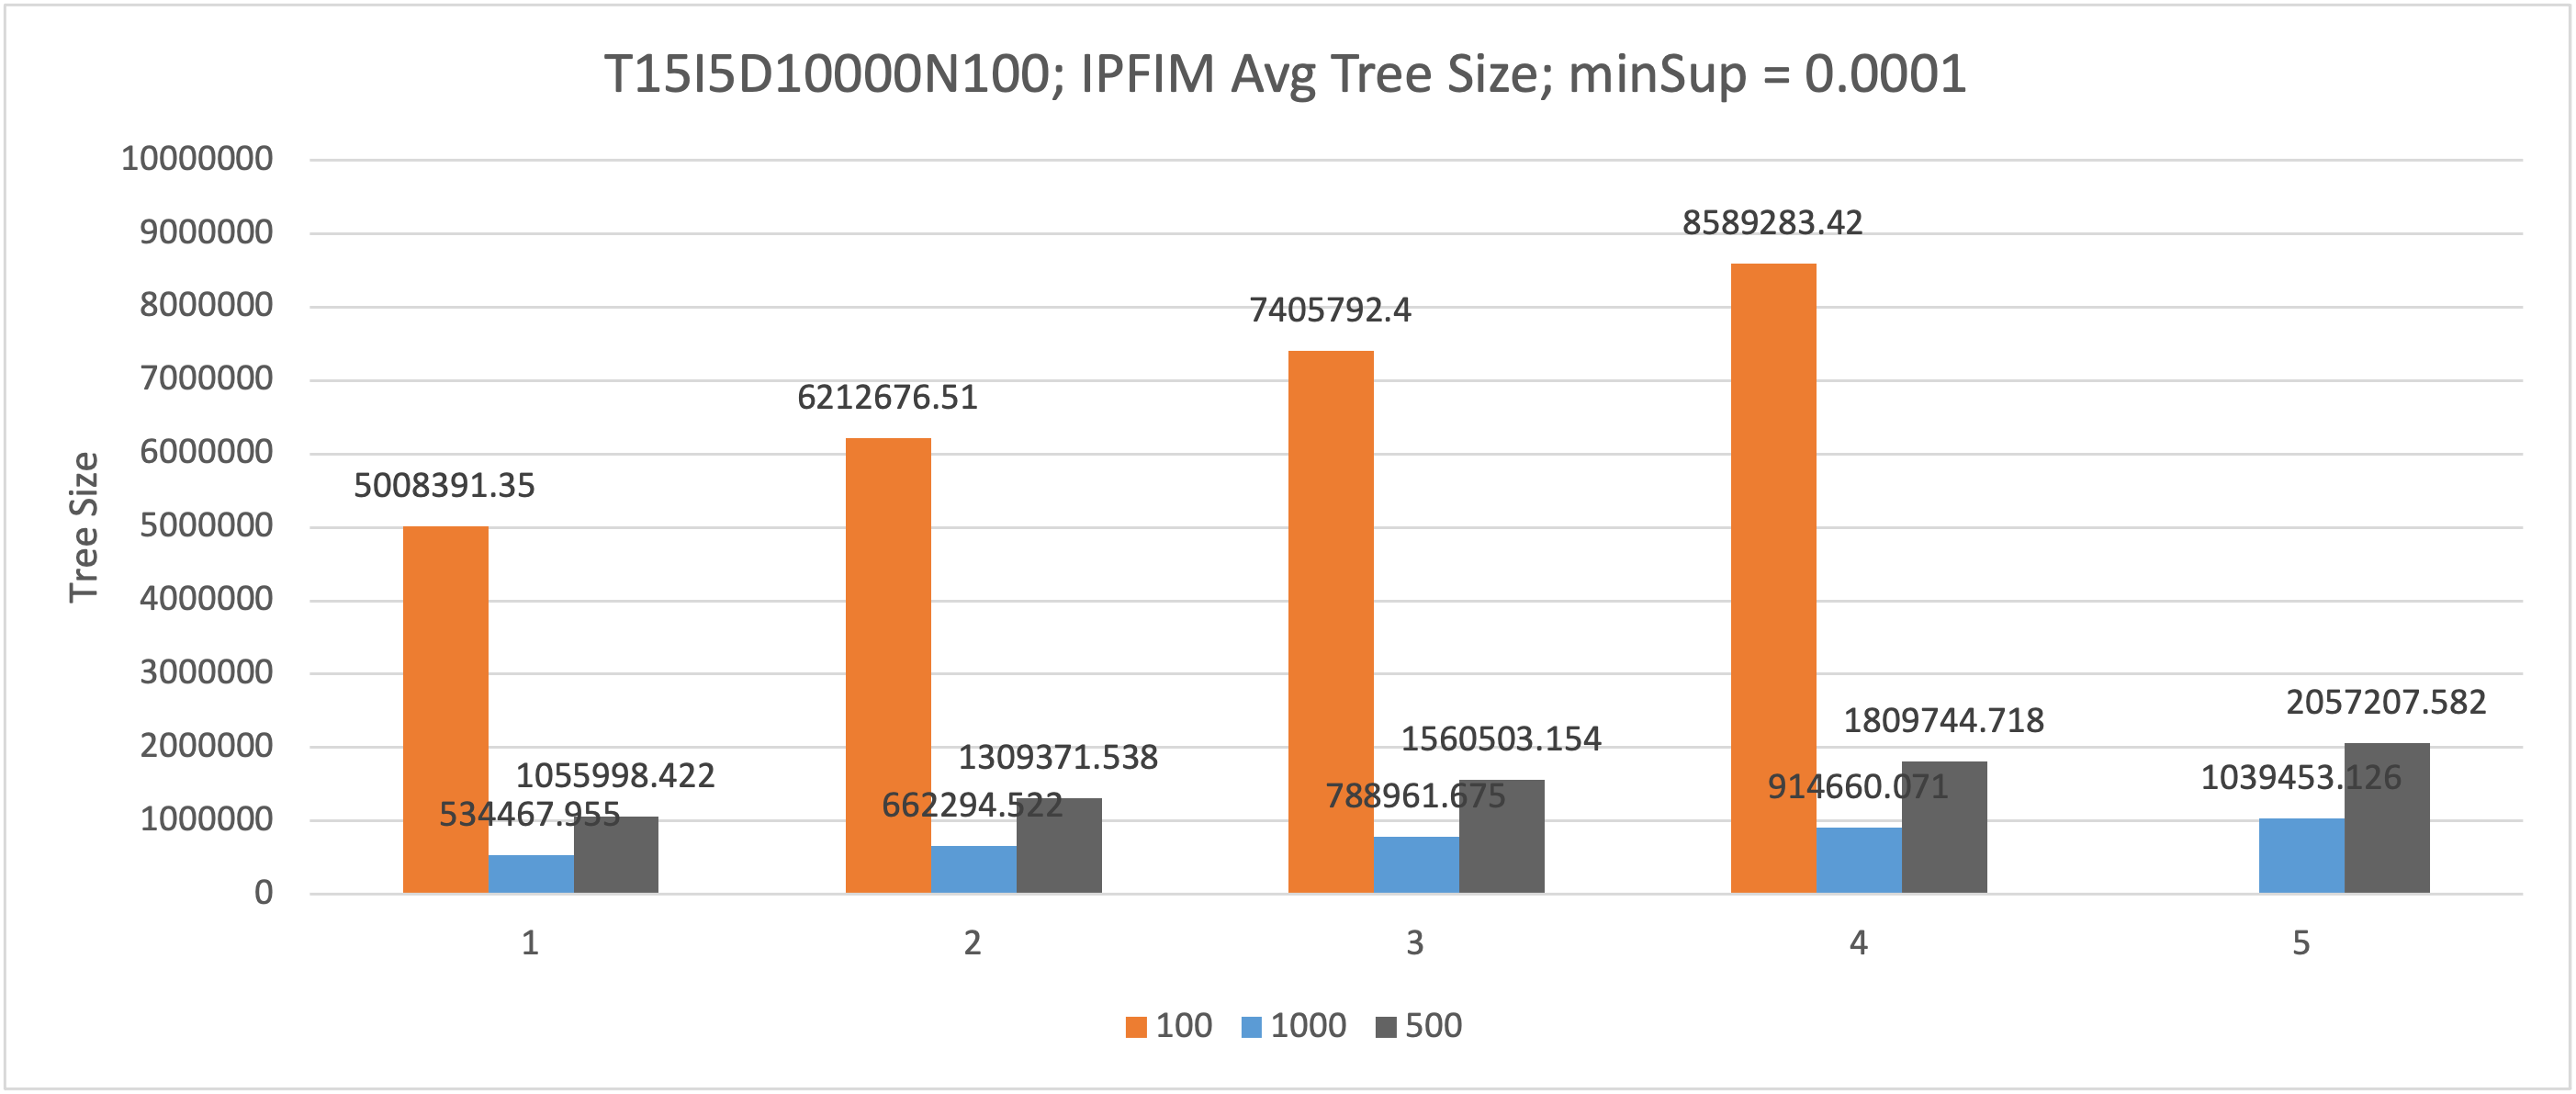
\includegraphics[width=\linewidth ,height=\textheight, keepaspectratio]{figures/4iterations/T15I5D10000N100_AvgTree_IPFIM_0001}
  \caption{T15I5D10000N100 IPFIM Average tree size}
  \label{fig:T15I5D10000N100_AvgTree_IPFIM_0001}
\end{subfigure}
\caption{T15I5D10000N100 IPFIM Average and Max tree size for 100\textbar 1000\textbar 500 partitions}
\end{figure}


\paragraph{IPFIM-Improved}
For ~\autoref{fig:T15I5D10000N100_MaxTree_IPFIMImproved_0001} the ratio is 0.277 and 0.16 between the different partitions, however for ~\autoref{fig:T15I5D10000N100_AvgTree_IPFIMImproved_0001} it is the partitions ration - 0.2 and 0.1 (same as partitions ratio).

\begin{figure}
  \centering
  \begin{subfigure}{\linewidth}
  \centering
  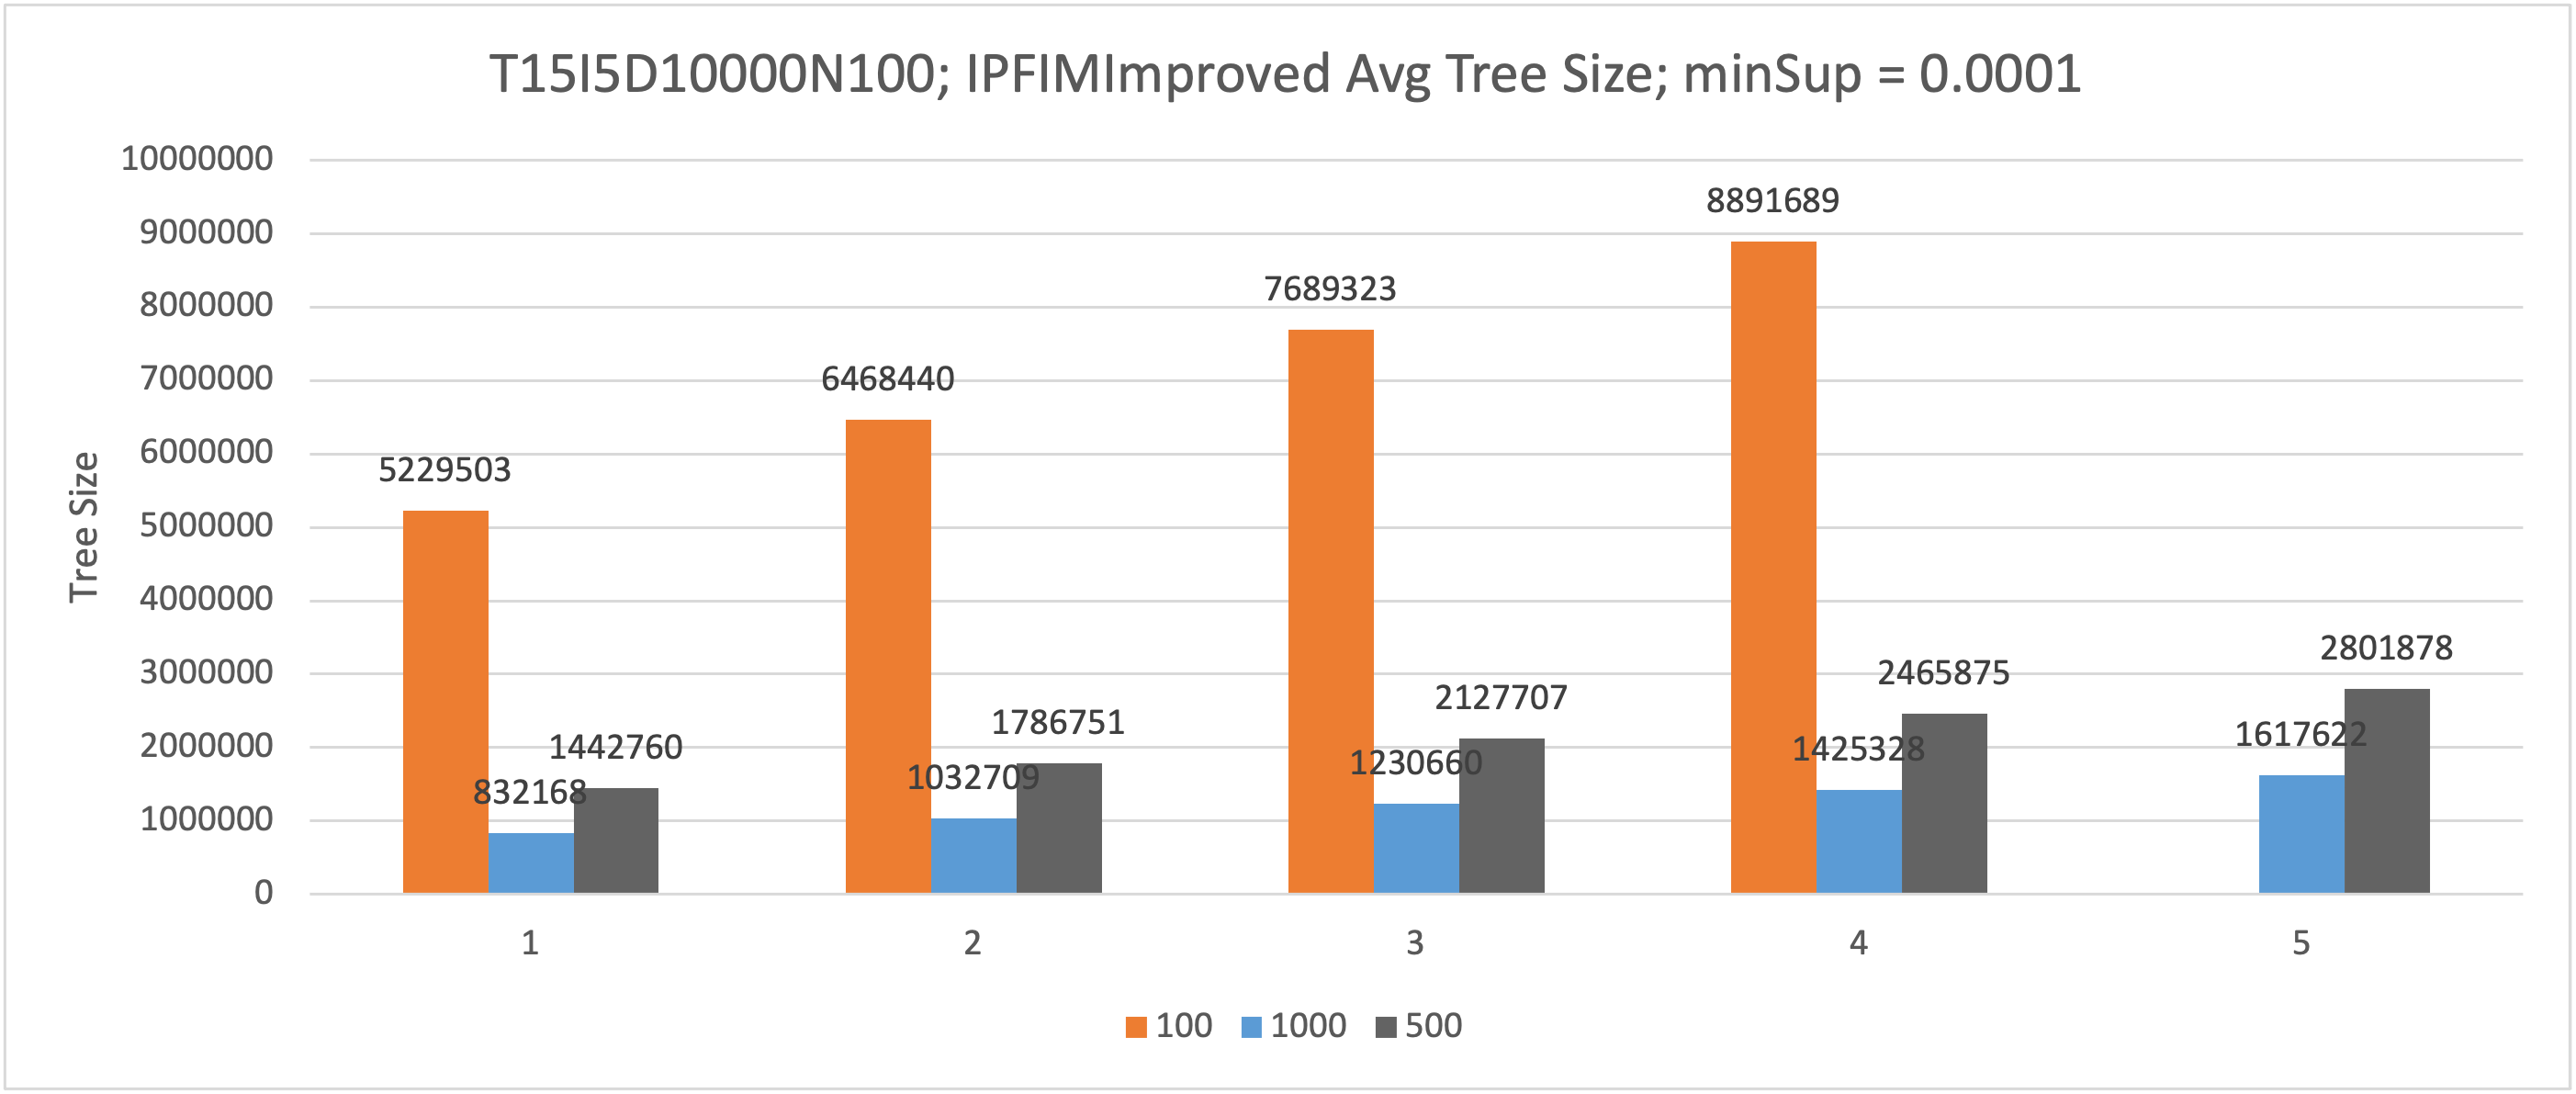
\includegraphics[width=\linewidth ,height=\textheight, keepaspectratio]{figures/4iterations/T15I5D10000N100_MaxTree_IPFIMImproved_0001}
  \caption{T15I5D10000N100 IPFIM-Improved Max tree size}
  \label{fig:T15I5D10000N100_MaxTree_IPFIMImproved_0001}
\end{subfigure}
  \begin{subfigure}{\linewidth}
  \centering
  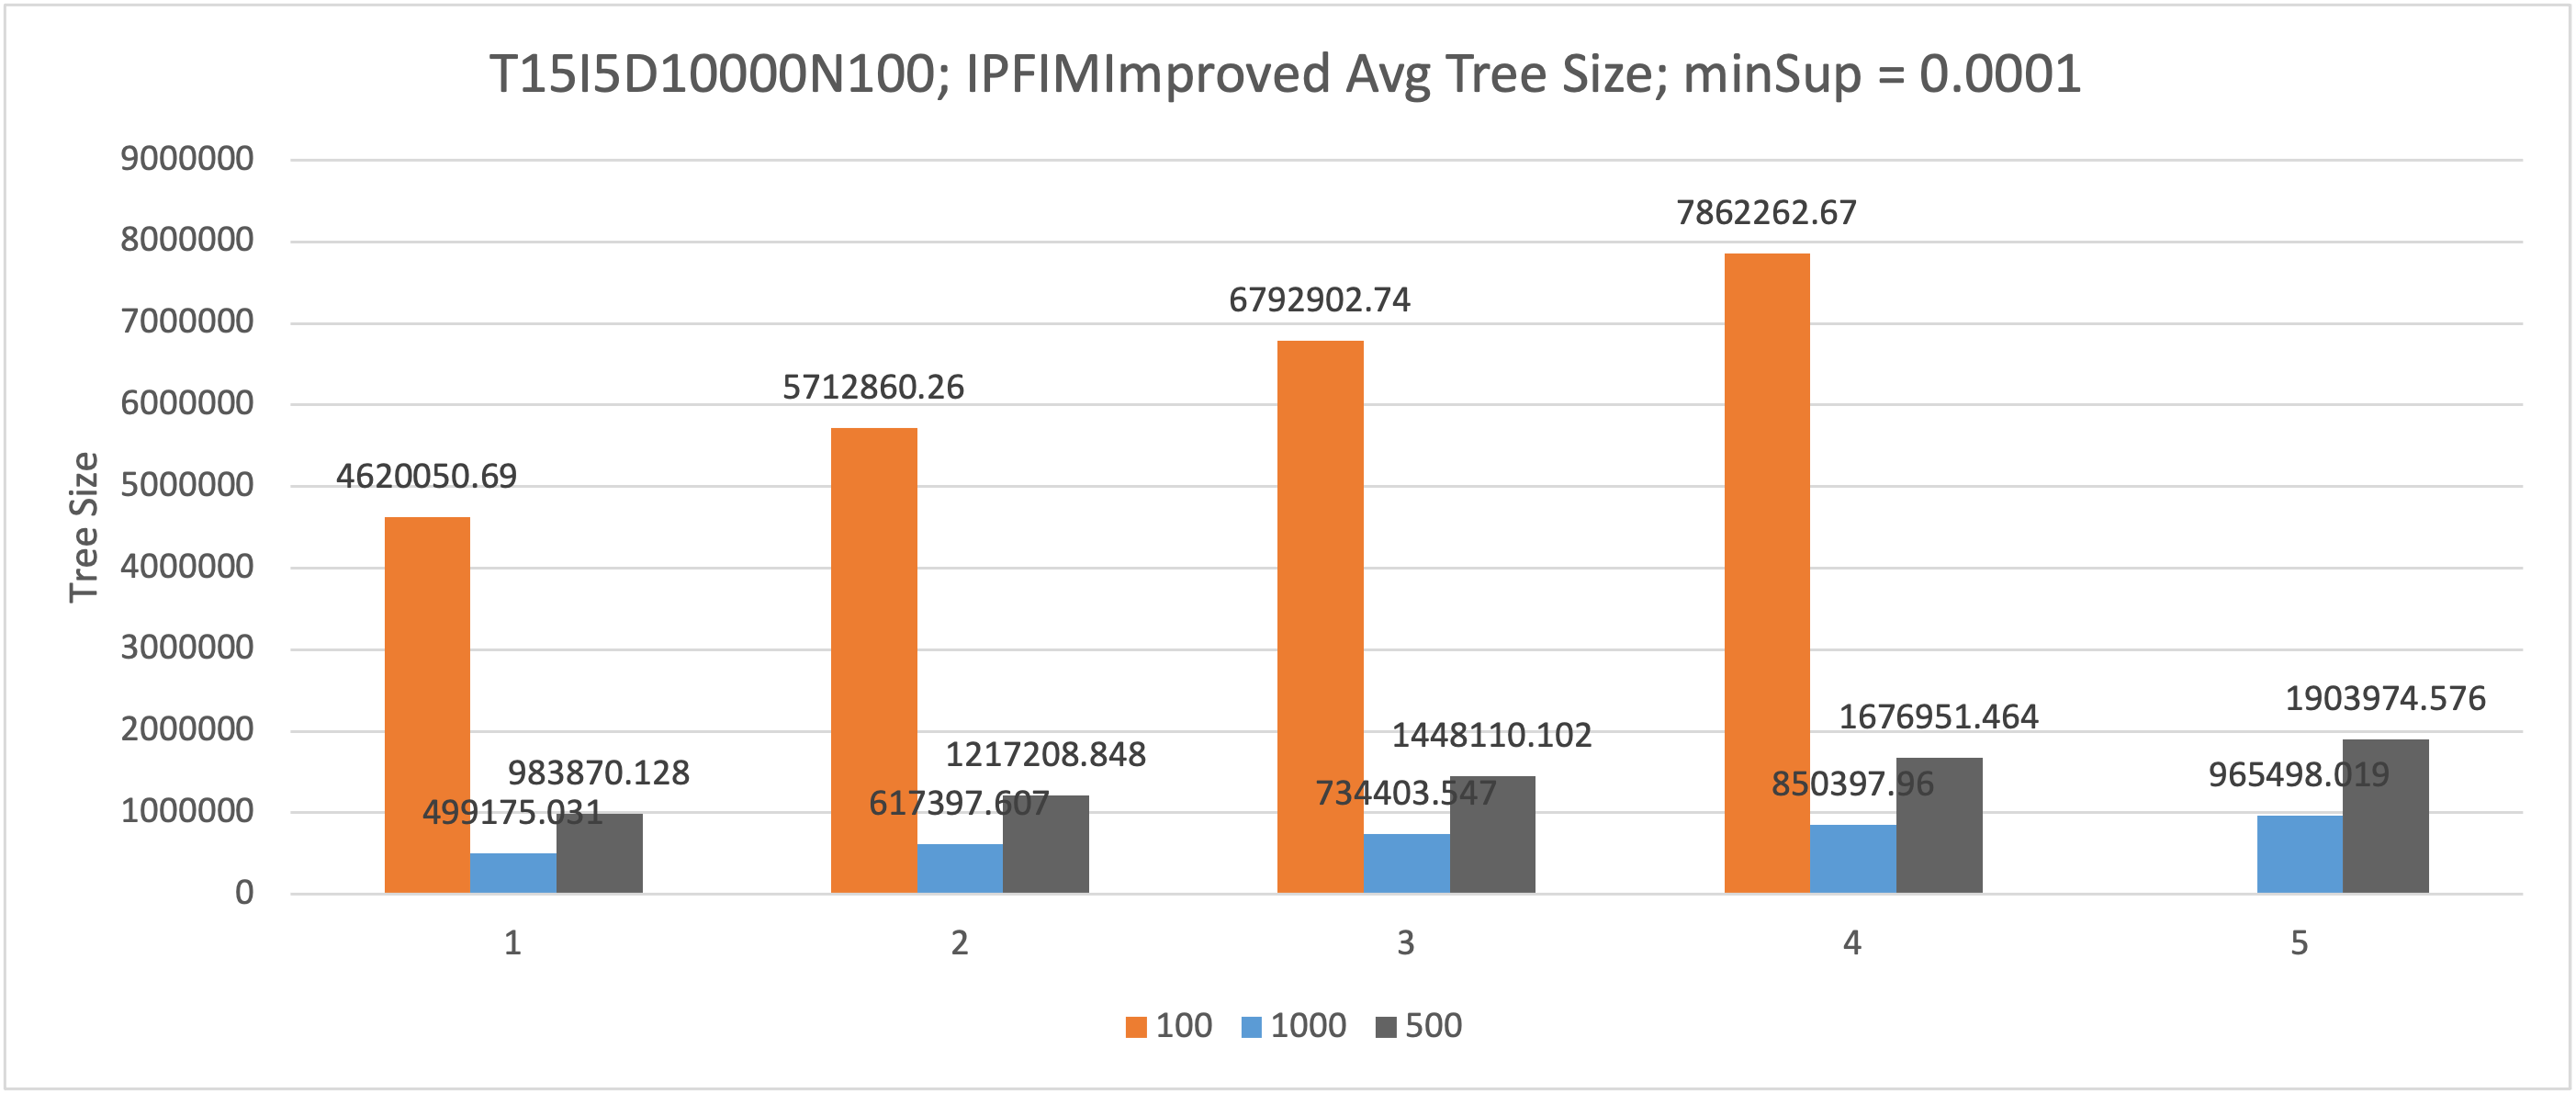
\includegraphics[width=\linewidth ,height=\textheight, keepaspectratio]{figures/4iterations/T15I5D10000N100_AvgTree_IPFIMImproved_0001}
  \caption{T15I5D10000N100 IPFIM-Improved Average tree size}
  \label{fig:T15I5D10000N100_AvgTree_IPFIMImproved_0001}
\end{subfigure}
\caption{T15I5D10000N100 IPFIM-Improved Average and Max tree size for 100\textbar 1000\textbar 500 partitions,  minSup = 0.0001, minMinSup = 0.1}
\end{figure}

\paragraph{Set-Cover IPFIM}
For ~\autoref{fig:T15I5D10000N100_MaxTree_SetCover_0001} the ratio is 0.27 and 0.16 between the different partitions, after the repartition, the max size are the same as the algorithm sets the same partition size. However for ~\autoref{fig:T15I5D10000N100_AvgTree_SetCover_0001} although partitions ration - 0.2 and 0.1 (same as partitions ratio), the average size of the partitions is much more balanced,. The reason for not having same sizes, is that some partitions remained as is, and where not affected by the recalculation. 

\begin{figure}
  \centering
  \begin{subfigure}{\linewidth}
  \centering
  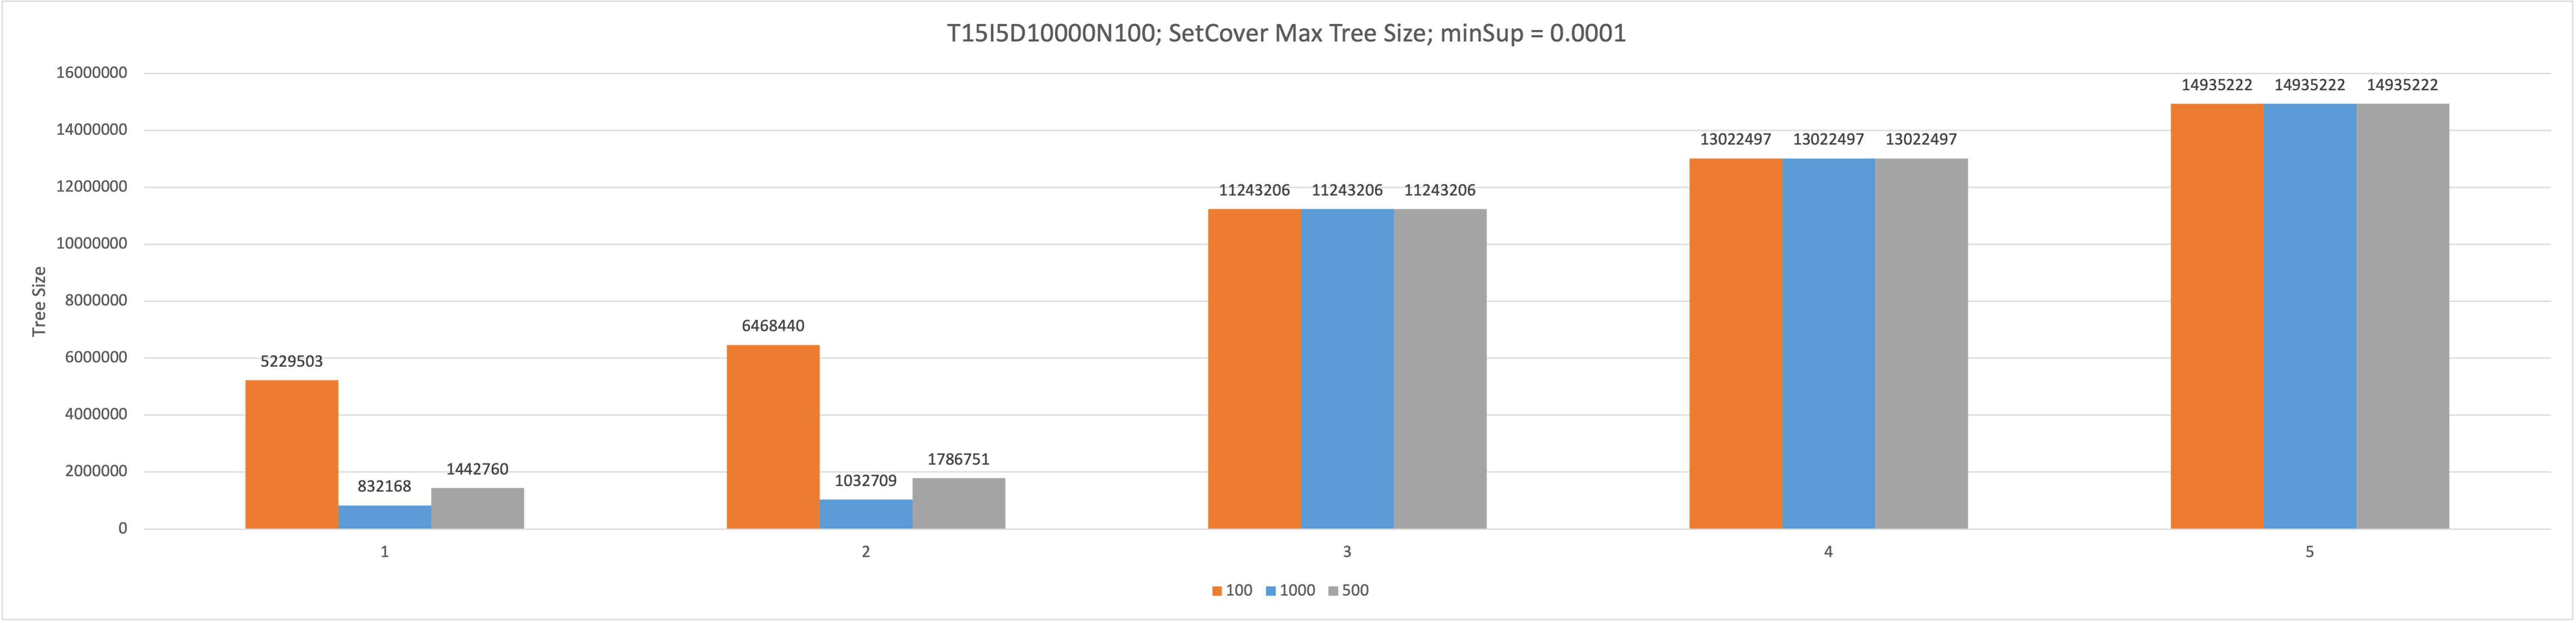
\includegraphics[width=\linewidth ,height=\textheight, keepaspectratio]{figures/4iterations/T15I5D10000N100_MaxTree_SetCover_0001}
  \caption{T15I5D10000N100 Set Cover IPFIM Max tree size}
  \label{fig:T15I5D10000N100_MaxTree_SetCover_0001}
\end{subfigure}
  \begin{subfigure}{\linewidth}
  \centering
  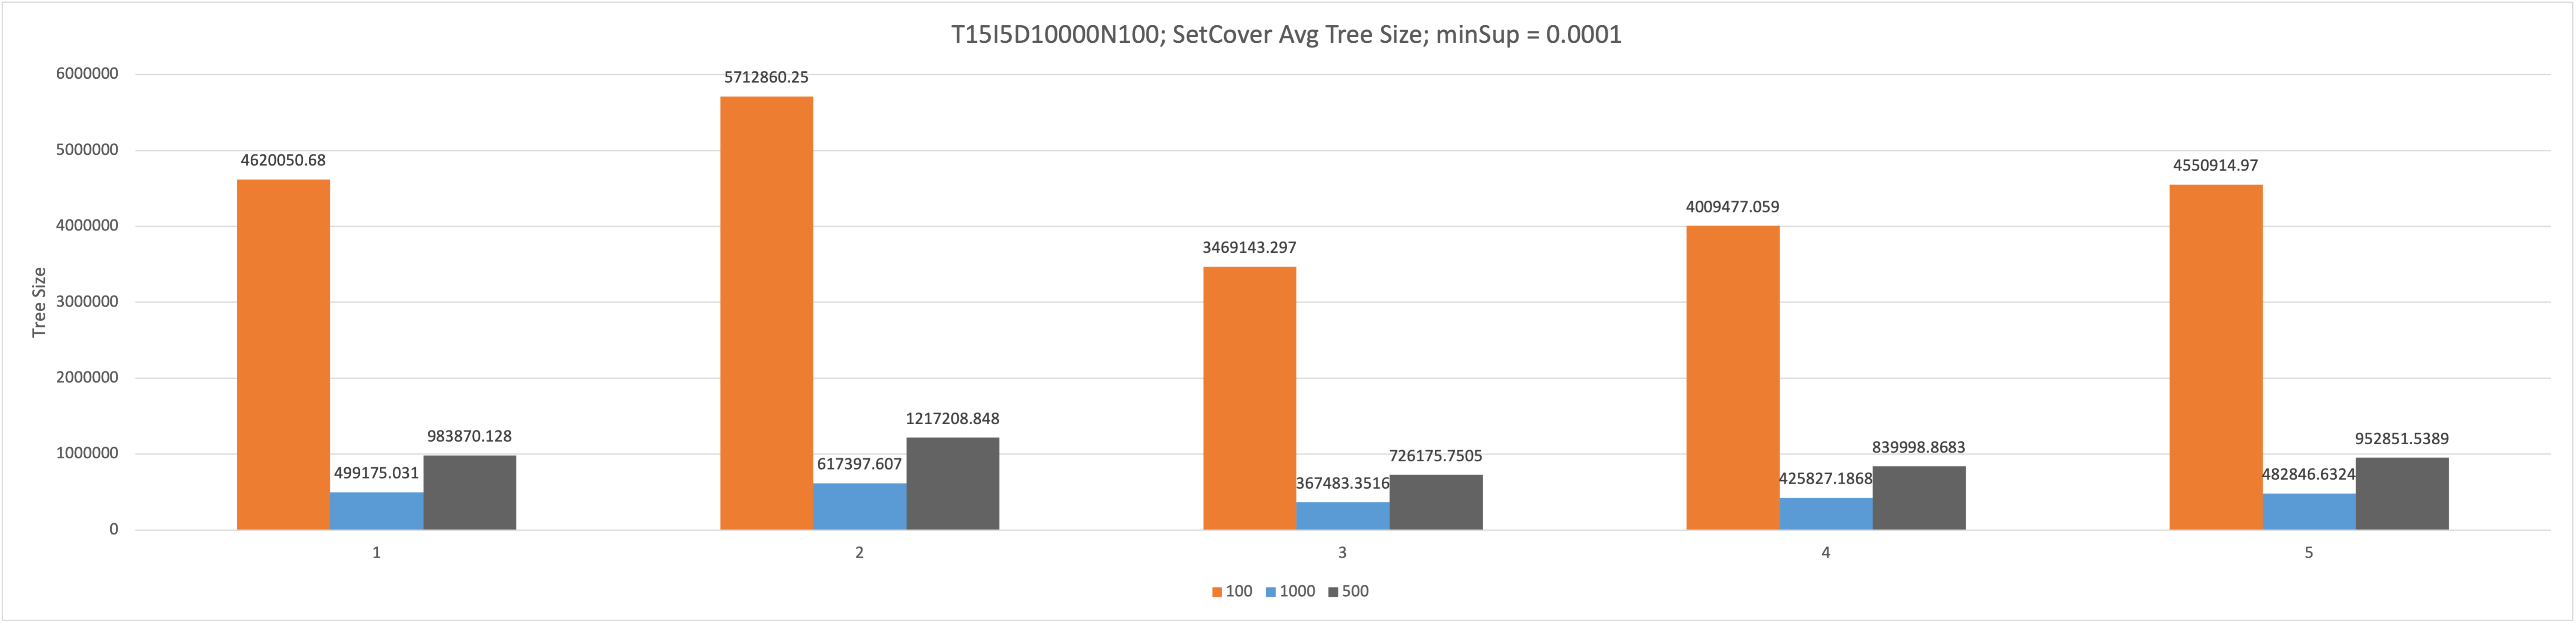
\includegraphics[width=\linewidth ,height=\textheight, keepaspectratio]{figures/4iterations/T15I5D10000N100_AvgTree_SetCover_0001}
  \caption{T15I5D10000N100 Set Cover IPFIM Average tree size}
  \label{fig:T15I5D10000N100_AvgTree_SetCover_0001}
\end{subfigure}
\caption{T15I5D10000N100 Set Cover IPFIM Average and Max tree size for 100\textbar 1000\textbar 500 partitions}
\end{figure}

\subsection{Tree size evaluation - Comparison}
~\autoref{fig:T15I5D10000N100_AvgTree_Partitins1000_0001} and ~\autoref{fig:kosarak_AvgTree_Partitins1000_001} present the comparison of average tree size for ~\autoref{data:10Msynt} and ~\autoref{data:kosarak}. 



\begin{figure}
  \centering
  \begin{subfigure}{\linewidth}
  \centering
  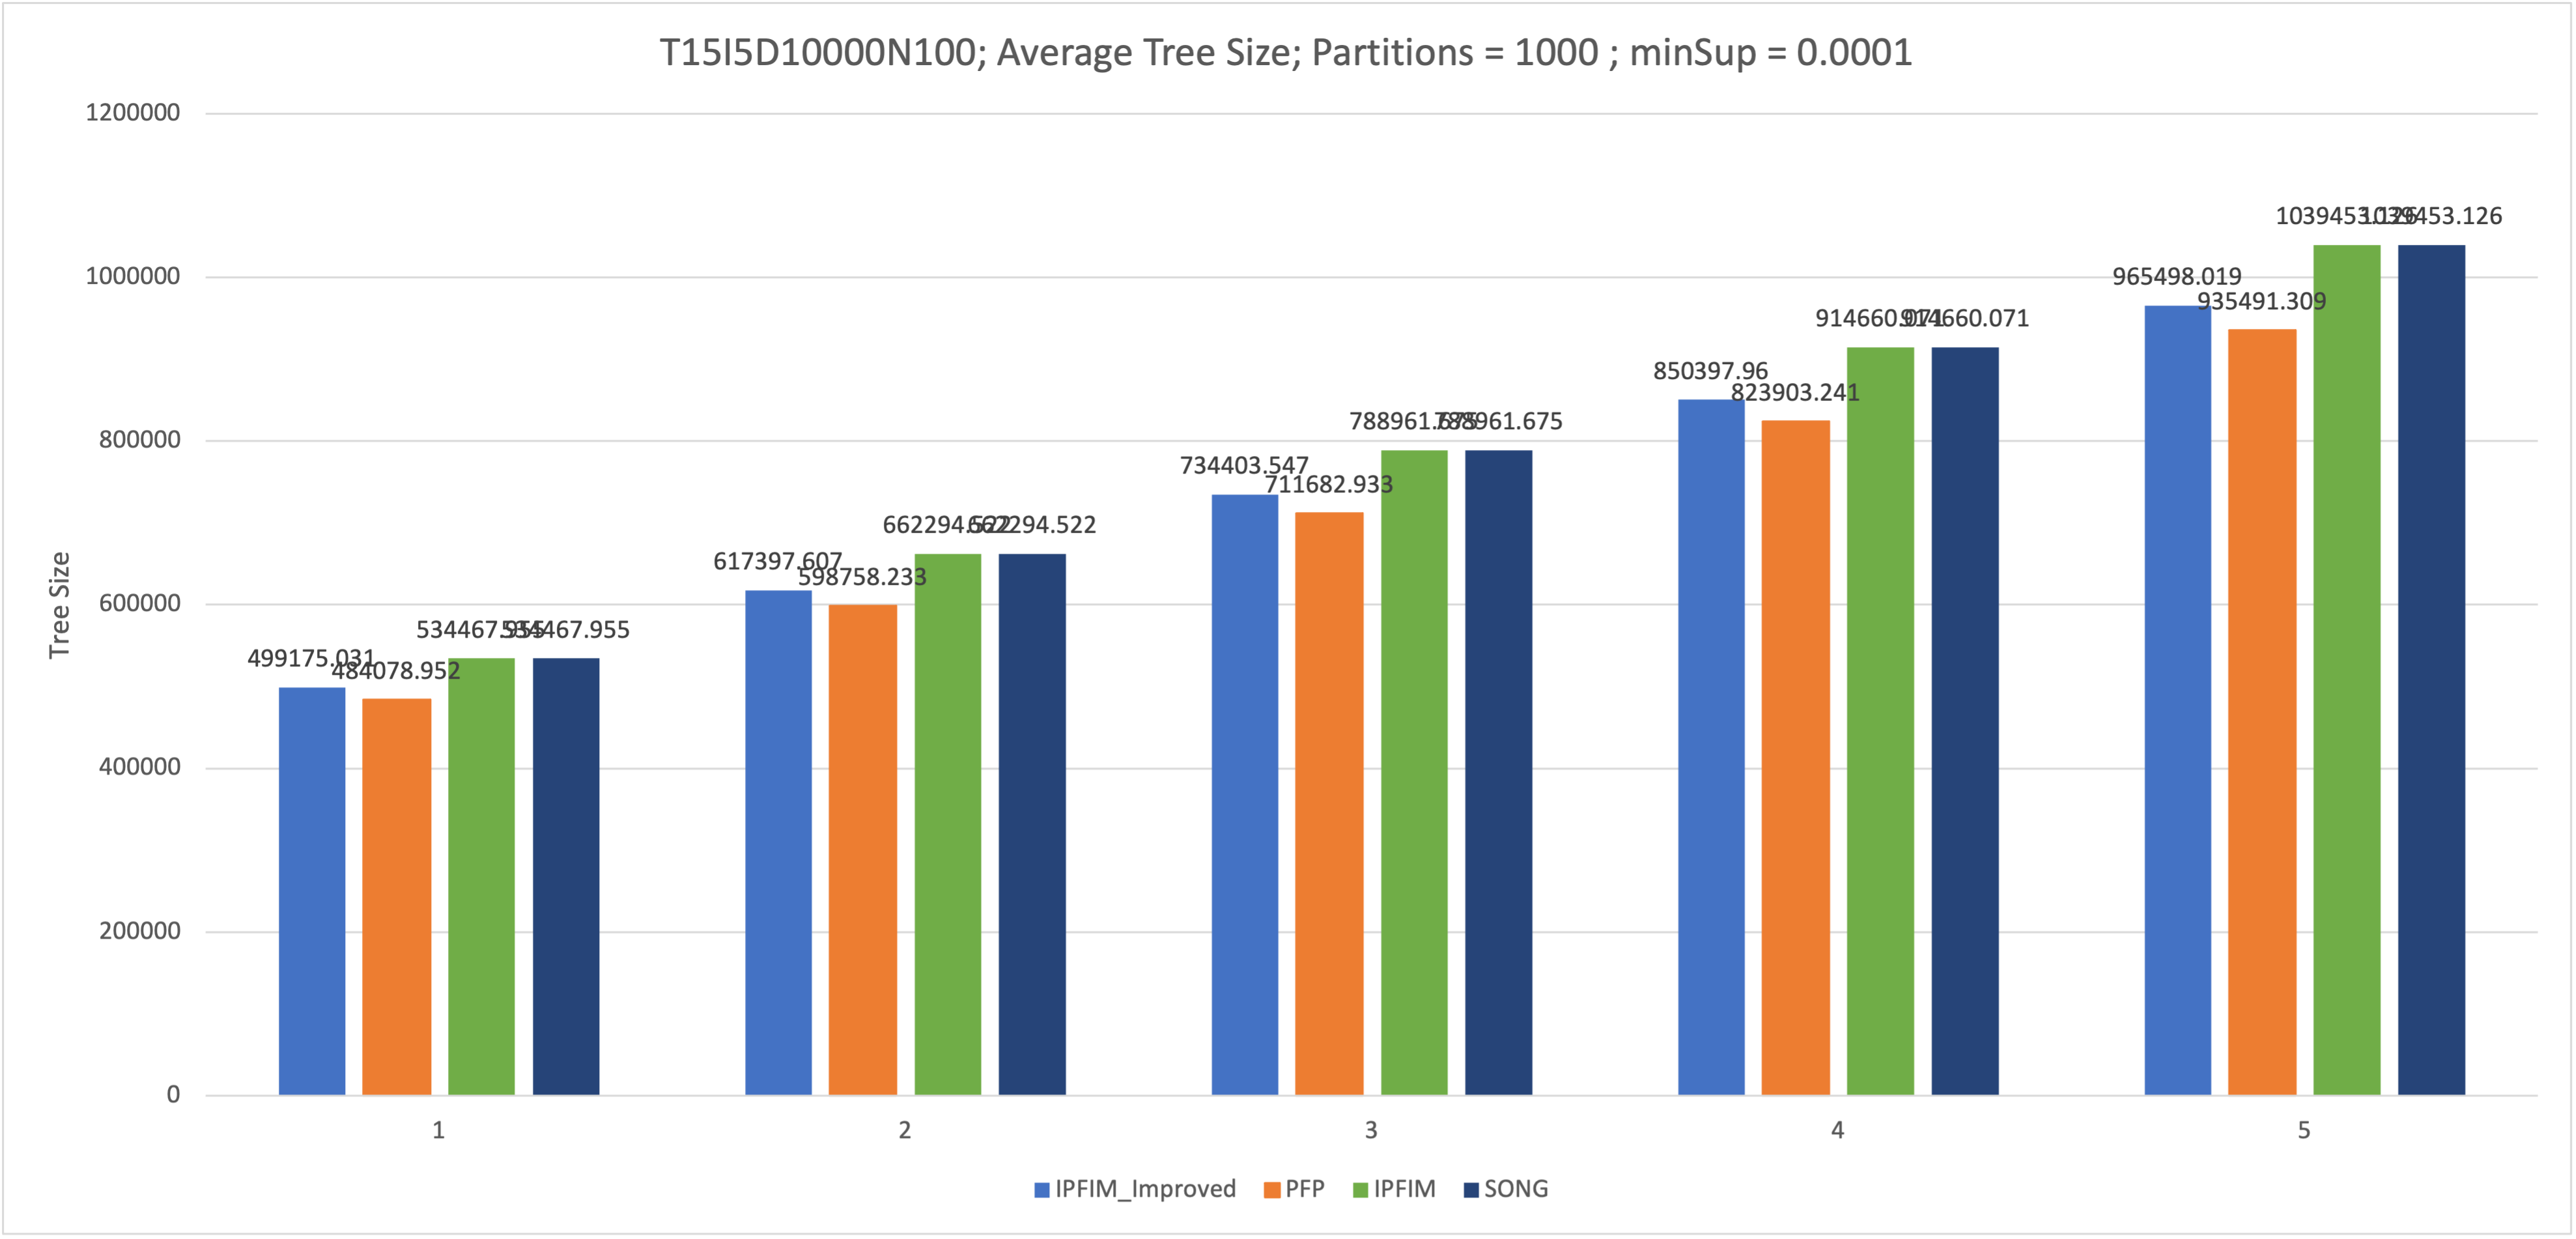
\includegraphics[width=\linewidth ,height=\textheight, keepaspectratio]{figures/4iterations/T15I5D10000N100_AvgTree_Partitins1000_0001}
  \caption{T15I5D10000N100 tree size comparison}
  \label{fig:T15I5D10000N100_AvgTree_Partitins1000_0001}
\end{subfigure}
  \begin{subfigure}{\linewidth}
  \centering
  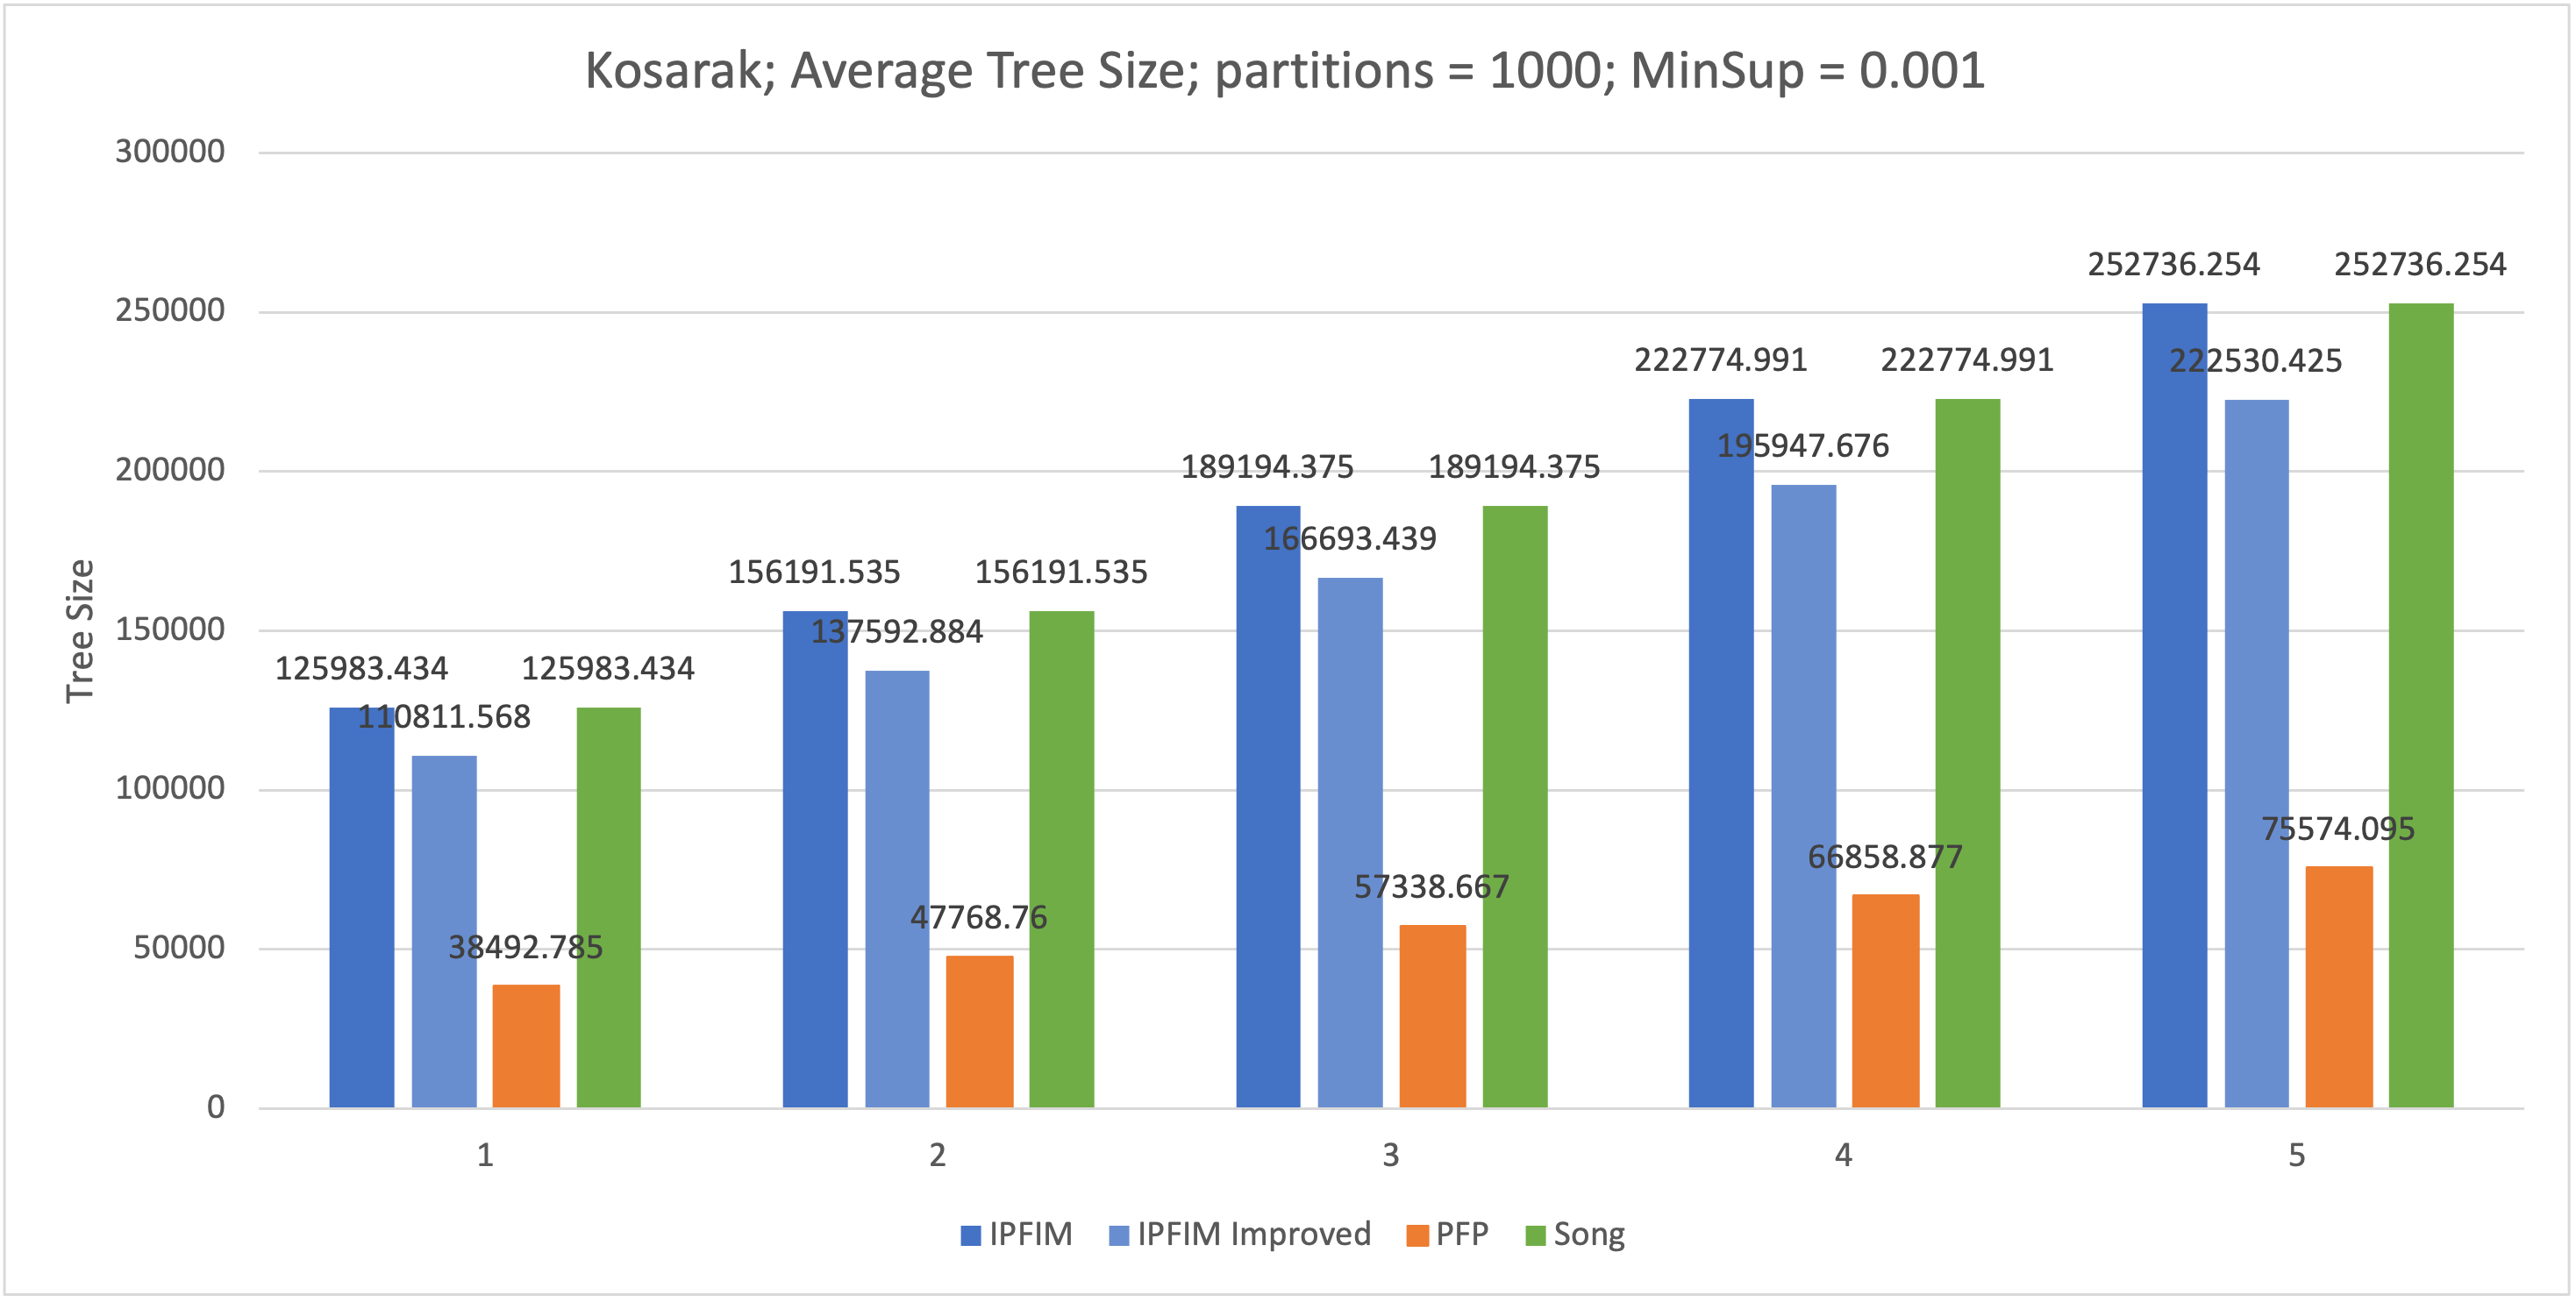
\includegraphics[width=\linewidth ,height=\textheight, keepaspectratio]{figures/4iterations/kosarak_AvgTree_Partitins1000_001}
  \caption{Kosarak tree size comparison}
  \label{fig:kosarak_AvgTree_Partitins1000_001}
\end{subfigure}
\caption{Tree size comparison for 1000 partitions}
\end{figure}

